%%%%%%%%%%%%%%%%%%%%%%%%%%%%%%%%%%%%%%%%%%%%%%%%%%%%%%%%%%%%%%%
%% BRIEF VERSION OF OXFORD THESIS TEMPLATE FOR CHAPTER PREVIEWS

%%%%% CHOOSE PAGE LAYOUT
% format for PDF output (ie equal margins, no extra blank pages):
\documentclass[a4paper,nobind]{templates/ociamthesis}

% UL 5 January 2021 - add packages used by kableExtra
\usepackage{booktabs}
\usepackage{longtable}
\usepackage{array}
\usepackage{multirow}
\usepackage{wrapfig}
\usepackage{colortbl}
\usepackage{pdflscape}
\usepackage{tabu}
\usepackage{threeparttable}
\usepackage{threeparttablex}
\usepackage[normalem]{ulem}
\usepackage{makecell}
\usepackage[colorlinks=false,pdfpagelabels,hidelinks=]{hyperref}
\usepackage{float}


%UL set section header spacing
\usepackage{titlesec}
% 
\titlespacing\subsubsection{0pt}{24pt plus 4pt minus 2pt}{0pt plus 2pt minus 2pt}

% UL 30 Nov 2018 pandoc puts lists in 'tightlist' command when no space between bullet points in Rmd file
\providecommand{\tightlist}{%
  \setlength{\itemsep}{0pt}\setlength{\parskip}{0pt}}
 
% UL 1 Dec 2018, fix to include code in shaded environments
\usepackage{color}
\usepackage{fancyvrb}
\newcommand{\VerbBar}{|}
\newcommand{\VERB}{\Verb[commandchars=\\\{\}]}
\DefineVerbatimEnvironment{Highlighting}{Verbatim}{commandchars=\\\{\}}
% Add ',fontsize=\small' for more characters per line
\usepackage{framed}
\definecolor{shadecolor}{RGB}{248,248,248}
\newenvironment{Shaded}{\begin{snugshade}}{\end{snugshade}}
\newcommand{\AlertTok}[1]{\textcolor[rgb]{0.94,0.16,0.16}{#1}}
\newcommand{\AnnotationTok}[1]{\textcolor[rgb]{0.56,0.35,0.01}{\textbf{\textit{#1}}}}
\newcommand{\AttributeTok}[1]{\textcolor[rgb]{0.77,0.63,0.00}{#1}}
\newcommand{\BaseNTok}[1]{\textcolor[rgb]{0.00,0.00,0.81}{#1}}
\newcommand{\BuiltInTok}[1]{#1}
\newcommand{\CharTok}[1]{\textcolor[rgb]{0.31,0.60,0.02}{#1}}
\newcommand{\CommentTok}[1]{\textcolor[rgb]{0.56,0.35,0.01}{\textit{#1}}}
\newcommand{\CommentVarTok}[1]{\textcolor[rgb]{0.56,0.35,0.01}{\textbf{\textit{#1}}}}
\newcommand{\ConstantTok}[1]{\textcolor[rgb]{0.00,0.00,0.00}{#1}}
\newcommand{\ControlFlowTok}[1]{\textcolor[rgb]{0.13,0.29,0.53}{\textbf{#1}}}
\newcommand{\DataTypeTok}[1]{\textcolor[rgb]{0.13,0.29,0.53}{#1}}
\newcommand{\DecValTok}[1]{\textcolor[rgb]{0.00,0.00,0.81}{#1}}
\newcommand{\DocumentationTok}[1]{\textcolor[rgb]{0.56,0.35,0.01}{\textbf{\textit{#1}}}}
\newcommand{\ErrorTok}[1]{\textcolor[rgb]{0.64,0.00,0.00}{\textbf{#1}}}
\newcommand{\ExtensionTok}[1]{#1}
\newcommand{\FloatTok}[1]{\textcolor[rgb]{0.00,0.00,0.81}{#1}}
\newcommand{\FunctionTok}[1]{\textcolor[rgb]{0.00,0.00,0.00}{#1}}
\newcommand{\ImportTok}[1]{#1}
\newcommand{\InformationTok}[1]{\textcolor[rgb]{0.56,0.35,0.01}{\textbf{\textit{#1}}}}
\newcommand{\KeywordTok}[1]{\textcolor[rgb]{0.13,0.29,0.53}{\textbf{#1}}}
\newcommand{\NormalTok}[1]{#1}
\newcommand{\OperatorTok}[1]{\textcolor[rgb]{0.81,0.36,0.00}{\textbf{#1}}}
\newcommand{\OtherTok}[1]{\textcolor[rgb]{0.56,0.35,0.01}{#1}}
\newcommand{\PreprocessorTok}[1]{\textcolor[rgb]{0.56,0.35,0.01}{\textit{#1}}}
\newcommand{\RegionMarkerTok}[1]{#1}
\newcommand{\SpecialCharTok}[1]{\textcolor[rgb]{0.00,0.00,0.00}{#1}}
\newcommand{\SpecialStringTok}[1]{\textcolor[rgb]{0.31,0.60,0.02}{#1}}
\newcommand{\StringTok}[1]{\textcolor[rgb]{0.31,0.60,0.02}{#1}}
\newcommand{\VariableTok}[1]{\textcolor[rgb]{0.00,0.00,0.00}{#1}}
\newcommand{\VerbatimStringTok}[1]{\textcolor[rgb]{0.31,0.60,0.02}{#1}}
\newcommand{\WarningTok}[1]{\textcolor[rgb]{0.56,0.35,0.01}{\textbf{\textit{#1}}}}

%UL 2 Dec 2018 add a bit of white space before and after code blocks
\renewenvironment{Shaded}
{
  \vspace{10pt}%
  \begin{snugshade}%
}{%
  \end{snugshade}%
  \vspace{8pt}%
}
%UL 2 Dec 2018 reduce whitespace around verbatim environments
\usepackage{etoolbox}
\makeatletter
\preto{\@verbatim}{\topsep=0pt \partopsep=0pt }
\makeatother

%UL 28 Mar 2019, enable strikethrough
\usepackage[normalem]{ulem}

%UL use soul package for correction highlighting
\usepackage{soul}
\usepackage{xcolor}
\newcommand{\ctext}[3][RGB]{%
  \begingroup
  \definecolor{hlcolor}{#1}{#2}\sethlcolor{hlcolor}%
  \hl{#3}%
  \endgroup
}
\soulregister\ref7
\soulregister\cite7
\soulregister\autocite7
\soulregister\textcite7
\soulregister\pageref7

%UL 3 Nov 2019, avoid mysterious error from not having hyperref included
\usepackage{hyperref}

%%%%% SELECT YOUR DRAFT OPTIONS
% Three options going on here; use in any combination.  But remember to turn the first two off before
% generating a PDF to send to the printer!

% This adds a "DRAFT" footer to every normal page.  (The first page of each chapter is not a "normal" page.)

% This highlights (in blue) corrections marked with (for words) \mccorrect{blah} or (for whole
% paragraphs) \begin{mccorrection} . . . \end{mccorrection}.  This can be useful for sending a PDF of
% your corrected thesis to your examiners for review.  Turn it off, and the blue disappears.

%%%%% BIBLIOGRAPHY SETUP
% Note that your bibliography will require some tweaking depending on your department, preferred format, etc.
% The options included below are just very basic "sciencey" and "humanitiesey" options to get started.
% If you've not used LaTeX before, I recommend reading a little about biblatex/biber and getting started with it.
% If you're already a LaTeX pro and are used to natbib or something, modify as necessary.
% Either way, you'll have to choose and configure an appropriate bibliography format...

% The science-type option: numerical in-text citation with references in order of appearance.
% \usepackage[style=numeric-comp, sorting=none, backend=biber, doi=false, isbn=false]{biblatex}
% \newcommand*{\bibtitle}{References}

% The humanities-type option: author-year in-text citation with an alphabetical works cited.
% \usepackage[style=authoryear, sorting=nyt, backend=biber, maxcitenames=2, useprefix, doi=false, isbn=false]{biblatex}
% \newcommand*{\bibtitle}{Works Cited}

%UL 3 Dec 2018: set this from YAML in index.Rmd
\usepackage[style=numeric-comp, sorting=none, backend=biber, doi=false, isbn=false]{biblatex}
\newcommand*{\bibtitle}{References}

% This makes the bibliography left-aligned (not 'justified') and slightly smaller font.
\renewcommand*{\bibfont}{\raggedright\small}

% Change this to the name of your .bib file (usually exported from a citation manager like Zotero or EndNote).
\addbibresource{references.bib}

%%%%% YOUR OWN PERSONAL MACROS
% This is a good place to dump your own LaTeX macros as they come up.

% To make text superscripts shortcuts
	\renewcommand{\th}{\textsuperscript{th}} % ex: I won 4\th place
	\newcommand{\nd}{\textsuperscript{nd}}
	\renewcommand{\st}{\textsuperscript{st}}
	\newcommand{\rd}{\textsuperscript{rd}}

%%%%% THE ACTUAL DOCUMENT STARTS HERE
\begin{document}

%%%%% CHOOSE YOUR LINE SPACING HERE
% This is the official option.  Use it for your submission copy and library copy:
\setlength{\textbaselineskip}{22pt plus2pt}
% This is closer spacing (about 1.5-spaced) that you might prefer for your personal copies:
%\setlength{\textbaselineskip}{18pt plus2pt minus1pt}

% UL: You can set the general paragraph spacing here - I've set it to 2pt (was 0) so
% it's less claustrophobic
\setlength{\parskip}{2pt plus 1pt}

% Leave this line alone; it gets things started for the real document.
\setlength{\baselineskip}{\textbaselineskip}

% all your chapters and appendices will appear here
\hypertarget{Introduction}{%
\chapter{Sources of Finance for Microfinance Institutions in Africa}\label{Introduction}}

\minitoc 
\chaptermark{Financing MFIs in Africa}

\textbf{ABSTRACT}

\begin{quote}
We examine four sources of finance, and their associated financial structure for microfinance institutions (MFIs) in Africa: debt-equity ratio (leverage) and capital to assets ratio (equity), deposits to assets ratio (deposits), and donations to assets ratio (donations). Our analysis shows that at the firm level, size, age, legal status, and profitability drive financing alternatives in line with theory. For example, asset structure varies inversely with leverage. At the country-level, institutional quality (KKM) varies inversely with deposits and donations. Intersstingly, coefficients of financial development and education variables are not significant across all financial structure proxies, going against stylised facts on the macro-level drivers of firms' financing structure. We find that firm-llevel that firm-level factors are more relevant in determining the financing structure of MFIs.
\end{quote}

\newpage

\begin{Shaded}
\begin{Highlighting}[]
\DocumentationTok{\#\# legal traditions }
\DocumentationTok{\#\#\# Common law countries in Africa}
\NormalTok{common }\OtherTok{\textless{}{-}} \FunctionTok{tibble}\NormalTok{(}\AttributeTok{country =} \FunctionTok{c}\NormalTok{(}\StringTok{"Botswana"}\NormalTok{, }\StringTok{"Gambia, The"}\NormalTok{, }\StringTok{"Ghana"}\NormalTok{, }\StringTok{"Kenya"}\NormalTok{, }\StringTok{"Lesotho"}\NormalTok{, }\StringTok{"Liberia"}\NormalTok{, }\StringTok{"Malawi"}\NormalTok{, }\StringTok{"Namibia"}\NormalTok{, }\StringTok{"Nigeria"}\NormalTok{, }\StringTok{"Sierra Leone"}\NormalTok{, }\StringTok{"South Africa"}\NormalTok{, }\StringTok{"South Sudan"}\NormalTok{, }\StringTok{"Sudan"}\NormalTok{, }\StringTok{"Eswatini"}\NormalTok{, }\StringTok{"Tanzania"}\NormalTok{, }\StringTok{"Uganda"}\NormalTok{, }\StringTok{"Zambia"}\NormalTok{, }\StringTok{"Zimbabwe"}\NormalTok{), }\AttributeTok{trad =} \FunctionTok{c}\NormalTok{(}\FunctionTok{rep}\NormalTok{(}\StringTok{"common"}\NormalTok{, }\DecValTok{18}\NormalTok{)))}

\DocumentationTok{\#\#\# Civil law countries in Africa}
\NormalTok{civil }\OtherTok{\textless{}{-}} \FunctionTok{tibble}\NormalTok{(}\AttributeTok{country =} \FunctionTok{c}\NormalTok{(}\StringTok{"Algeria"}\NormalTok{, }\StringTok{"Benin"}\NormalTok{, }\StringTok{"Burkina Faso"}\NormalTok{, }\StringTok{"Cameroon"}\NormalTok{, }\StringTok{"Central African Republic"}\NormalTok{, }\StringTok{"Chad"}\NormalTok{, }\StringTok{"Comoros"}\NormalTok{, }\StringTok{"Congo, Rep."}\NormalTok{, }\StringTok{"Cote d\textquotesingle{}Ivoire"}\NormalTok{, }\StringTok{"Gabon"}\NormalTok{, }\StringTok{"Guinea"}\NormalTok{, }\StringTok{"Madagascar"}\NormalTok{, }\StringTok{"Mali"}\NormalTok{, }\StringTok{"Mauritania"}\NormalTok{, }\StringTok{"Morocco"}\NormalTok{, }\StringTok{"Niger"}\NormalTok{, }\StringTok{"Senegal"}\NormalTok{, }\StringTok{"Togo"}\NormalTok{, }\StringTok{"Tunisia"}\NormalTok{), }\AttributeTok{trad =} \FunctionTok{c}\NormalTok{(}\FunctionTok{rep}\NormalTok{(}\StringTok{"civil"}\NormalTok{, }\DecValTok{19}\NormalTok{)))}

\DocumentationTok{\#\#\# Other legal traditions in Africa}
\NormalTok{others }\OtherTok{\textless{}{-}} \FunctionTok{tibble}\NormalTok{(}\AttributeTok{country =} \FunctionTok{c}\NormalTok{(}\StringTok{"Equatorial Guinea"}\NormalTok{, }\StringTok{"Angola"}\NormalTok{, }\StringTok{"Burundi"}\NormalTok{, }\StringTok{"Cape Verde"}\NormalTok{, }\StringTok{"Congo, Dem. Rep."}\NormalTok{, }\StringTok{"Egypt, Arab Republic of"}\NormalTok{, }\StringTok{"Ethiopia"}\NormalTok{, }\StringTok{"Eritrea"}\NormalTok{, }\StringTok{"Guinea{-}Bissau"}\NormalTok{, }\StringTok{"Mozambique"}\NormalTok{, }\StringTok{"Rwanda"}\NormalTok{), }\AttributeTok{trad =} \FunctionTok{c}\NormalTok{(}\FunctionTok{rep}\NormalTok{(}\StringTok{"others"}\NormalTok{, }\DecValTok{11}\NormalTok{)))}

\DocumentationTok{\#\#\#Putting them all together}
\NormalTok{legal }\OtherTok{\textless{}{-}} \FunctionTok{rbind}\NormalTok{(common, civil, others)}
\end{Highlighting}
\end{Shaded}

\begin{Shaded}
\begin{Highlighting}[]
\CommentTok{\# Bond market data {-} private and public bond market capitalization to GDP}
\NormalTok{bonds }\OtherTok{\textless{}{-}} \FunctionTok{read\_excel}\NormalTok{(}\StringTok{"bonds\_oluoch.xlsx"}\NormalTok{) }\SpecialCharTok{\%\textgreater{}\%} 
  
\NormalTok{  janitor}\SpecialCharTok{::}\FunctionTok{clean\_names}\NormalTok{()}
\end{Highlighting}
\end{Shaded}

\begin{Shaded}
\begin{Highlighting}[]
\CommentTok{\# Add the financial development index to the dataset}
\DocumentationTok{\#\# Countries not part of Africa}
\NormalTok{mideast }\OtherTok{\textless{}{-}} \FunctionTok{c}\NormalTok{(}\StringTok{"Bahrain"}\NormalTok{, }\StringTok{"Iran, Islamic Rep."}\NormalTok{, }\StringTok{"Iraq"}\NormalTok{, }\StringTok{"Israel"}\NormalTok{, }\StringTok{"Jordan"}\NormalTok{, }\StringTok{"Kuwait"}\NormalTok{, }\StringTok{"Lebanon"}\NormalTok{, }\StringTok{"Malta"}\NormalTok{, }\StringTok{"Oman"}\NormalTok{, }\StringTok{"Qatar"}\NormalTok{, }\StringTok{"Saudi Arabia"}\NormalTok{, }\StringTok{"Syrian Arab Republic"}\NormalTok{, }\StringTok{"United Arab Emirates"}\NormalTok{, }\StringTok{"West Bank and Gaza"}\NormalTok{, }\StringTok{"Yemen, Rep."}\NormalTok{)}

\DocumentationTok{\#\# Load the financial structure data}
\NormalTok{finstr }\OtherTok{\textless{}{-}} \FunctionTok{read\_excel}\NormalTok{(}\StringTok{"FinancialStructureDatabase20191018.xlsx"}\NormalTok{, }\AttributeTok{sheet =} \DecValTok{4}\NormalTok{) }\SpecialCharTok{\%\textgreater{}\%} 
  
  \DocumentationTok{\#\# Select desired variables}
  \FunctionTok{select}\NormalTok{(country, region, year, pcrdbgdp, stmktcap, stvaltraded, stturnover, listco\_pc) }\SpecialCharTok{\%\textgreater{}\%} 
  
  \DocumentationTok{\#\#\# Filter out regions not in Africa or middle east}
  \FunctionTok{filter}\NormalTok{(region }\SpecialCharTok{==} \StringTok{"Sub{-}Saharan Africa"} \SpecialCharTok{|}\NormalTok{ region }\SpecialCharTok{==} \StringTok{"Middle East \& North Africa"}\NormalTok{) }\SpecialCharTok{\%\textgreater{}\%} 
  \DocumentationTok{\#\#\# Filter out countries in middle east and select year 1999 onwards}
  \FunctionTok{filter}\NormalTok{(}\SpecialCharTok{!}\NormalTok{country }\SpecialCharTok{\%in\%}\NormalTok{ mideast, year }\SpecialCharTok{\textgreater{}=} \DecValTok{1999}\NormalTok{) }\SpecialCharTok{\%\textgreater{}\%} 
  
\DocumentationTok{\#\# Replace NAs}
          \FunctionTok{group\_by}\NormalTok{(country) }\SpecialCharTok{\%\textgreater{}\%} 
  
          \FunctionTok{mutate}\NormalTok{(}\AttributeTok{pcrdbgdp =} \FunctionTok{replace\_na}\NormalTok{(pcrdbgdp, }\FunctionTok{median}\NormalTok{(pcrdbgdp, }\AttributeTok{na.rm =} \ConstantTok{TRUE}\NormalTok{)),}
                 
                 \AttributeTok{pcrdbgdp =} \FunctionTok{replace\_na}\NormalTok{(pcrdbgdp, }\DecValTok{0}\NormalTok{),}
                 
                 \AttributeTok{stmktcap =} \FunctionTok{replace\_na}\NormalTok{(stmktcap, }\FunctionTok{median}\NormalTok{(stmktcap, }\AttributeTok{na.rm =} \ConstantTok{TRUE}\NormalTok{)),}
                 
                 \AttributeTok{stmktcap =} \FunctionTok{replace\_na}\NormalTok{(stmktcap, }\DecValTok{0}\NormalTok{)) }\SpecialCharTok{\%\textgreater{}\%} \FunctionTok{ungroup}\NormalTok{() }\SpecialCharTok{\%\textgreater{}\%} 
  
\DocumentationTok{\#\# Join with the bonds data}
  \FunctionTok{left\_join}\NormalTok{(bonds, }\AttributeTok{by =} \FunctionTok{c}\NormalTok{(}\StringTok{"country"}\NormalTok{, }\StringTok{"year"}\NormalTok{)) }\SpecialCharTok{\%\textgreater{}\%} 
  
\DocumentationTok{\#\# rename bonds columns }
  \FunctionTok{rename}\NormalTok{(}\AttributeTok{prbonds =}\NormalTok{ outstanding\_t\_bonds\_percent\_gdp, }
         
         \AttributeTok{pubonds =}\NormalTok{ outstanding\_c\_bonds\_percent\_gdp) }\SpecialCharTok{\%\textgreater{}\%} 
  
  \DocumentationTok{\#\# Replace NAs in public bond and private bond markets }
  \FunctionTok{mutate}\NormalTok{(}\AttributeTok{pubonds =} \FunctionTok{replace\_na}\NormalTok{(pubonds, }\DecValTok{0}\NormalTok{), }
         
         \AttributeTok{prbonds =} \FunctionTok{replace\_na}\NormalTok{(prbonds, }\DecValTok{0}\NormalTok{)) }\SpecialCharTok{\%\textgreater{}\%} 
  
         \DocumentationTok{\#\# Rename Ivory Coast}
         \FunctionTok{mutate}\NormalTok{(}\AttributeTok{country =} \FunctionTok{if\_else}\NormalTok{(country }\SpecialCharTok{==} \StringTok{"Côte d\textquotesingle{}Ivoire"}\NormalTok{, }\StringTok{"Cote d\textquotesingle{}Ivoire"}\NormalTok{, }
                                  
\NormalTok{                                  country))}

\DocumentationTok{\#\# View missing data points}
\CommentTok{\#mice::md.pattern(finstr)}

\CommentTok{\#finstr \%\textgreater{}\% select(pcrdbgdp, stmktcap) \%\textgreater{}\% cor(.) \%\textgreater{}\% }
  
  \CommentTok{\#corrplot(method = "number", type = "lower")}
\end{Highlighting}
\end{Shaded}

\begin{Shaded}
\begin{Highlighting}[]
\DocumentationTok{\#\# Read in the dataset }
\NormalTok{my\_data }\OtherTok{\textless{}{-}} \FunctionTok{read\_csv}\NormalTok{(}\StringTok{"amelia.csv"}\NormalTok{) }\SpecialCharTok{\%\textgreater{}\%} 

\DocumentationTok{\#\# Region}
\FunctionTok{mutate}\NormalTok{(}\AttributeTok{region =} \FunctionTok{if\_else}\NormalTok{(region }\SpecialCharTok{==} \StringTok{"Middle East and North Africa"}\NormalTok{, }
                        
                        \StringTok{"North\_Africa"}\NormalTok{, region)) }\SpecialCharTok{\%\textgreater{}\%} 

\CommentTok{\# Clean the names }
\NormalTok{janitor}\SpecialCharTok{::}\FunctionTok{clean\_names}\NormalTok{() }\SpecialCharTok{\%\textgreater{}\%} 
  
\CommentTok{\# Set up factor variables }
\DocumentationTok{\#\# legal status }
\FunctionTok{mutate}\NormalTok{(}\AttributeTok{currentlegalstatus =} \FunctionTok{factor}\NormalTok{(currentlegalstatus, }
                           \AttributeTok{levels =} \FunctionTok{c}\NormalTok{(}\StringTok{"NGO"}\NormalTok{, }\StringTok{"Bank"}\NormalTok{, }\StringTok{"NBFI"}\NormalTok{, }
                            \StringTok{"Credit Union/ Cooperative"}\NormalTok{, }
                            \StringTok{"Rural Bank"}\NormalTok{)), }
      \DocumentationTok{\#\# Age}
      \AttributeTok{age =} \FunctionTok{factor}\NormalTok{(age, }\AttributeTok{levels =} \FunctionTok{c}\NormalTok{(}\StringTok{"New"}\NormalTok{, }\StringTok{"Young"}\NormalTok{, }\StringTok{"Mature"}\NormalTok{)),}
       
      \DocumentationTok{\#\# Region }
      \AttributeTok{region =} \FunctionTok{factor}\NormalTok{(region, }\AttributeTok{levels =} \FunctionTok{c}\NormalTok{(}\StringTok{"North\_Africa"}\NormalTok{, }\StringTok{"Africa"}\NormalTok{))) }\SpecialCharTok{\%\textgreater{}\%} 
  
      \DocumentationTok{\#\# Add the financial structure data     }
      \FunctionTok{left\_join}\NormalTok{(finstr, }\AttributeTok{by =} \FunctionTok{c}\NormalTok{(}\StringTok{"country"}\NormalTok{, }\StringTok{"year"}\NormalTok{)) }\SpecialCharTok{\%\textgreater{}\%} 
  
      \DocumentationTok{\#\# Add a binary variable for the legal dummy{-} NGO vs Others}
      \FunctionTok{mutate}\NormalTok{(}\AttributeTok{currentlegaldummy =} \FunctionTok{case\_when}\NormalTok{(currentlegalstatus }\SpecialCharTok{==} \StringTok{"NGO"} \SpecialCharTok{\textasciitilde{}} \StringTok{"NGO"}\NormalTok{,}
                                           
                                           \ConstantTok{TRUE} \SpecialCharTok{\textasciitilde{}} \StringTok{"others"}\NormalTok{),}
      
        \AttributeTok{currentlegaldummy =} \FunctionTok{factor}\NormalTok{(currentlegaldummy, }\AttributeTok{levels =} \FunctionTok{c}\NormalTok{(}\StringTok{"NGO"}\NormalTok{, }\StringTok{"others"}\NormalTok{)),}
        
        \AttributeTok{legal\_tradition =} \FunctionTok{factor}\NormalTok{(legal\_tradition, }
                                 
                                 \AttributeTok{levels =} \FunctionTok{c}\NormalTok{(}\StringTok{"Common"}\NormalTok{, }\StringTok{"Civil"}\NormalTok{, }\StringTok{"Other"}\NormalTok{))}
        
\NormalTok{        ) }\SpecialCharTok{\%\textgreater{}\%} 
  \DocumentationTok{\#\# Select required variables }
  \FunctionTok{select}\NormalTok{(mfiid, mfiname, year, country, currentlegaldummy, currentlegalstatus, }
         
\NormalTok{         percent\_of\_female\_borrowers, operational\_self\_sufficiency,}
         
\NormalTok{         age, legal\_tradition, region.x, asset\_structure, }
         
\NormalTok{         assets, kkm, education, pcrdbgdp, stmktcap, prbonds, }
         
\NormalTok{         gdp\_growth\_annual, donations, donations\_assets\_ratio, }
         
\NormalTok{         profit\_margin, capital\_asset\_ratio,}
         
\NormalTok{         debt\_to\_equity\_ratio, operating\_expense\_assets, }
         
\NormalTok{         average\_loan\_balance\_per\_borrower, gross\_loan\_portfolio\_to\_total\_assets, }
         
\NormalTok{         deposits\_to\_total\_assets, liabilities\_and\_equity) }\SpecialCharTok{\%\textgreater{}\%} 
  
          \DocumentationTok{\#\# Rename region}
         \FunctionTok{rename}\NormalTok{(}\AttributeTok{region =}\NormalTok{ region.x) }\SpecialCharTok{\%\textgreater{}\%} 
  
  \FunctionTok{group\_by}\NormalTok{(country) }\SpecialCharTok{\%\textgreater{}\%} 
  
  \FunctionTok{mutate}\NormalTok{(}\AttributeTok{kkm =} \FunctionTok{replace\_na}\NormalTok{(kkm, }\FunctionTok{median}\NormalTok{(kkm, }\AttributeTok{na.rm =} \ConstantTok{TRUE}\NormalTok{)),}
         \AttributeTok{education =} \FunctionTok{replace\_na}\NormalTok{(education, }\FunctionTok{median}\NormalTok{(education, }\AttributeTok{na.rm =} \ConstantTok{TRUE}\NormalTok{)),}
         \AttributeTok{prbonds =} \FunctionTok{replace\_na}\NormalTok{(prbonds, }\FunctionTok{median}\NormalTok{(prbonds, }\AttributeTok{na.rm =} \ConstantTok{TRUE}\NormalTok{)),}
         \AttributeTok{pcrdbgdp =} \FunctionTok{replace\_na}\NormalTok{(pcrdbgdp, }\FunctionTok{median}\NormalTok{(pcrdbgdp, }\AttributeTok{na.rm =} \ConstantTok{TRUE}\NormalTok{)),}
         \AttributeTok{stmktcap =} \FunctionTok{replace\_na}\NormalTok{(stmktcap, }\FunctionTok{median}\NormalTok{(stmktcap, }\AttributeTok{na.rm =} \ConstantTok{TRUE}\NormalTok{))) }\SpecialCharTok{\%\textgreater{}\%} 
  
  \FunctionTok{ungroup}\NormalTok{() }\SpecialCharTok{\%\textgreater{}\%} 
  
  \FunctionTok{group\_by}\NormalTok{(mfiid) }\SpecialCharTok{\%\textgreater{}\%} 
  
  \FunctionTok{mutate}\NormalTok{(}\AttributeTok{asset\_structure =} \FunctionTok{replace\_na}\NormalTok{(asset\_structure, }\FunctionTok{median}\NormalTok{(asset\_structure, }\AttributeTok{na.rm =} \ConstantTok{TRUE}\NormalTok{)), }
         
         \AttributeTok{percent\_of\_female\_borrowers =} \FunctionTok{replace\_na}\NormalTok{(percent\_of\_female\_borrowers, }
                                                  
                                                  \FunctionTok{median}\NormalTok{(percent\_of\_female\_borrowers, }\AttributeTok{na.rm =} \ConstantTok{TRUE}\NormalTok{)),}
         
         \AttributeTok{operational\_self\_sufficiency =} \FunctionTok{replace\_na}\NormalTok{(operational\_self\_sufficiency, }
                                                   
                                                   \FunctionTok{median}\NormalTok{(operational\_self\_sufficiency, }\AttributeTok{na.rm =} \ConstantTok{TRUE}\NormalTok{)),}
         
         \AttributeTok{assets =} \FunctionTok{replace\_na}\NormalTok{(assets, }\FunctionTok{median}\NormalTok{(assets, }\AttributeTok{na.rm =} \ConstantTok{TRUE}\NormalTok{)),}
         
         \AttributeTok{donations =} \FunctionTok{replace\_na}\NormalTok{(donations, }\FunctionTok{median}\NormalTok{(donations, }\AttributeTok{na.rm =} \ConstantTok{TRUE}\NormalTok{)),}
         
         \AttributeTok{donations\_assets\_ratio =} \FunctionTok{replace\_na}\NormalTok{(donations\_assets\_ratio, }
                                             
                                  \FunctionTok{median}\NormalTok{(donations\_assets\_ratio, }\AttributeTok{na.rm =} \ConstantTok{TRUE}\NormalTok{)), }
         
         \AttributeTok{profit\_margin =} \FunctionTok{replace\_na}\NormalTok{(profit\_margin, }\FunctionTok{median}\NormalTok{(profit\_margin, }\AttributeTok{na.rm =} \ConstantTok{TRUE}\NormalTok{)),}
         
         \AttributeTok{capital\_asset\_ratio =} \FunctionTok{replace\_na}\NormalTok{(capital\_asset\_ratio, }\FunctionTok{median}\NormalTok{(capital\_asset\_ratio, }\AttributeTok{na.rm =} \ConstantTok{TRUE}\NormalTok{)),}
         
         \AttributeTok{debt\_to\_equity\_ratio =} \FunctionTok{replace\_na}\NormalTok{(debt\_to\_equity\_ratio, }\FunctionTok{median}\NormalTok{(debt\_to\_equity\_ratio, }\AttributeTok{na.rm =} \ConstantTok{TRUE}\NormalTok{)),}
         
         \AttributeTok{operating\_expense\_assets =} \FunctionTok{replace\_na}\NormalTok{(operating\_expense\_assets, }\FunctionTok{median}\NormalTok{(operating\_expense\_assets, }\AttributeTok{na.rm =} \ConstantTok{TRUE}\NormalTok{)),}
         
         \AttributeTok{deposits\_to\_total\_assets =} \FunctionTok{replace\_na}\NormalTok{(deposits\_to\_total\_assets, }\FunctionTok{median}\NormalTok{(deposits\_to\_total\_assets, }\AttributeTok{na.rm =} \ConstantTok{TRUE}\NormalTok{)), }
         
\AttributeTok{average\_loan\_balance\_per\_borrower =} \FunctionTok{replace\_na}\NormalTok{(average\_loan\_balance\_per\_borrower, }\FunctionTok{median}\NormalTok{(average\_loan\_balance\_per\_borrower, }\AttributeTok{na.rm =} \ConstantTok{TRUE}\NormalTok{)),}
    
\AttributeTok{liabilities\_and\_equity =} \FunctionTok{replace\_na}\NormalTok{(liabilities\_and\_equity, }\FunctionTok{median}\NormalTok{(liabilities\_and\_equity, }\AttributeTok{na.rm =} \ConstantTok{TRUE}\NormalTok{)  }
         
\NormalTok{         )) }\SpecialCharTok{\%\textgreater{}\%} 
  
  \FunctionTok{ungroup}\NormalTok{() }\SpecialCharTok{\%\textgreater{}\%} 
  
  \FunctionTok{group\_by}\NormalTok{(region) }\SpecialCharTok{\%\textgreater{}\%} 
  
  \FunctionTok{mutate}\NormalTok{(}\AttributeTok{education =} \FunctionTok{replace\_na}\NormalTok{(education, }\FunctionTok{median}\NormalTok{(education, }\AttributeTok{na.rm =} \ConstantTok{TRUE}\NormalTok{)),}
         
         \AttributeTok{kkm =} \FunctionTok{replace\_na}\NormalTok{(kkm, }\FunctionTok{median}\NormalTok{(kkm, }\AttributeTok{na.rm =} \ConstantTok{TRUE}\NormalTok{)),}
         
         \AttributeTok{gdp\_growth\_annual =} \FunctionTok{replace\_na}\NormalTok{(gdp\_growth\_annual, }
                                        
         \FunctionTok{median}\NormalTok{(gdp\_growth\_annual, }\AttributeTok{na.rm =} \ConstantTok{TRUE}\NormalTok{))) }\SpecialCharTok{\%\textgreater{}\%} 
  
  \FunctionTok{ungroup}\NormalTok{() }\SpecialCharTok{\%\textgreater{}\%} 
  
  \FunctionTok{group\_by}\NormalTok{(currentlegalstatus) }\SpecialCharTok{\%\textgreater{}\%} 
  
  \FunctionTok{mutate}\NormalTok{(}\AttributeTok{assets =} \FunctionTok{replace\_na}\NormalTok{(assets, }\FunctionTok{median}\NormalTok{(assets, }\AttributeTok{na.rm =} \ConstantTok{TRUE}\NormalTok{)), }
         
         \AttributeTok{percent\_of\_female\_borrowers =} \FunctionTok{replace\_na}\NormalTok{(percent\_of\_female\_borrowers, }
                                                  
                        \FunctionTok{median}\NormalTok{(percent\_of\_female\_borrowers, }\AttributeTok{na.rm =} \ConstantTok{TRUE}\NormalTok{)),}
         
         \AttributeTok{operational\_self\_sufficiency =} \FunctionTok{replace\_na}\NormalTok{(operational\_self\_sufficiency, }
                                                   
                        \FunctionTok{median}\NormalTok{(operational\_self\_sufficiency, }\AttributeTok{na.rm =} \ConstantTok{TRUE}\NormalTok{)),}
         
         \AttributeTok{donations =} \FunctionTok{replace\_na}\NormalTok{(donations, }\FunctionTok{median}\NormalTok{(donations, }\AttributeTok{na.rm =} \ConstantTok{TRUE}\NormalTok{)),}
         
         \AttributeTok{donations\_assets\_ratio =} \FunctionTok{replace\_na}\NormalTok{(donations\_assets\_ratio, }
                                             
                                  \FunctionTok{median}\NormalTok{(donations\_assets\_ratio, }\AttributeTok{na.rm =} \ConstantTok{TRUE}\NormalTok{)),}
         
         \AttributeTok{profit\_margin =} \FunctionTok{replace\_na}\NormalTok{(profit\_margin, }\FunctionTok{median}\NormalTok{(profit\_margin, }\AttributeTok{na.rm =} \ConstantTok{TRUE}\NormalTok{)),}
         
         \AttributeTok{capital\_asset\_ratio =} \FunctionTok{replace\_na}\NormalTok{(capital\_asset\_ratio, }\FunctionTok{median}\NormalTok{(capital\_asset\_ratio, }\AttributeTok{na.rm =} \ConstantTok{TRUE}\NormalTok{)),}
         
         \AttributeTok{asset\_structure =} \FunctionTok{replace\_na}\NormalTok{(asset\_structure, }\FunctionTok{median}\NormalTok{(asset\_structure, }\AttributeTok{na.rm =} \ConstantTok{TRUE}\NormalTok{)),}
         
         \AttributeTok{debt\_to\_equity\_ratio =} \FunctionTok{replace\_na}\NormalTok{(debt\_to\_equity\_ratio, }\FunctionTok{median}\NormalTok{(debt\_to\_equity\_ratio, }\AttributeTok{na.rm =} \ConstantTok{TRUE}\NormalTok{)),}
         
         \AttributeTok{operating\_expense\_assets =} \FunctionTok{replace\_na}\NormalTok{(operating\_expense\_assets, }\FunctionTok{median}\NormalTok{(operating\_expense\_assets, }\AttributeTok{na.rm =} \ConstantTok{TRUE}\NormalTok{)),}
         
\AttributeTok{average\_loan\_balance\_per\_borrower =} \FunctionTok{replace\_na}\NormalTok{(average\_loan\_balance\_per\_borrower, }\FunctionTok{median}\NormalTok{(average\_loan\_balance\_per\_borrower, }\AttributeTok{na.rm =} \ConstantTok{TRUE}\NormalTok{)),}
         
         \AttributeTok{deposits\_to\_total\_assets =} \FunctionTok{replace\_na}\NormalTok{(deposits\_to\_total\_assets, }\FunctionTok{median}\NormalTok{(deposits\_to\_total\_assets, }\AttributeTok{na.rm =} \ConstantTok{TRUE}\NormalTok{)), }
         
\AttributeTok{liabilities\_and\_equity =} \FunctionTok{replace\_na}\NormalTok{(liabilities\_and\_equity, }\FunctionTok{median}\NormalTok{(deposits\_to\_total\_assets, }\AttributeTok{na.rm =} \ConstantTok{TRUE}\NormalTok{))}
         
\NormalTok{         ) }\SpecialCharTok{\%\textgreater{}\%} 
  
  \FunctionTok{ungroup}\NormalTok{() }\SpecialCharTok{\%\textgreater{}\%} 
  
  \FunctionTok{mutate}\NormalTok{(}\AttributeTok{dummy =} \FunctionTok{if\_else}\NormalTok{(currentlegaldummy }\SpecialCharTok{==} \StringTok{"NGO"}\NormalTok{, }\DecValTok{0}\NormalTok{, }\DecValTok{1}\NormalTok{)) }\SpecialCharTok{\%\textgreater{}\%} 
  
  \FunctionTok{mutate}\NormalTok{(}\AttributeTok{assets =} \FunctionTok{log}\NormalTok{(assets }\SpecialCharTok{+} \DecValTok{1}\NormalTok{),}
         
         \AttributeTok{pcrdbgdp =} \FunctionTok{log}\NormalTok{(pcrdbgdp }\SpecialCharTok{+} \DecValTok{1}\NormalTok{),}
         
         \AttributeTok{stmktcap =} \FunctionTok{log}\NormalTok{(stmktcap }\SpecialCharTok{+} \DecValTok{1}\NormalTok{),}
         
         \AttributeTok{prbonds =} \FunctionTok{log}\NormalTok{(prbonds }\SpecialCharTok{+} \DecValTok{1}\NormalTok{)) }\SpecialCharTok{\%\textgreater{}\%} 
  
  \FunctionTok{add\_count}\NormalTok{(mfiid, }\AttributeTok{name =} \StringTok{"count"}\NormalTok{) }\SpecialCharTok{\%\textgreater{}\%} 
  
  \FunctionTok{mutate}\NormalTok{(}\AttributeTok{currentlegalstatus =} \FunctionTok{fct\_recode}\NormalTok{(currentlegalstatus, }\AttributeTok{Coop =} \StringTok{"Credit Union/ Cooperative"}\NormalTok{)) }\SpecialCharTok{\%\textgreater{}\%} 
  
  \FunctionTok{mutate}\NormalTok{(}\AttributeTok{finsoc =} \FunctionTok{case\_when}\NormalTok{(operational\_self\_sufficiency }\SpecialCharTok{\textgreater{}=} \DecValTok{1} \SpecialCharTok{\&}\NormalTok{ percent\_of\_female\_borrowers }\SpecialCharTok{\textgreater{}} \FloatTok{0.5} \SpecialCharTok{\textasciitilde{}} \StringTok{"SS"}\NormalTok{,}
                            
\NormalTok{                            operational\_self\_sufficiency }\SpecialCharTok{\textgreater{}} \DecValTok{1} \SpecialCharTok{\&}\NormalTok{ percent\_of\_female\_borrowers }\SpecialCharTok{\textless{}} \FloatTok{0.5} \SpecialCharTok{\textasciitilde{}} \StringTok{"SF"}\NormalTok{, }
                            
\NormalTok{                            operational\_self\_sufficiency }\SpecialCharTok{\textless{}} \DecValTok{1} \SpecialCharTok{\&}\NormalTok{ percent\_of\_female\_borrowers }\SpecialCharTok{\textgreater{}=} \FloatTok{0.5} \SpecialCharTok{\textasciitilde{}} \StringTok{"FS"}\NormalTok{,}
                            
                            \ConstantTok{TRUE} \SpecialCharTok{\textasciitilde{}} \StringTok{"FF"}\NormalTok{)) }\SpecialCharTok{\%\textgreater{}\%} 
  
\FunctionTok{mutate}\NormalTok{(}\AttributeTok{finsoc =} \FunctionTok{factor}\NormalTok{(finsoc, }\AttributeTok{levels =} \FunctionTok{c}\NormalTok{(}\StringTok{"FF"}\NormalTok{, }\StringTok{"SF"}\NormalTok{, }\StringTok{"FS"}\NormalTok{, }\StringTok{"SS"}\NormalTok{))) }\SpecialCharTok{\%\textgreater{}\%} 
  
\DocumentationTok{\#\# replace negative donations with zero}
\FunctionTok{mutate}\NormalTok{(}\AttributeTok{donations =} \FunctionTok{case\_when}\NormalTok{(donations }\SpecialCharTok{\textless{}=} \DecValTok{0} \SpecialCharTok{\textasciitilde{}} \DecValTok{1}\NormalTok{,}
                             \ConstantTok{TRUE} \SpecialCharTok{\textasciitilde{}}\NormalTok{ donations))}
\end{Highlighting}
\end{Shaded}

\begin{verbatim}
## New names:
## * `` -> ...1
\end{verbatim}

\begin{verbatim}
## Rows: 4782 Columns: 64
\end{verbatim}

\begin{verbatim}
## -- Column specification --------------------------------------------------------
## Delimiter: ","
## chr (15): mfiname, region, country, currentlegalstatus, outreach, age, perio...
## dbl (49): ...1, mfiid, year, diamonds, gross_loan_portfolio, gdp_constant_20...
\end{verbatim}

\begin{verbatim}
## 
## i Use `spec()` to retrieve the full column specification for this data.
## i Specify the column types or set `show_col_types = FALSE` to quiet this message.
\end{verbatim}

\begin{Shaded}
\begin{Highlighting}[]
\DocumentationTok{\#\# Write a csv for the data}
\NormalTok{my\_data }\SpecialCharTok{\%\textgreater{}\%} \FunctionTok{write.csv}\NormalTok{(., }\StringTok{"data.csv"}\NormalTok{)}

\DocumentationTok{\#\# Visualize missing data}
\CommentTok{\#md.pattern(data)}
\DocumentationTok{\#\# Amelia::missmap(data)}

\DocumentationTok{\#\# MFIs with three (3) or more years of data}
\NormalTok{data3 }\OtherTok{\textless{}{-}}\NormalTok{ my\_data }\SpecialCharTok{\%\textgreater{}\%} 
  
  \FunctionTok{group\_by}\NormalTok{(mfiid) }\SpecialCharTok{\%\textgreater{}\%} 
  
  \FunctionTok{filter}\NormalTok{(}\FunctionTok{n}\NormalTok{() }\SpecialCharTok{\textgreater{}} \DecValTok{3}\NormalTok{)}
  
\NormalTok{data3 }\SpecialCharTok{\%\textgreater{}\%} \FunctionTok{write.csv}\NormalTok{(., }\StringTok{"data3.csv"}\NormalTok{)}

\DocumentationTok{\#\# MFIs with three (3) or more years of data}
\NormalTok{data5 }\OtherTok{\textless{}{-}}\NormalTok{ my\_data }\SpecialCharTok{\%\textgreater{}\%} 
  
  \FunctionTok{group\_by}\NormalTok{(mfiid) }\SpecialCharTok{\%\textgreater{}\%} 
  
  \FunctionTok{filter}\NormalTok{(}\FunctionTok{n}\NormalTok{() }\SpecialCharTok{\textgreater{}} \DecValTok{5}\NormalTok{)  }
  
\NormalTok{data5 }\SpecialCharTok{\%\textgreater{}\%} \FunctionTok{write.csv}\NormalTok{(., }\StringTok{"data5.csv"}\NormalTok{)}
\end{Highlighting}
\end{Shaded}

\begin{Shaded}
\begin{Highlighting}[]
\DocumentationTok{\#\#\# Important functions {-}{-}{-}{-}}
\DocumentationTok{\#\# Regression function {-} fixed, random and pooling}
\NormalTok{modelling }\OtherTok{\textless{}{-}} \ControlFlowTok{function}\NormalTok{(data, depvar,}
                      \AttributeTok{effect =} \FunctionTok{c}\NormalTok{(}\StringTok{"individual"}\NormalTok{, }\StringTok{"twoways"}\NormalTok{, }\StringTok{"time"}\NormalTok{, }\StringTok{"nested"}\NormalTok{),}
                      \AttributeTok{model =} \FunctionTok{c}\NormalTok{(}\StringTok{"within"}\NormalTok{, }\StringTok{"random"}\NormalTok{, }\StringTok{"ht"}\NormalTok{, }\StringTok{"between"}\NormalTok{, }\StringTok{"pooling"}\NormalTok{, }\StringTok{"fd"}\NormalTok{),}
                      \AttributeTok{inst.method =} \FunctionTok{c}\NormalTok{(}\StringTok{"bvk"}\NormalTok{, }\StringTok{"baltagi"}\NormalTok{, }\StringTok{"am"}\NormalTok{, }\StringTok{"bms"}\NormalTok{),}
                      \AttributeTok{random.method =} \FunctionTok{c}\NormalTok{(}\StringTok{"swar"}\NormalTok{, }\StringTok{"amemiya"}\NormalTok{, }\StringTok{"walhus"}\NormalTok{, }\StringTok{"nerlove"}\NormalTok{),}
                      \AttributeTok{digits =} \DecValTok{4}\NormalTok{, }\AttributeTok{index =} \FunctionTok{c}\NormalTok{(}\StringTok{"mfiid"}\NormalTok{, }\StringTok{"year"}\NormalTok{))\{}
  
\DocumentationTok{\#\# Load libraries}
  \FunctionTok{library}\NormalTok{(plm)}
  \FunctionTok{library}\NormalTok{(broom)}
  \FunctionTok{library}\NormalTok{(pcse)}
  \FunctionTok{library}\NormalTok{(car)}
  \FunctionTok{library}\NormalTok{(zoo)}
  \FunctionTok{library}\NormalTok{(lmtest)}
  \FunctionTok{library}\NormalTok{(broom)}
  \FunctionTok{library}\NormalTok{(stargazer)}
  
  \DocumentationTok{\#\# match arguments}
\NormalTok{  effect }\OtherTok{\textless{}{-}} \FunctionTok{match.arg}\NormalTok{(effect)}
\NormalTok{  model }\OtherTok{\textless{}{-}} \FunctionTok{match.arg}\NormalTok{(model)}
\NormalTok{  inst.method }\OtherTok{\textless{}{-}} \FunctionTok{match.arg}\NormalTok{(inst.method)}
\NormalTok{  random.method }\OtherTok{\textless{}{-}} \FunctionTok{match.arg}\NormalTok{(random.method)}
  
  \DocumentationTok{\#\# Run the Model}
\NormalTok{  unadjusted }\OtherTok{\textless{}{-}} \FunctionTok{plm}\NormalTok{(depvar }\SpecialCharTok{\textasciitilde{}}\NormalTok{ currentlegalstatus }\SpecialCharTok{+} 
\NormalTok{            age }\SpecialCharTok{+}\NormalTok{ legal\_tradition }\SpecialCharTok{+}\NormalTok{ kkm }\SpecialCharTok{+}
\SpecialCharTok{+}\NormalTok{           asset\_structure }\SpecialCharTok{+}\NormalTok{ pcrdbgdp }\SpecialCharTok{+}\NormalTok{ stmktcap }\SpecialCharTok{+}
\NormalTok{            profit\_margin }\SpecialCharTok{+}\NormalTok{ year, }
          \AttributeTok{data =}\NormalTok{ data, }\AttributeTok{effect =}\NormalTok{ effect,}
          \AttributeTok{model =}\NormalTok{ model,}\AttributeTok{inst.method =}\NormalTok{ inst.method, }
          \AttributeTok{index =}\NormalTok{ index, }
          \AttributeTok{digits =}\NormalTok{ digits)}

\NormalTok{unadjusted}
\NormalTok{\}}
\end{Highlighting}
\end{Shaded}

\begin{Shaded}
\begin{Highlighting}[]
\DocumentationTok{\#\# Hausmann Test function}
\NormalTok{hausmann\_test }\OtherTok{\textless{}{-}} \ControlFlowTok{function}\NormalTok{(data, depvar)\{}
  
  \FunctionTok{library}\NormalTok{(plm)}
  \FunctionTok{library}\NormalTok{(broom)}
  \FunctionTok{library}\NormalTok{(pcse)}
  \FunctionTok{library}\NormalTok{(car)}
  \FunctionTok{library}\NormalTok{(zoo)}
  \FunctionTok{library}\NormalTok{(lmtest)}
  \FunctionTok{library}\NormalTok{(broom)}
  
\NormalTok{  fixed }\OtherTok{\textless{}{-}} \FunctionTok{plm}\NormalTok{(depvar }\SpecialCharTok{\textasciitilde{}}\NormalTok{ currentlegalstatus }\SpecialCharTok{+}\NormalTok{ age }\SpecialCharTok{+}\NormalTok{ region }\SpecialCharTok{+}
\SpecialCharTok{+}\NormalTok{           operating\_expense\_assets }\SpecialCharTok{+} 
\SpecialCharTok{+}\NormalTok{           donations\_assets\_ratio }\SpecialCharTok{+} 
\SpecialCharTok{+}\NormalTok{           capital\_asset\_ratio }\SpecialCharTok{+}
\SpecialCharTok{+}\NormalTok{           asset\_structure }\SpecialCharTok{+} \FunctionTok{log}\NormalTok{(assets) }\SpecialCharTok{+} 
\SpecialCharTok{+}\NormalTok{           education }\SpecialCharTok{+}\NormalTok{ profit\_margin, }
               \AttributeTok{data =}\NormalTok{ data, }\AttributeTok{effect =} \StringTok{"individual"}\NormalTok{, }\AttributeTok{model =} \StringTok{"within"}\NormalTok{, }
      \AttributeTok{index =} \FunctionTok{c}\NormalTok{(}\StringTok{"mfiid"}\NormalTok{, }\StringTok{"year"}\NormalTok{)) }
  
\NormalTok{  random }\OtherTok{\textless{}{-}} \FunctionTok{plm}\NormalTok{(depvar }\SpecialCharTok{\textasciitilde{}}\NormalTok{ currentlegalstatus }\SpecialCharTok{+}\NormalTok{ age }\SpecialCharTok{+}\NormalTok{ region }\SpecialCharTok{+}
\SpecialCharTok{+}\NormalTok{           operating\_expense\_assets }\SpecialCharTok{+} 
\SpecialCharTok{+}\NormalTok{           donations\_assets\_ratio }\SpecialCharTok{+} 
\SpecialCharTok{+}\NormalTok{           capital\_asset\_ratio }\SpecialCharTok{+}
\SpecialCharTok{+}\NormalTok{           asset\_structure }\SpecialCharTok{+} \FunctionTok{log}\NormalTok{(assets) }\SpecialCharTok{+} 
\SpecialCharTok{+}\NormalTok{           education }\SpecialCharTok{+}\NormalTok{ profit\_margin, }
          \AttributeTok{data =}\NormalTok{ data, }\AttributeTok{effect =} \StringTok{"individual"}\NormalTok{, }\AttributeTok{model =} \StringTok{"random"}\NormalTok{, }
      \AttributeTok{index =} \FunctionTok{c}\NormalTok{(}\StringTok{"mfiid"}\NormalTok{, }\StringTok{"year"}\NormalTok{))}
 
\NormalTok{  broom}\SpecialCharTok{::}\FunctionTok{tidy}\NormalTok{(}\FunctionTok{phtest}\NormalTok{(fixed, random))}
\NormalTok{\}}
\end{Highlighting}
\end{Shaded}

\begin{Shaded}
\begin{Highlighting}[]
\CommentTok{\# Median function}
\NormalTok{median\_n }\OtherTok{\textless{}{-}} \ControlFlowTok{function}\NormalTok{(x)\{}\FunctionTok{median}\NormalTok{(x, }\AttributeTok{na.rm =} \ConstantTok{TRUE}\NormalTok{)\}}
\end{Highlighting}
\end{Shaded}

\begin{Shaded}
\begin{Highlighting}[]
\NormalTok{theme\_niwot }\OtherTok{\textless{}{-}} \ControlFlowTok{function}\NormalTok{()\{}
  \FunctionTok{theme\_bw}\NormalTok{() }\SpecialCharTok{+}
    \FunctionTok{theme}\NormalTok{(}\AttributeTok{axis.text =} \FunctionTok{element\_text}\NormalTok{(}\AttributeTok{size =} \DecValTok{7}\NormalTok{), }
          \AttributeTok{axis.title.x =} \FunctionTok{element\_blank}\NormalTok{(),}
          \AttributeTok{axis.title.y =} \FunctionTok{element\_text}\NormalTok{(}\AttributeTok{size =} \DecValTok{8}\NormalTok{),}
          \AttributeTok{axis.line.x =} \FunctionTok{element\_line}\NormalTok{(}\AttributeTok{color=}\StringTok{"black"}\NormalTok{), }
          \AttributeTok{axis.line.y =} \FunctionTok{element\_line}\NormalTok{(}\AttributeTok{color=}\StringTok{"black"}\NormalTok{),}
          \AttributeTok{panel.border =} \FunctionTok{element\_blank}\NormalTok{(),}
          \AttributeTok{panel.grid.major.x =} \FunctionTok{element\_blank}\NormalTok{(),                                          }
          \AttributeTok{panel.grid.minor.x =} \FunctionTok{element\_blank}\NormalTok{(),}
          \AttributeTok{panel.grid.minor.y =} \FunctionTok{element\_blank}\NormalTok{(),}
          \AttributeTok{panel.grid.major.y =} \FunctionTok{element\_blank}\NormalTok{(),  }
          \AttributeTok{plot.margin =} \FunctionTok{unit}\NormalTok{(}\FunctionTok{c}\NormalTok{(}\DecValTok{1}\NormalTok{, }\DecValTok{1}\NormalTok{, }\DecValTok{1}\NormalTok{, }\DecValTok{1}\NormalTok{), }\AttributeTok{units =}\NormalTok{ , }\StringTok{"cm"}\NormalTok{),}
          \AttributeTok{plot.title =} \FunctionTok{element\_text}\NormalTok{(}\AttributeTok{size =} \DecValTok{10}\NormalTok{, }\AttributeTok{vjust =} \DecValTok{1}\NormalTok{, }\AttributeTok{hjust =} \DecValTok{0}\NormalTok{),}
          \AttributeTok{legend.text =} \FunctionTok{element\_text}\NormalTok{(}\AttributeTok{size =} \DecValTok{8}\NormalTok{),          }
          \AttributeTok{legend.title =} \FunctionTok{element\_blank}\NormalTok{(),                              }
          \AttributeTok{legend.position =} \FunctionTok{c}\NormalTok{(}\FloatTok{0.95}\NormalTok{, }\FloatTok{0.15}\NormalTok{), }
          \AttributeTok{legend.key =} \FunctionTok{element\_blank}\NormalTok{(),}
          \AttributeTok{legend.background =} \FunctionTok{element\_rect}\NormalTok{(}\AttributeTok{color =} \StringTok{"black"}\NormalTok{, }
                                           \AttributeTok{fill =} \StringTok{"transparent"}\NormalTok{, }
                                           \AttributeTok{size =} \DecValTok{2}\NormalTok{, }\AttributeTok{linetype =} \StringTok{"blank"}\NormalTok{))}
\NormalTok{\}}
\end{Highlighting}
\end{Shaded}

\begin{Shaded}
\begin{Highlighting}[]
\DocumentationTok{\#\#\#\#\#\#\#\#\#\#\#\#\#\#\#\#\#\#\#\#\#\#\#\#\#\#\#\#\#\#\#\#\#\#\#\#\#\#\#\#\#\#\#}
\CommentTok{\#\textquotesingle{} ggplot Flat Violin}
\CommentTok{\#\textquotesingle{} @export}
\CommentTok{\#\textquotesingle{} @details Copy{-}pasted from https://gist.githubusercontent.com/benmarwick/2a1bb0133ff568cbe28d/raw/fb53bd97121f7f9ce947837ef1a4c65a73bffb3f/geom\_flat\_violin.R}
\CommentTok{\#\textquotesingle{} somewhat hackish solution to:}
\CommentTok{\#\textquotesingle{} https://twitter.com/EamonCaddigan/status/646759751242620928}
\CommentTok{\#\textquotesingle{} based mostly on copy/pasting from ggplot2 geom\_violin source:}
\CommentTok{\#\textquotesingle{} https://github.com/hadley/ggplot2/blob/master/R/geom{-}violin.r}
\CommentTok{\#\textquotesingle{} @examples:}
\CommentTok{\#\textquotesingle{} ggplot(diamonds, aes(cut, carat)) +}
\CommentTok{\#\textquotesingle{}   geom\_flat\_violin() +}
\CommentTok{\#\textquotesingle{}   coord\_flip()}
\CommentTok{\#\textquotesingle{} @import ggplot2}
\NormalTok{geom\_flat\_violin }\OtherTok{\textless{}{-}} \ControlFlowTok{function}\NormalTok{(}\AttributeTok{mapping =} \ConstantTok{NULL}\NormalTok{, }\AttributeTok{data =} \ConstantTok{NULL}\NormalTok{, }\AttributeTok{stat =} \StringTok{"ydensity"}\NormalTok{,}
                             \AttributeTok{position =} \StringTok{"dodge"}\NormalTok{, }\AttributeTok{trim =} \ConstantTok{TRUE}\NormalTok{, }\AttributeTok{scale =} \StringTok{"area"}\NormalTok{,}
                             \AttributeTok{show.legend =} \ConstantTok{NA}\NormalTok{, }\AttributeTok{inherit.aes =} \ConstantTok{TRUE}\NormalTok{, ...) \{}
  \FunctionTok{layer}\NormalTok{(}
    \AttributeTok{data =}\NormalTok{ data,}
    \AttributeTok{mapping =}\NormalTok{ mapping,}
    \AttributeTok{stat =}\NormalTok{ stat,}
    \AttributeTok{geom =}\NormalTok{ GeomFlatViolin,}
    \AttributeTok{position =}\NormalTok{ position,}
    \AttributeTok{show.legend =}\NormalTok{ show.legend,}
    \AttributeTok{inherit.aes =}\NormalTok{ inherit.aes,}
    \AttributeTok{params =} \FunctionTok{list}\NormalTok{(}
      \AttributeTok{trim =}\NormalTok{ trim,}
      \AttributeTok{scale =}\NormalTok{ scale,}
\NormalTok{      ...}
\NormalTok{    )}
\NormalTok{  )}
\NormalTok{\}}

\CommentTok{\#\textquotesingle{} @rdname ggplot2{-}ggproto}
\CommentTok{\#\textquotesingle{} @format NULL}
\CommentTok{\#\textquotesingle{} @usage NULL}
\CommentTok{\#\textquotesingle{} @export}
\NormalTok{GeomFlatViolin }\OtherTok{\textless{}{-}}
  \FunctionTok{ggproto}\NormalTok{(}\StringTok{"GeomFlatViolin"}\NormalTok{, Geom,}
          \AttributeTok{setup\_data =} \ControlFlowTok{function}\NormalTok{(data, params) \{}
\NormalTok{            data}\SpecialCharTok{$}\NormalTok{width }\OtherTok{\textless{}{-}}\NormalTok{ data}\SpecialCharTok{$}\NormalTok{width }\SpecialCharTok{\%||\%}
\NormalTok{              params}\SpecialCharTok{$}\NormalTok{width }\SpecialCharTok{\%||\%}\NormalTok{ (}\FunctionTok{resolution}\NormalTok{(data}\SpecialCharTok{$}\NormalTok{x, }\ConstantTok{FALSE}\NormalTok{) }\SpecialCharTok{*} \FloatTok{0.9}\NormalTok{)}

            \CommentTok{\# ymin, ymax, xmin, and xmax define the bounding rectangle for each group}
\NormalTok{            data }\SpecialCharTok{\%\textgreater{}\%}
              \FunctionTok{group\_by}\NormalTok{(group) }\SpecialCharTok{\%\textgreater{}\%}
              \FunctionTok{mutate}\NormalTok{(}\AttributeTok{ymin =} \FunctionTok{min}\NormalTok{(y),}
                     \AttributeTok{ymax =} \FunctionTok{max}\NormalTok{(y),}
                     \AttributeTok{xmin =}\NormalTok{ x,}
                     \AttributeTok{xmax =}\NormalTok{ x }\SpecialCharTok{+}\NormalTok{ width }\SpecialCharTok{/} \DecValTok{2}\NormalTok{)}

\NormalTok{          \},}

          \AttributeTok{draw\_group =} \ControlFlowTok{function}\NormalTok{(data, panel\_scales, coord) \{}
            \CommentTok{\# Find the points for the line to go all the way around}
\NormalTok{            data }\OtherTok{\textless{}{-}} \FunctionTok{transform}\NormalTok{(data, }\AttributeTok{xminv =}\NormalTok{ x,}
                              \AttributeTok{xmaxv =}\NormalTok{ x }\SpecialCharTok{+}\NormalTok{ violinwidth }\SpecialCharTok{*}\NormalTok{ (xmax }\SpecialCharTok{{-}}\NormalTok{ x))}

            \CommentTok{\# Make sure it\textquotesingle{}s sorted properly to draw the outline}
\NormalTok{            newdata }\OtherTok{\textless{}{-}} \FunctionTok{rbind}\NormalTok{(plyr}\SpecialCharTok{::}\FunctionTok{arrange}\NormalTok{(}\FunctionTok{transform}\NormalTok{(data, }\AttributeTok{x =}\NormalTok{ xminv), y),}
\NormalTok{                             plyr}\SpecialCharTok{::}\FunctionTok{arrange}\NormalTok{(}\FunctionTok{transform}\NormalTok{(data, }\AttributeTok{x =}\NormalTok{ xmaxv), }\SpecialCharTok{{-}}\NormalTok{y))}

            \CommentTok{\# Close the polygon: set first and last point the same}
            \CommentTok{\# Needed for coord\_polar and such}
\NormalTok{            newdata }\OtherTok{\textless{}{-}} \FunctionTok{rbind}\NormalTok{(newdata, newdata[}\DecValTok{1}\NormalTok{,])}

\NormalTok{            ggplot2}\SpecialCharTok{:::}\FunctionTok{ggname}\NormalTok{(}\StringTok{"geom\_flat\_violin"}\NormalTok{, GeomPolygon}\SpecialCharTok{$}\FunctionTok{draw\_panel}\NormalTok{(newdata, panel\_scales, coord))}
\NormalTok{          \},}

          \AttributeTok{draw\_key =}\NormalTok{ draw\_key\_polygon,}

          \AttributeTok{default\_aes =} \FunctionTok{aes}\NormalTok{(}\AttributeTok{weight =} \DecValTok{1}\NormalTok{, }\AttributeTok{colour =} \StringTok{"grey20"}\NormalTok{, }\AttributeTok{fill =} \StringTok{"white"}\NormalTok{, }\AttributeTok{size =} \FloatTok{0.5}\NormalTok{,}
                            \AttributeTok{alpha =} \ConstantTok{NA}\NormalTok{, }\AttributeTok{linetype =} \StringTok{"solid"}\NormalTok{),}

          \AttributeTok{required\_aes =} \FunctionTok{c}\NormalTok{(}\StringTok{"x"}\NormalTok{, }\StringTok{"y"}\NormalTok{)}
\NormalTok{  )}


\StringTok{"\%||\%"} \OtherTok{\textless{}{-}} \ControlFlowTok{function}\NormalTok{(a, b) \{}
  \ControlFlowTok{if}\NormalTok{ (}\SpecialCharTok{!}\FunctionTok{is.null}\NormalTok{(a)) a }\ControlFlowTok{else}\NormalTok{ b}
\NormalTok{\}}
\DocumentationTok{\#\#\#\#\#\#\#\#\#\#\#\#\#\#\#\#\#\#\#\#\#\#\#\#\#\#\#\#\#\#\#\#\#\#\#\#\#\#\#\#\#\#\#\#\#\#\#\#\#\#\#\#\#\#\#\#\#\#\#}
\end{Highlighting}
\end{Shaded}

\begin{Shaded}
\begin{Highlighting}[]
\CommentTok{\# plotting function}
\NormalTok{plotter }\OtherTok{\textless{}{-}} \ControlFlowTok{function}\NormalTok{(data, x , y, z, xlabel, ylabel, title)\{}
  
  \FunctionTok{library}\NormalTok{(tidyverse)}
  \FunctionTok{library}\NormalTok{(ggthemes)}
  \FunctionTok{library}\NormalTok{(gghalves)}
  \FunctionTok{library}\NormalTok{(ggalt)  }
  \FunctionTok{library}\NormalTok{(ggrepel)  }\CommentTok{\# for annotations}
  \FunctionTok{library}\NormalTok{(viridis)  }\CommentTok{\# for nice colors}
  \FunctionTok{library}\NormalTok{(broom)  }\CommentTok{\# for cleaning up models}
  \FunctionTok{library}\NormalTok{(treemapify)  }\CommentTok{\# for making area graphs}
  \FunctionTok{library}\NormalTok{(wesanderson)  }\CommentTok{\# for nice colors}
  
  \FunctionTok{ggplot}\NormalTok{(}\AttributeTok{data =}\NormalTok{ data, }\AttributeTok{mapping =} \FunctionTok{aes}\NormalTok{(}\AttributeTok{x =} \FunctionTok{reorder}\NormalTok{(\{\{x\}\}, \{\{y\}\}, median\_n), }
  \AttributeTok{y =}\NormalTok{ \{\{y\}\}, }\AttributeTok{fill =}\NormalTok{ \{\{z\}\})) }\SpecialCharTok{+} 
  \FunctionTok{geom\_boxplot}\NormalTok{(}\AttributeTok{width =} \FloatTok{0.2}\NormalTok{, }\AttributeTok{outlier.shape =} \ConstantTok{NA}\NormalTok{, }\AttributeTok{alpha =} \FloatTok{0.8}\NormalTok{, }\FunctionTok{aes}\NormalTok{(}\AttributeTok{fill =}\NormalTok{ \{\{z\}\})) }\SpecialCharTok{+}
  \FunctionTok{geom\_half\_violin}\NormalTok{(}\AttributeTok{position =} \FunctionTok{position\_nudge}\NormalTok{(}\AttributeTok{x =} \FloatTok{0.2}\NormalTok{, }\AttributeTok{y =} \DecValTok{0}\NormalTok{), }\AttributeTok{alpha =} \FloatTok{0.8}\NormalTok{) }\SpecialCharTok{+} 
    \FunctionTok{geom\_point}\NormalTok{(}\AttributeTok{position =} \FunctionTok{position\_jitter}\NormalTok{(}\AttributeTok{width =} \FloatTok{0.15}\NormalTok{), }\AttributeTok{size =} \DecValTok{1}\NormalTok{, }\AttributeTok{alpha =} \FloatTok{0.1}\NormalTok{) }\SpecialCharTok{+} 
    \FunctionTok{scale\_y\_log10}\NormalTok{() }\SpecialCharTok{+} \FunctionTok{labs}\NormalTok{(}\AttributeTok{y =}\NormalTok{ ylabel, }\AttributeTok{x =}\NormalTok{ xlabel, }
  \AttributeTok{title =}\NormalTok{ title) }\SpecialCharTok{+} 
  \FunctionTok{theme\_niwot}\NormalTok{() }\SpecialCharTok{+} 
  \FunctionTok{theme}\NormalTok{(}\AttributeTok{legend.position =} \StringTok{"none"}\NormalTok{) }\SpecialCharTok{+} 
  \FunctionTok{stat\_summary}\NormalTok{(}\AttributeTok{fun =}\NormalTok{ mean, }\AttributeTok{geom =} \StringTok{"point"}\NormalTok{, }
                \AttributeTok{size =} \DecValTok{1}\NormalTok{, }\AttributeTok{color =} \StringTok{"red"}\NormalTok{)\}}

\DocumentationTok{\#\#\#\#\#\#\#\#\#\#\#\#\#\#\#\#\#\#\#\#\#\#\#\#\#\#\#\#\#\#\#\#\#\#\#\#\#\#\#\#\#\#\#\#\#\#\#\#\#\#}
\NormalTok{second\_plotter }\OtherTok{\textless{}{-}} \ControlFlowTok{function}\NormalTok{(data, x , y, z, xlabel, ylabel, title)\{}

\FunctionTok{library}\NormalTok{(ggalt)  }
\FunctionTok{library}\NormalTok{(ggrepel)  }\CommentTok{\# for annotations}
\FunctionTok{library}\NormalTok{(viridis)  }\CommentTok{\# for nice colours}
\FunctionTok{library}\NormalTok{(broom)  }\CommentTok{\# for cleaning up models}
\CommentTok{\# devtools::install\_github("wilkox/treemapify")}
\FunctionTok{library}\NormalTok{(treemapify)  }\CommentTok{\# for making area graphs}
\FunctionTok{library}\NormalTok{(wesanderson)  }\CommentTok{\# for nice colours}

  \FunctionTok{ggplot}\NormalTok{(}\AttributeTok{data =}\NormalTok{ data, }
           \AttributeTok{mapping =} \FunctionTok{aes}\NormalTok{(}\AttributeTok{x =} \FunctionTok{reorder}\NormalTok{(\{\{x\}\}, \{\{y\}\}, median\_n), }\AttributeTok{y =}\NormalTok{ \{\{y\}\}, }\AttributeTok{fill =}\NormalTok{ \{\{z\}\})) }\SpecialCharTok{+}
    
    \CommentTok{\# The half violins}
    \FunctionTok{geom\_flat\_violin}\NormalTok{(}\AttributeTok{position =} \FunctionTok{position\_nudge}\NormalTok{(}\AttributeTok{x =} \FloatTok{0.2}\NormalTok{, }\AttributeTok{y =} \DecValTok{0}\NormalTok{), }\AttributeTok{alpha =} \FloatTok{0.8}\NormalTok{) }\SpecialCharTok{+}
    
    \CommentTok{\# The points}
    \FunctionTok{geom\_point}\NormalTok{(}\FunctionTok{aes}\NormalTok{(}\AttributeTok{y =}\NormalTok{ \{\{y\}\}, }\AttributeTok{color =}\NormalTok{ \{\{x\}\}), }
    
    \AttributeTok{position =} \FunctionTok{position\_jitter}\NormalTok{(}\AttributeTok{width =} \FloatTok{0.15}\NormalTok{), }\AttributeTok{size =} \DecValTok{1}\NormalTok{, }\AttributeTok{alpha =} \FloatTok{0.1}\NormalTok{) }\SpecialCharTok{+}
    
    \CommentTok{\# The boxplots}
    \FunctionTok{geom\_boxplot}\NormalTok{(}\AttributeTok{width =} \FloatTok{0.2}\NormalTok{, }\AttributeTok{outlier.shape =} \ConstantTok{NA}\NormalTok{, }\AttributeTok{alpha =} \FloatTok{0.8}\NormalTok{) }\SpecialCharTok{+}
    
    \CommentTok{\# \textbackslash{}n adds a new line which creates some space between the axis and axis title}
    \FunctionTok{labs}\NormalTok{(}\AttributeTok{x =}\NormalTok{ xlabel, }\AttributeTok{y =}\NormalTok{ ylabel, }\AttributeTok{title =}\NormalTok{ title) }\SpecialCharTok{+}
    
    \CommentTok{\# Removing legends}
    \FunctionTok{guides}\NormalTok{(}\AttributeTok{fill =} \ConstantTok{FALSE}\NormalTok{, }\AttributeTok{color =} \ConstantTok{FALSE}\NormalTok{) }\SpecialCharTok{+}
    
    \CommentTok{\# Setting the limits of the y axis}
    \CommentTok{\#scale\_y\_continuous(limits = c(0, 1.2)) +}
    
    \CommentTok{\# Picking nicer colours}
    \FunctionTok{scale\_fill\_manual}\NormalTok{(}\AttributeTok{values =} \FunctionTok{c}\NormalTok{(}\StringTok{"\#5A4A6F"}\NormalTok{, }\StringTok{"\#E47250"}\NormalTok{,  }\StringTok{"\#EBB261"}\NormalTok{, }\StringTok{"\#9D5A6C"}\NormalTok{, }\StringTok{"\#FFFF80FF"}\NormalTok{)) }\SpecialCharTok{+}
    
    \FunctionTok{scale\_colour\_manual}\NormalTok{(}\AttributeTok{values =} \FunctionTok{c}\NormalTok{(}\StringTok{"\#5A4A6F"}\NormalTok{, }\StringTok{"\#E47250"}\NormalTok{,  }\StringTok{"\#EBB261"}\NormalTok{, }\StringTok{"\#9D5A6C"}\NormalTok{, }\StringTok{"\#FFFF80FF"}\NormalTok{)) }\SpecialCharTok{+}
    
    \FunctionTok{theme\_niwot}\NormalTok{() }\SpecialCharTok{+} \FunctionTok{scale\_y\_log10}\NormalTok{()}
\NormalTok{\}}

\DocumentationTok{\#\#\#\#\#\#\#\#\#\#\#\#\#\#\#\#\#\#\#\#\#\#\#\#\#\#\#\#\#\#\#\#\#\#\#\#\#\#\#\#\#\#\#\#\#\#\#\#\#\#}
\CommentTok{\# plotting scatter diagrams }
\NormalTok{plotter\_scatter }\OtherTok{\textless{}{-}} \ControlFlowTok{function}\NormalTok{(data, x, y, z, }
\NormalTok{                            xlab, ylab, title) \{}
  
  \CommentTok{\# Load libraries}
  \FunctionTok{library}\NormalTok{(tidyverse)}
  \FunctionTok{library}\NormalTok{(gghalves)}
  \FunctionTok{library}\NormalTok{(ggeasy)}
  \FunctionTok{library}\NormalTok{(ggthemes)}
  
  \CommentTok{\# write the function}
\NormalTok{  data }\SpecialCharTok{\%\textgreater{}\%} \FunctionTok{ggplot}\NormalTok{(}\FunctionTok{aes}\NormalTok{(}\AttributeTok{x =}\NormalTok{ \{\{x\}\}, }\AttributeTok{y =}\NormalTok{ \{\{y\}\}, }\AttributeTok{col =}\NormalTok{ \{\{z\}\})) }\SpecialCharTok{+} 
    
    \FunctionTok{geom\_point}\NormalTok{(}\AttributeTok{shape =} \DecValTok{1}\NormalTok{, }\AttributeTok{size =} \DecValTok{2}\NormalTok{) }\SpecialCharTok{+} 
    
    \FunctionTok{labs}\NormalTok{(}\AttributeTok{x =}\NormalTok{ xlab, }\AttributeTok{y =}\NormalTok{ ylab, }\AttributeTok{title =}\NormalTok{ title)}
\NormalTok{\}}
\end{Highlighting}
\end{Shaded}

\begin{Shaded}
\begin{Highlighting}[]
\NormalTok{remove\_outliers }\OtherTok{\textless{}{-}} \ControlFlowTok{function}\NormalTok{(x, }\AttributeTok{na.rm =} \ConstantTok{TRUE}\NormalTok{, ...) \{}
\NormalTok{  qnt }\OtherTok{\textless{}{-}} \FunctionTok{quantile}\NormalTok{(x, }\AttributeTok{probs=}\FunctionTok{c}\NormalTok{(.}\DecValTok{10}\NormalTok{, .}\DecValTok{90}\NormalTok{), }\AttributeTok{na.rm =}\NormalTok{ na.rm, ...)}
\NormalTok{  H }\OtherTok{\textless{}{-}} \FloatTok{1.5} \SpecialCharTok{*} \FunctionTok{IQR}\NormalTok{(x, }\AttributeTok{na.rm =}\NormalTok{ na.rm)}
\NormalTok{  y }\OtherTok{\textless{}{-}}\NormalTok{ x}
\NormalTok{  y[x }\SpecialCharTok{\textless{}}\NormalTok{ (qnt[}\DecValTok{1}\NormalTok{] }\SpecialCharTok{{-}}\NormalTok{ H)] }\OtherTok{\textless{}{-}} \ConstantTok{NA}
\NormalTok{  y[x }\SpecialCharTok{\textgreater{}}\NormalTok{ (qnt[}\DecValTok{2}\NormalTok{] }\SpecialCharTok{+}\NormalTok{ H)] }\OtherTok{\textless{}{-}} \ConstantTok{NA}
\NormalTok{  y}
\NormalTok{\}}


\NormalTok{data\_wins\_capital\_structures }\OtherTok{\textless{}{-}}\NormalTok{ my\_data }\SpecialCharTok{\%\textgreater{}\%} 
  
  \FunctionTok{select}\NormalTok{(}\FunctionTok{where}\NormalTok{(is.numeric), }\SpecialCharTok{{-}}\NormalTok{mfiid, }\SpecialCharTok{{-}}\NormalTok{year)}


\NormalTok{data\_wins }\OtherTok{\textless{}{-}} \FunctionTok{sapply}\NormalTok{(data\_wins\_capital\_structures, remove\_outliers) }\SpecialCharTok{\%\textgreater{}\%} 
  
  \FunctionTok{cbind}\NormalTok{(my\_data[,}\FunctionTok{c}\NormalTok{(}\StringTok{"mfiid"}\NormalTok{, }\StringTok{"mfiname"}\NormalTok{, }\StringTok{"region"}\NormalTok{, }\StringTok{"year"}\NormalTok{, }\StringTok{"age"}\NormalTok{, }
                   
                   \StringTok{"currentlegalstatus"}\NormalTok{, }\StringTok{"legal\_tradition"}\NormalTok{)]) }\SpecialCharTok{\%\textgreater{}\%} 
  
  \FunctionTok{na.omit}\NormalTok{() }\SpecialCharTok{\%\textgreater{}\%} 
  
  \FunctionTok{relocate}\NormalTok{(mfiid}\SpecialCharTok{:}\NormalTok{legal\_tradition)}
\end{Highlighting}
\end{Shaded}

\newpage

\hypertarget{background}{%
\section{\texorpdfstring{\textbf{Background}}{Background}}\label{background}}

\textcite{bayai2016financing} cite institutional theory in explaining the way microfinance institutions (MFIs) in Africa fund their operations. They note that most MFIs tend to operate as Non-Governmental Organisations (NGOs) at the early stages. These NGOs derive substantial funding from donations and concessionary funds, given that commercial funders deem the MFIs too risky \autocite{ledgerwood1998microfinance,ledgerwood2006transforming}. Later, in the consolidation stage, the NGOs supplement their funds using government subsidies and equity funding. As they mature, they resort to deposits and debt whilst often using foreign donors as guarantees. At this stage, MFIs are likely to mutate from NGOs that focus on the social aspect of availing financial services to the financially excluded to the commercial model, where financial sustainability matters as much as social performance.

The transformation of MFIs from NGOs to the commercial model has raised concern over mission drift. Mission drift happens when MFIs focus more on profitability and less on the social aspect of reaching the unbanked \autocite{mia2017mission,ramus2017stakeholders}. Also, some researchers argue that the hybrid business model of most MFIs makes it challenging to integrate them into the formal financial system as financiers deem them too risky for the level of return they offer \autocite{campion1999institutional}. Conversely, the core argument for the institutional transformation of MFIs from the NGO, not-for-profit model, to the commercial model is access to capital markets. Advocates of the financial sustainability model of MFIs posit that capital market funding allows for improved corporate governance and reduces dependence on volatile donor funding \autocite{garmaise2013cheap,armendariz2013subsidy}. Financial sustainability also enables MFIs to reach more unbanked people in the long run \autocite{tchakoute2010there}.

Indeed, many MFIs are transitioning from the NGO not-for-profit model to the financial sustainability approach globally and in Africa. They strive to generate profit over and above meeting their social goal \autocite{hudon2010management,wagenaar2012institutional,kodongo2013individual}. Having grown on a donations dependent model, the shift to the commercial model has implied a change in the business model, and most importantly, a search for a steady source of capital beyond donations and subsidies \autocite{armendariz2013subsidy}.

Table 1 shows the sources of financing for MFIs in Africa. As expected, NGOs are least reliant on debt compared to other MFI models. Rural banks, commercial banks, Credit unions and NBFIs, respectively, have the most debt relative to assets. The picture is the exact opposite for capital to assets ratio, where NGOs lead while rural banks trail. NGOs have the lowest median deposits to assets ratio, probably arising from the legal restrictions on deposit mobilisation. Lastly, and not surprisingly, NGOs have the highest median donations to assets. While the data shows some regularity in terms of the legal status of MFIs, it is notable that some MFIs are shifting from the NGO model to the commercial model, mainly as commercial banks and NBFIs \autocite{sarma2011ngo,jia2016commercialization}. For the NGOs converting to the commercial model, the likelihood of alternative, sustainable sources of finance is a vital consideration.

This article examines the factors that determine the source of financing for MFIs in Africa, beyond the institutional life cycle proposition of \textcite{bayai2016financing}. Specifically, we explore the drivers of two primary capital structure indicators; leverage (debt to equity ratio), equity (capital to assets ratio), deposits (deposits to assets ratio) and finally, donations (donations to assets ratio). The existing literature on capital structure choices predominantly focuses on commercial (profit-oriented) firms \autocite{gropp2010determinants,liu2017optimal,matias2017there}. The drivers of financing for MFIs may differ from those of purely commercial firms because the social goals of MFIs may conflict with those of the commercial providers of funds. Nonetheless, the extant literature on the funding structure of MFIs mainly examines the link between capital structure and the performance and sustainability of MFIs \autocite{kyereboah2007determinants,khachatryan2017performance}.

In this respect, three studies by \autocite{kyereboah2007determinants,tchuigoua2014institutional,tchuigoua2015capital} closely resonate with our work. However, in these studies, the researchers focus chiefly on the determinants of leverage (debt-to-equity ratio) for MFIs and find leverage to be positively related to asset tangibility, size, past-due loans, and inversely related to creditor rights and risk; confirming the literature on capital structure. Profitability and credit ratings have a limited impact on capital structure, while financial development and legal tradition are significant. @\textcite{tchuigoua2014institutional} further finds that donations are negatively related to past-due loans and asset tangibility, implying donors do care about firm riskiness. None of the studies delves into the capital to assets ratio.

The contribution of our study goes beyond previous research in this area of scholarship in two respects: context and scope. Prior studies dwell exclusively on leverage (debt-equity ratio) while our study examines leverage, capital-assets ratio. The additional financing structure measures are essential for MFIs transitioning to the financial sustainability model as they must source funds externally. Besides, this study goes beyond that of \textcite{kyereboah2007determinants} that examined MFIs in Ghana only by focusing on Africa, thus allowing for cross-country comparisons. As \textcite{d2017ngos} cautions, research-based on geographically dispersed regions could mask important regional characteristics, as is the case with the research by \textcite{tchuigoua2014institutional} and \textcite{tchuigoua2015capital} Tchakoute-Tchuigoua that draws from a global dataset. This study will allow for deeper insights and comparison using data from a relatively homogeneous region by focusing on Africa. Such knowledge would, in turn, permit us to evolve more effective funding strategies to support and enable the unique added benefit of MFIs (that is, financial inclusion for the poor) that is particularly significant for emerging and developing economies and, in particular, Africa.

The following section highlights the study results, followed by a review of supporting theory and empirical literature. We then describe data and data sources, followed by the research method. We discuss the results and then conclude.

\hypertarget{summary-of-results}{%
\section{Summary of Results}\label{summary-of-results}}

The results of the data analysis show that the age of an MFI and governance/ institutional quality are the chief drivers of leverage (debt to equity ratio). The capital to assets ratio for MFIs in Africa has statistically significant relationships with MFI legal status, age, and legal tradition. MFI legal status, age, legal tradition, and profit margin are the key drivers of the deposits to assets ratio. MFI legal form, age, legal tradition, institutional quality, asset structure, private credit, and profit margin drive the donations to assets ratio. Young and mature MFIs have lower leverage relative to new MFIs. At the same time, institutional quality has a negative relationship with the debt to equity ratio. However, after removing influential observations, MFI legal form, asset structure, and profit margin become statistically significant leverage drivers. Specifically, NGOs have lower leverage than the commercial MFIs: banks, credit unions, NBFIs, and rural banks. Asset structure has a negative relationship with the debt to equity ratio, meaning that MFIs with more tangible assets finance their operations using relatively more equity than debt. Likewise, the profit margin negatively affects the debt to equity ratio, given that profits are part of equity.

NGOs have a consistently lower capital to assets ratio than other legal forms. Older MFIs have lower proportions of capital to asset, while institutional quality negatively affects capital assets ratio. The relationship between the percentage of capital to assets and asset structure is mixed. Stock market capitalisation to GDP has a negative relationship with capital to assets ratio, while profit margin has a weak positive relationship. After removing outliers, assets structure shows a positive relationship with capital assets ratio, while private credit to GDP has a significant positive relationship with capital to assets ratio. NGOs have consistently lower deposits to assets ratio than other legal forms of MFIs.

In comparison, MFIs in civil and other legal traditions have a higher ratio than MFIs in civil law countries. Ceteris paribus, asset structure has a positive relationship with deposits to assets ratio. Without outliers, institutional quality private credit to GDP, stock market capitalisation to GDP, and profit margin also have a statistically significant relationship with deposits to assets ratio. Finally, the considerable drivers of the donations to assets ratio are MFI legal form, age, legal tradition, institutional quality, asset structure, private credit to GDP and profit margin. Specifically, NGOs have a higher ratio of donations to assets, while older MFIs and MFIs located in countries with civil law and other legal traditions have a lower ratio. Profit margin has a negative relationship with the donations to assets ratio, while institutional quality, assets structure, and private credit to GDP have the opposite effect.

\begin{landscape}

\begin{Shaded}
\begin{Highlighting}[]
\DocumentationTok{\#\# The data}
\NormalTok{my\_data }\SpecialCharTok{\%\textgreater{}\%} 
  
  \DocumentationTok{\#\# Get summaries for each legal status}
  \FunctionTok{group\_by}\NormalTok{(currentlegalstatus) }\SpecialCharTok{\%\textgreater{}\%} 
  
  \DocumentationTok{\#\# Summarise to get mean, SD, min, Q1, median, Q3, and Max}
  \FunctionTok{skim\_without\_charts}\NormalTok{(debt\_to\_equity\_ratio, capital\_asset\_ratio, }
                      
                      \DocumentationTok{\#\# More variables}
\NormalTok{                      deposits\_to\_total\_assets, donations\_assets\_ratio) }\SpecialCharTok{\%\textgreater{}\%}
  
  \FunctionTok{select}\NormalTok{(}\SpecialCharTok{{-}}\NormalTok{complete\_rate, }\SpecialCharTok{{-}}\NormalTok{n\_missing, }\SpecialCharTok{{-}}\NormalTok{skim\_type) }\SpecialCharTok{\%\textgreater{}\%} 

  \FunctionTok{rename}\NormalTok{(}\AttributeTok{Variable =}\NormalTok{ skim\_variable, }\AttributeTok{Legal\_form =}\NormalTok{ currentlegalstatus, }
         
         \AttributeTok{Mean =}\NormalTok{ numeric.mean, }\AttributeTok{SD =}\NormalTok{ numeric.sd, }
         
         \AttributeTok{Min =}\NormalTok{ numeric.p0, }\AttributeTok{Q1 =}\NormalTok{ numeric.p25,}
         
         \AttributeTok{Median =}\NormalTok{ numeric.p50, }\AttributeTok{Q3 =}\NormalTok{ numeric.p75, }\AttributeTok{Max =}\NormalTok{ numeric.p100) }\SpecialCharTok{\%\textgreater{}\%} 
  
  \FunctionTok{mutate}\NormalTok{(}\AttributeTok{Variable =} \FunctionTok{if\_else}\NormalTok{(Variable }\SpecialCharTok{==} \StringTok{"debt\_to\_equity\_ratio"}\NormalTok{, }\StringTok{"Debt/Equity"}\NormalTok{, }
                            
\NormalTok{                            Variable), }
         
         \AttributeTok{Variable =} \FunctionTok{if\_else}\NormalTok{(Variable }\SpecialCharTok{==} \StringTok{"capital\_asset\_ratio"}\NormalTok{, }\StringTok{"Capital/Assets"}\NormalTok{, }
                            
\NormalTok{                            Variable), }
         
         \AttributeTok{Variable =} \FunctionTok{if\_else}\NormalTok{(Variable }\SpecialCharTok{==} \StringTok{"donations\_assets\_ratio"}\NormalTok{, }\StringTok{"Donations/Assets"}\NormalTok{, }
                            
\NormalTok{                            Variable),}
         
         \AttributeTok{Variable =} \FunctionTok{if\_else}\NormalTok{(Variable }\SpecialCharTok{==} \StringTok{"deposits\_to\_total\_assets"}\NormalTok{, }\StringTok{"Donations/Assets"}\NormalTok{, }
                            
\NormalTok{                            Variable)}
         
         
\NormalTok{         ) }\SpecialCharTok{\%\textgreater{}\%} 
  
  \FunctionTok{kbl}\NormalTok{(., }\AttributeTok{caption =} \StringTok{"Summary Statistics for Categrical Independent Variables"}\NormalTok{, }
      
      \AttributeTok{booktabs =} \ConstantTok{TRUE}\NormalTok{) }\SpecialCharTok{\%\textgreater{}\%} 
  
  \FunctionTok{kable\_paper}\NormalTok{(}\AttributeTok{full\_width =} \ConstantTok{TRUE}\NormalTok{, }\AttributeTok{font\_size =} \DecValTok{8}\NormalTok{) }\SpecialCharTok{\%\textgreater{}\%} 
  
  \FunctionTok{footnote}\NormalTok{(}\AttributeTok{general =} \StringTok{"Authors\textquotesingle{} construction from the MIX data"}\NormalTok{,}
           
           \AttributeTok{general\_title =} \StringTok{"Source: "}\NormalTok{,}
           
           \AttributeTok{number =} \FunctionTok{c}\NormalTok{(}\StringTok{"N = 4782"}\NormalTok{, }\StringTok{"Legal status include NGO, Non{-}Bank Financial Institutions (NBFIs), Credit Unions, and Banks"}\NormalTok{, }\StringTok{"Age has mature MFIs older than 8 years, young ones (4 {-} 8 years), and new ones that are 4 years or less"}\NormalTok{),}
           \AttributeTok{number\_title =} \StringTok{"Note: "}\NormalTok{)}
\end{Highlighting}
\end{Shaded}

\begin{table}

\caption{\label{tab:unnamed-chunk-13}Summary Statistics for Categrical Independent Variables}
\centering
\fontsize{8}{10}\selectfont
\begin{tabu} to \linewidth {>{\raggedright}X>{\raggedright}X>{\raggedleft}X>{\raggedleft}X>{\raggedleft}X>{\raggedleft}X>{\raggedleft}X>{\raggedleft}X>{\raggedleft}X}
\toprule
Variable & Legal\_form & Mean & SD & Min & Q1 & Median & Q3 & Max\\
\midrule
Debt/Equity & NGO & 4.050 & 37.029 & -354.280 & 0.510 & 1.440 & 3.120 & 558.620\\
Debt/Equity & Bank & 4.109 & 4.308 & -15.490 & 2.130 & 3.590 & 5.625 & 74.810\\
Debt/Equity & NBFI & 3.480 & 30.336 & -440.870 & 0.720 & 1.975 & 4.290 & 531.260\\
Debt/Equity & Coop & 1.447 & 97.069 & -3567.280 & 1.250 & 3.090 & 5.405 & 585.240\\
Debt/Equity & Rural Bank & 6.717 & 3.205 & -8.530 & 5.255 & 6.200 & 7.617 & 20.430\\
\addlinespace
Capital/Assets & NGO & 0.418 & 0.752 & -18.353 & 0.221 & 0.381 & 0.637 & 12.150\\
Capital/Assets & Bank & 0.304 & 0.229 & -0.569 & 0.154 & 0.239 & 0.382 & 1.699\\
Capital/Assets & NBFI & 0.387 & 0.474 & -1.779 & 0.178 & 0.324 & 0.557 & 9.047\\
Capital/Assets & Coop & 0.196 & 0.665 & -14.819 & 0.109 & 0.208 & 0.351 & 11.269\\
Capital/Assets & Rural Bank & 0.176 & 0.243 & -0.133 & 0.103 & 0.137 & 0.162 & 1.982\\
\addlinespace
Donations/Assets & NGO & 0.225 & 0.234 & 0.000 & 0.000 & 0.160 & 0.344 & 1.274\\
Donations/Assets & Bank & 0.604 & 0.423 & 0.000 & 0.413 & 0.619 & 0.742 & 4.867\\
Donations/Assets & NBFI & 0.370 & 0.852 & 0.000 & 0.146 & 0.289 & 0.475 & 20.987\\
Donations/Assets & Coop & 0.601 & 0.356 & 0.000 & 0.443 & 0.582 & 0.724 & 5.702\\
Donations/Assets & Rural Bank & 0.844 & 0.993 & 0.298 & 0.684 & 0.747 & 0.791 & 8.960\\
\addlinespace
Donations/Assets & NGO & 0.095 & 0.227 & -0.003 & 0.000 & 0.011 & 0.082 & 2.598\\
Donations/Assets & Bank & 0.014 & 0.075 & 0.000 & 0.000 & 0.000 & 0.000 & 1.304\\
Donations/Assets & NBFI & 0.037 & 0.124 & -0.001 & 0.000 & 0.000 & 0.013 & 1.706\\
Donations/Assets & Coop & 0.020 & 0.079 & 0.000 & 0.000 & 0.001 & 0.011 & 1.617\\
Donations/Assets & Rural Bank & 0.001 & 0.010 & 0.000 & 0.000 & 0.000 & 0.000 & 0.077\\
\bottomrule
\multicolumn{9}{l}{\rule{0pt}{1em}\textit{Source: }}\\
\multicolumn{9}{l}{\rule{0pt}{1em}Authors' construction from the MIX data}\\
\multicolumn{9}{l}{\rule{0pt}{1em}\textit{Note: }}\\
\multicolumn{9}{l}{\rule{0pt}{1em}\textsuperscript{1} N = 4782}\\
\multicolumn{9}{l}{\rule{0pt}{1em}\textsuperscript{2} Legal status include NGO, Non-Bank Financial Institutions (NBFIs), Credit Unions, and Banks}\\
\multicolumn{9}{l}{\rule{0pt}{1em}\textsuperscript{3} Age has mature MFIs older than 8 years, young ones (4 - 8 years), and new ones that are 4 years or less}\\
\end{tabu}
\end{table}

\end{landscape}

\hypertarget{theoretical-framework}{%
\section{Theoretical Framework}\label{theoretical-framework}}

Like commercial firms, MFIs draw their capital from equity, debt (including deposits). Unlike commercial firms, MFIs have a substantial source of capital in the form of donations and subsidies (D'Espallier et al., 2013). As noted, despite the notable difference in financing structure, the empirical research on the financing of MFIs mainly relates to debt-equity mix \autocite{kyereboah2007determinants,tchuigoua2014institutional,tchuigoua2015capital}. This study seeks to examine the drivers of the more comprehensive financing structure of MFIs concerning leverage and capital (equity) to assets ratio. The study draws its theoretical frame from two theories: the capital structure and institutional (life cycle) theories.

The capital structure theories seek to explain the mix of long-term debt and equity in the financing structure of enterprises \autocite{ehrhardt2016corporate}. The dominant literature in this respect revolves around the Modigliani \& Miller capital structure theories, of which the trade-off theory against predominant \autocite{sun2016ownership}. The classic trade-off theory holds that the debt-equity mix is relevant insofar as it generates a debt tax shield that organisations balance with the costs of possible financial distress that comes with high debt levels \autocite{liu2017optimal}. Further, financial distress explains why firms favour easily negotiable debt, making firms approve bank loans in place of sourcing debt funds via capital markets \autocite{de2011firms}.

The implication is that mature, profitable firms rely on internal capital sources as do firms with little cash flows and intangible assets. In this case, the trade-off theory corresponds with the pecking order theory of Donaldson and Fox (1961) and \textcite{myers1984corporate}, which posits that firms issue capital in a predetermined order, usually starting with the cheapest internal sources of funds while maintaining a reserve borrowing capacity. In the case of MFIs, we presume that donations and subsidies would come first in the pecking order. The reserve borrowing capacity allows firms to arrange debt funds quickly in case of profitable opportunities that arise. Moreover, the trade-off theory corresponds with the proposition by \textcite{bayai2016financing} that the capital structure of MFIs evolves with the institutional life-cycle of firms. Younger firms are more proportionately reliant on donations and concessionary funds. Older firms more inclined to commercial funding.

\textcite{bradley1984existence} extended the trade-off theory, showing that, under certain conditions, the tax disadvantage of debt at the individual level offset the tax disadvantage at the corporate level. The result was the introduction of leverage related costs to the classical trade-off theory. These costs include the bankruptcy costs, agency costs of debt, the loss of non-debt tax shields (such as accelerated depreciation and investment tax credits). The additional leverage related costs mean that firms seek to balance the tax benefits of debt and the leverage-related costs. \textcite{miao2005optimal} show that the choice of financing mix relates to these non-debt tax shields, in addition to financial and trade cycles. Hence the capital structure is firm-specific and mean-reverting. Still, the capital structure theories cannot explain the observed under-leveraged firms. Moreover, while the profit motive drives commercial firms, the capital structure theories may not fully apply to hybrid firms with a dual mission, like MFIs.

The institutional theory does have some congruence with the capital (financial) structure of MFIs. The observed rise in debt financing and the concurrent drop in donations could point to a shift by MFIs towards a financially sustainable MFI model. The pressure to move towards the financial sustainability model could reflect a broader change in the MF industry or result from pressure from donors, signalling fatigue and the intent to withdraw or reduce funding. The pressure would be incredibly intense for MFIs that are highly dependent on donations \autocite{powell2012new}, underlining the role of donors such as USAID in the push towards sustainability \autocite{bateman2010doesn}. Although the institutional theory cannot fully account for the MFIs that have not changed from NGOs to commercial models, the changing capital structures indicate that financial sustainability is gaining traction. Figure 4 shows that even without a change in legal forms, the proportion of donations to MFIs in Africa is dropping. The following section details the empirical approach adopted in the study.

\hypertarget{method}{%
\section{Method}\label{method}}

The study adopts the fixed and random effects models depending on the outcome of the Hausman tests (see appendix 2). Following \textcite{roberts2013endogeneity}. We consider the model that follows.

\(Y_{it} = \beta_{0} + \beta_{1}X_{it} + \mu_{it}\)

Further, assume that,

\(\mu_{it} = C_{i} + \epsilon_{it}\)

Where \(c_{i}\) captures the aggregate effects of the unobserved, time-invariant explanatory variables for \(Y_{it}\) . Further, assume that \(e_{it}\) has zero mean conditional on \(X_{it}\). In the case where \(C_{i}\) and \(X_{it}\) are correlated, then \(C_{t}\) is a fixed effect; otherwise, it is a random effect. Note that the existence of fixed effects implies the presence of endogeneity. For random effects, on the other hand, endogeneity is not a concern. However, the random-effects model affects the computation of standard errors (Roberts \& Whited, 2013).

Thus, the fixed effects models seek the causes of changes within an entity. The fixed-effects model does this by controlling for all time-invariant differences between the individuals, so the estimated coefficients of the fixed-effects models cannot be biased because of omitted time-invariant characteristics, such as culture \autocite{torres2007panel}. To deal with the endogeneity inherent in the fixed effects model, researchers recommend two strategies. The first approach involves the inclusion of firm-specific intercepts by running the least squares dummy variable regression. The method is not feasible with medium to large datasets. In the alternative within-estimator approach, researchers apply OLS to the deviations-from-the-within estimator, eliminating the fixed effect prone to endogeneity. The within-estimator regression is as follows \footnote{For a more detailed but simplified discussion on the derivation and application of the within-estimator, refer to Roberts and Whited (2013), pp.~558.}.

\begin{equation}
Y_{it} = \beta_{1} \Delta X_{it} + \Delta \mu_{it}
\end{equation}

However, the model does not deal with the potential endogeneity between \(\Delta X_{it}\) and \(\mu_{it}\). Differencing also reduces the efficiency of estimates if the fixed effect (differenced out of the model) and the dependent variable correlate strongly \autocite{clark2015should}. Consequently, we run both fixed and random effects, even where the Hausmann test recommends one over the other.

\hypertarget{variables-definitions-and-data-sources}{%
\subsection{Variables Definitions and Data Sources}\label{variables-definitions-and-data-sources}}

We source panel data from the Microfinance Information Exchange (MIX) pooled database, the Worldwide Governance Indicators (WGI), and World Development Indicators (WDI) from the World Bank databases. Table 1 below describes the variables.

\begin{Shaded}
\begin{Highlighting}[]
\FunctionTok{tribble}\NormalTok{(}\SpecialCharTok{\textasciitilde{}}\NormalTok{ Variable\_Description, }

\StringTok{"1. Debt{-}to{-}Equity Ratio: The ratio of total liabilities to equity, the amount of leverage supported by each unit of capital contributed by shareholders. The ratio shows how an MFI finances its portfolio of assets beyond equity capital to cushion or absorb losses when total assets fall short of all liabilities. Much of the extant research examines the debt{-}equity mix and its relationship with the performance of MFIs"}\NormalTok{,}

\StringTok{"2. Deposits to Total Assets: The ratio of deposits to assets that aids in determining the extent to which MFIs use deposits to finance assets. NGOs transitioning to the commercial model can mobilise deposits  to fund their operations over and above donations and equity"}\NormalTok{,}

\StringTok{"3. Capital to Assets Ratio: The ratio of total equity to total assets and a slightly modified reciprocal debt{-}to{-}equity ratio. Hence, it captures the ability to meet obligations and to absorb unexpected losses using capital contributions by the owner (Kimmel, Weygandt, \& Kieso, 2018)"}\NormalTok{,}
        
\StringTok{"4. Current Legal Status: The legal forms of registration of an MFI are as follows; Commercial Bank, Non{-}Bank Financial Institution (NBFI), Non{-}Governmental Organization (NGO), Credit Union/ Cooperative, or Rural Bank. The legal status may dictate the profit orientation and sources of capital for the MFIs. The legal status of an MFI may impact the financing structure in several ways. First, legal status or form typically restricts NGOs from taking deposits, which lowers the debt{-}equity ratio and deposits to assets, raising the capital asset ratio. Also, NGOs may not venture into capital markets for funds, given their mostly not{-}for{-}profit orientation. The opposite is the case for MFIs of commercial banks legal form whose legal status allows for deposits."}\NormalTok{, }\StringTok{""}\NormalTok{, }
        
\StringTok{"5. Age: MIX classifies MFIs into three categories depending on the time that has elapsed since the MFI started operations{-} new (0{-}4 years), young (4{-}8 years) and mature (over eight years). The variable is hence a dummy. Older firms are likely better established, have a solid reputation and hence likely to attract more debt and deposits. The institutional life cycle view of Bayai and Ikhide (2016) captures the correspondence between age and debt."}\NormalTok{, }\StringTok{""}\NormalTok{, }

\StringTok{"6. Legal Tradition (Legal): The indicator is a dummy variable with common law countries coded 0, civil law countries 1, and 2 otherwise as per the classification by Oto{-}Peralías and Romero{-}Ávila (2014). Typically, common law countries have relatively better financial infrastructure that allows firms to access financial markets easily. Hence, MFIs in common law countries may exhibit higher debt and equity ratios in their capital structures than those in common law and other legal traditions. (Schnyder, Gerhard, Mathias Siems, \& Ruth V. Aguilera, 2018)"}\NormalTok{, }\StringTok{""}\NormalTok{, }

\StringTok{"7. Size (Log of Total Assets): We proxy the size of MFI with the natural logarithm of total assets, again using MIX data. Assets are supported by the sum of capital and liabilities or, equivalently, the total value of resources owned or controlled by the MFI resulting from past and current activities and from which the MFI derives future benefits. We expect firms with more assets to have a higher debt capacity and more debt{-}to{-}equity ratios, and lower capital to equity ratios. Large firms draw their strength from holding diversified investments and hence higher capacity to absorb risk. Besides, they have easy access to debt markets(Kurshev \& Strebulaev, 2015). Furthermore, these firms are likely to attract more deposits, given the trust they inspire in depositors and their marketing reach (Kimmel et al., 2018). We hypothesise that donations vary positively with the size of MFI, as large, older firms have established a reputation with donors."}\NormalTok{, }\StringTok{""}\NormalTok{, }

\StringTok{"7. Governance/ Institutional Quality (KKM): We create the country level KKM index using the first principal component of the WGI available in the World Bank databases. The index captures the institutional quality in corruption control, government effectiveness, political stability, the rule of law, and voice and accountability (Kaufmann, Kraay, \& Mastruzzi, 2011). Firms in countries with better governance can quickly raise debt finance due to ease of contract enforcement — the result, a high debt{-}equity ratio and a low capital asset ratio. Similarly, the level of deposits mobilisation may be higher in better{-}governed countries arising from consumer confidence in legislation relating to deposits protection (La Porta, Lopez{-}de{-}Silanes, \& Shleifer, 2013; Allen et al., 2014). Lastly, MFIs in countries with low KKM may have higher donations as donors opt to circumvent corrupt government channels. We use the terms institutional quality and governance interchangeably throughout the text"}\NormalTok{, }\StringTok{""}\NormalTok{, }

\StringTok{"8. Private Credit to GDP: We capture the total amount of credit advanced to the private sector by financial intermediaries as a proxy for capital markets development concerning the banking sector following Ito and Kawai (2018). The data source is the Global Financial Development Database, GFDD, of the World Bank (See note 4). Private credit to GDP represents the financial resources provided to the private sector by domestic money banks as a share of GDP. Domestic money banks comprise commercial banks and other financial institutions that accept transferable deposits, such as demand deposits. The data is available in WDI. Financial sector development is central to the acquisition of both equity and debt financing. We hypothesise a high debt to equity ratio, and deposits to assets ratios in countries with more robust financial sectors as financial institutions tend to be highly leveraged."}\NormalTok{, }\StringTok{""}\NormalTok{, }

\StringTok{"9. Stock market capitalisation to GDP: We capture the extent of stock market development using the ratio of stock market capitalisation to GDP to proxy how firms can raise equity capital. Although Africa\textquotesingle{}s equity markets are thin, some relatively large stock markets like South Africa, Kenya, and Ghana exist. The data are from the GFDD."}\NormalTok{, }\StringTok{""}\NormalTok{, }

\StringTok{"11. Education: Education is the ratio of gross secondary school enrolment to gross primary school enrolment that captures the extent of graduation from elementary to secondary education and the overall literacy rate. The data is available in the WDI. We hypothesise a positive relationship between education and debt/equity ratio, implying a lower capital asset ratio. Similarly, education may enhance the capacity of the populace to use financial products like savings, hence a higher deposit to assets ratio.  Also, education may directly or indirectly influence financial sector development, which eases the acquisition of capital in financial markets (Allen et al., 2014)."}\NormalTok{, }\StringTok{""}\NormalTok{, }

\StringTok{"12. Asset Structure (Tangibility): Asset structure is is measured as the ratio of non{-}current assets to total assets of an MFI (Microfinance Information Exchange (MIX), 2019). The ratio indicates the extent of investment in physical infrastructure, a significant issue in constraining banking for the poor due to the perceived lack of scale economies to warrant the erection, for instance, of brick and mortar branches (Ledgerwood, 1998). MFIs with a more significant physical presence are likely to attract more deposits. Therefore, they also have a higher capacity to borrow and service debt. Further, tangible assets serve as collateral to protect lenders from the moral hazard problem (Jensen \& Meckling, 1976), and hence a positive relationship between debt and asset tangibility (Titman \& Wessels, 1988; Kyereboah{-}Coleman, 2007a)."}\NormalTok{, }\StringTok{""}\NormalTok{, }

\StringTok{"13. Profit Margin: The profit margin is the net operating income divided by financial revenue. The ratio represents the ability of MFIs to generate income from the core mandate of offering financial services like lending, savings, insurance, and so on. Profitability may enhance the capacity of an MFI to secure debt, thus leading to a higher debt to equity ratio and low capital to assets ratio. The opposite is the case when an MFI retains earnings and hence raises the level of equity."}\NormalTok{, }\StringTok{""}\NormalTok{) }\SpecialCharTok{\%\textgreater{}\%} 
  
  \FunctionTok{kbl}\NormalTok{(., }\AttributeTok{caption =} \StringTok{"Description of Variables"}\NormalTok{, }\AttributeTok{booktabs =} \ConstantTok{TRUE}\NormalTok{, }\AttributeTok{longtable =} \ConstantTok{TRUE}\NormalTok{) }\SpecialCharTok{\%\textgreater{}\%} 
  
  \FunctionTok{kable\_paper}\NormalTok{(}\AttributeTok{full\_width =} \ConstantTok{TRUE}\NormalTok{) }\SpecialCharTok{\%\textgreater{}\%} 
  
  \FunctionTok{footnote}\NormalTok{(}\AttributeTok{number =} \FunctionTok{c}\NormalTok{(}\StringTok{"MIX Database on www.themix.org and https://datacatalog.worldbank.org/dataset/mix{-}market"}\NormalTok{, }\StringTok{"WDI on https://databank.worldbank.org/source/world{-}development{-}indicators."}\NormalTok{, }\StringTok{"WGI/ KKM on https://databank.worldbank.org/source/worldwide{-}governance{-}indicators."}\NormalTok{, }\StringTok{"GFDD on https://www.worldbank.org/en/publication/gfdr/data/global{-}financial{-}development{-}database"}\NormalTok{), }
           
           \AttributeTok{number\_title =} \StringTok{"Notes"}\NormalTok{,}
    
           \AttributeTok{general =} \StringTok{"Authors\textquotesingle{} construction from the literature"}\NormalTok{,}
           
           \AttributeTok{general\_title =} \StringTok{"Source: "}\NormalTok{)}
\end{Highlighting}
\end{Shaded}

\begin{longtabu} to \linewidth {>{\raggedright}X}
\caption{\label{tab:unnamed-chunk-14}Description of Variables}\\
\toprule
Variable\_Description\\
\midrule
1. Debt-to-Equity Ratio: The ratio of total liabilities to equity, the amount of leverage supported by each unit of capital contributed by shareholders. The ratio shows how an MFI finances its portfolio of assets beyond equity capital to cushion or absorb losses when total assets fall short of all liabilities. Much of the extant research examines the debt-equity mix and its relationship with the performance of MFIs\\
2. Deposits to Total Assets: The ratio of deposits to assets that aids in determining the extent to which MFIs use deposits to finance assets. NGOs transitioning to the commercial model can mobilise deposits  to fund their operations over and above donations and equity\\
3. Capital to Assets Ratio: The ratio of total equity to total assets and a slightly modified reciprocal debt-to-equity ratio. Hence, it captures the ability to meet obligations and to absorb unexpected losses using capital contributions by the owner (Kimmel, Weygandt, \& Kieso, 2018)\\
4. Current Legal Status: The legal forms of registration of an MFI are as follows; Commercial Bank, Non-Bank Financial Institution (NBFI), Non-Governmental Organization (NGO), Credit Union/ Cooperative, or Rural Bank. The legal status may dictate the profit orientation and sources of capital for the MFIs. The legal status of an MFI may impact the financing structure in several ways. First, legal status or form typically restricts NGOs from taking deposits, which lowers the debt-equity ratio and deposits to assets, raising the capital asset ratio. Also, NGOs may not venture into capital markets for funds, given their mostly not-for-profit orientation. The opposite is the case for MFIs of commercial banks legal form whose legal status allows for deposits.\\
\\
\addlinespace
5.  Age: MIX classifies MFIs into three categories depending on the time that has elapsed since the MFI started operations- new (0-4 years), young (4-8 years) and mature (over eight years). The variable is hence a dummy. Older firms are likely better established, have a solid reputation and hence likely to attract more debt and deposits. The institutional life cycle view of Bayai and Ikhide (2016) captures the correspondence between age and debt.\\
\\
6. Legal Tradition (Legal): The indicator is a dummy variable with common law countries coded 0, civil law countries 1, and 2 otherwise as per the classification by Oto-Peralías and Romero-Ávila (2014). Typically, common law countries have relatively better financial infrastructure that allows firms to access financial markets easily. Hence, MFIs in common law countries may exhibit higher debt and equity ratios in their capital structures than those in common law and other legal traditions. (Schnyder, Gerhard, Mathias Siems, \& Ruth V. Aguilera, 2018)\\
\\
7. Size (Log of Total Assets): We proxy the size of MFI with the natural logarithm of total assets, again using MIX data. Assets are supported by the sum of capital and liabilities or, equivalently, the total value of resources owned or controlled by the MFI resulting from past and current activities and from which the MFI derives future benefits. We expect firms with more assets to have a higher debt capacity and more debt-to-equity ratios, and lower capital to equity ratios. Large firms draw their strength from holding diversified investments and hence higher capacity to absorb risk. Besides, they have easy access to debt markets(Kurshev \& Strebulaev, 2015). Furthermore, these firms are likely to attract more deposits, given the trust they inspire in depositors and their marketing reach (Kimmel et al., 2018). We hypothesise that donations vary positively with the size of MFI, as large, older firms have established a reputation with donors.\\
\addlinespace
\\
7. Governance/ Institutional Quality (KKM): We create the country level KKM index using the first principal component of the WGI available in the World Bank databases. The index captures the institutional quality in corruption control, government effectiveness, political stability, the rule of law, and voice and accountability (Kaufmann, Kraay, \& Mastruzzi, 2011). Firms in countries with better governance can quickly raise debt finance due to ease of contract enforcement — the result, a high debt-equity ratio and a low capital asset ratio. Similarly, the level of deposits mobilisation may be higher in better-governed countries arising from consumer confidence in legislation relating to deposits protection (La Porta, Lopez-de-Silanes, \& Shleifer, 2013; Allen et al., 2014). Lastly, MFIs in countries with low KKM may have higher donations as donors opt to circumvent corrupt government channels. We use the terms institutional quality and governance interchangeably throughout the text\\
\\
8. Private Credit to GDP: We capture the total amount of credit advanced to the private sector by financial intermediaries as a proxy for capital markets development concerning the banking sector following Ito and Kawai (2018). The data source is the Global Financial Development Database, GFDD, of the World Bank (See note 4). Private credit to GDP represents the financial resources provided to the private sector by domestic money banks as a share of GDP. Domestic money banks comprise commercial banks and other financial institutions that accept transferable deposits, such as demand deposits. The data is available in WDI. Financial sector development is central to the acquisition of both equity and debt financing. We hypothesise a high debt to equity ratio, and deposits to assets ratios in countries with more robust financial sectors as financial institutions tend to be highly leveraged.\\
\\
\addlinespace
9. Stock market capitalisation to GDP: We capture the extent of stock market development using the ratio of stock market capitalisation to GDP to proxy how firms can raise equity capital. Although Africa's equity markets are thin, some relatively large stock markets like South Africa, Kenya, and Ghana exist. The data are from the GFDD.\\
\\
11. Education: Education is the ratio of gross secondary school enrolment to gross primary school enrolment that captures the extent of graduation from elementary to secondary education and the overall literacy rate. The data is available in the WDI. We hypothesise a positive relationship between education and debt/equity ratio, implying a lower capital asset ratio. Similarly, education may enhance the capacity of the populace to use financial products like savings, hence a higher deposit to assets ratio.  Also, education may directly or indirectly influence financial sector development, which eases the acquisition of capital in financial markets (Allen et al., 2014).\\
\\
12. Asset Structure (Tangibility): Asset structure is is measured as the ratio of non-current assets to total assets of an MFI (Microfinance Information Exchange (MIX), 2019). The ratio indicates the extent of investment in physical infrastructure, a significant issue in constraining banking for the poor due to the perceived lack of scale economies to warrant the erection, for instance, of brick and mortar branches (Ledgerwood, 1998). MFIs with a more significant physical presence are likely to attract more deposits. Therefore, they also have a higher capacity to borrow and service debt. Further, tangible assets serve as collateral to protect lenders from the moral hazard problem (Jensen \& Meckling, 1976), and hence a positive relationship between debt and asset tangibility (Titman \& Wessels, 1988; Kyereboah-Coleman, 2007a).\\
\addlinespace
\\
13. Profit Margin: The profit margin is the net operating income divided by financial revenue. The ratio represents the ability of MFIs to generate income from the core mandate of offering financial services like lending, savings, insurance, and so on. Profitability may enhance the capacity of an MFI to secure debt, thus leading to a higher debt to equity ratio and low capital to assets ratio. The opposite is the case when an MFI retains earnings and hence raises the level of equity.\\
\\
\bottomrule
\multicolumn{1}{l}{\rule{0pt}{1em}\textit{Source: }}\\
\multicolumn{1}{l}{\rule{0pt}{1em}Authors' construction from the literature}\\
\multicolumn{1}{l}{\rule{0pt}{1em}\textit{Notes}}\\
\multicolumn{1}{l}{\rule{0pt}{1em}\textsuperscript{1} MIX Database on www.themix.org and https://datacatalog.worldbank.org/dataset/mix-market}\\
\multicolumn{1}{l}{\rule{0pt}{1em}\textsuperscript{2} WDI on https://databank.worldbank.org/source/world-development-indicators.}\\
\multicolumn{1}{l}{\rule{0pt}{1em}\textsuperscript{3} WGI/ KKM on https://databank.worldbank.org/source/worldwide-governance-indicators.}\\
\multicolumn{1}{l}{\rule{0pt}{1em}\textsuperscript{4} GFDD on https://www.worldbank.org/en/publication/gfdr/data/global-financial-development-database}\\
\end{longtabu}

\begin{Shaded}
\begin{Highlighting}[]
  \CommentTok{\#knitr::kable(caption = "Description of variables")}
\end{Highlighting}
\end{Shaded}

\hypertarget{exploratory-data-analysis}{%
\section{Exploratory Data Analysis}\label{exploratory-data-analysis}}

Figure 2 shows the correlation matrix and scatter plots for the numeric variables used in this work's empiricalmodel. Furthermore, the debt-to-equity ratio, capital-to-assets ratio, deposits to assets ratio, and donations to assets ratio (the first four entries of the rows and columns) are the dependent variables. The rest are the independent variables, including the donations to assets ratio. The main diagonal shows the distribution of the representative variables in place of correlations of a variable with themselves. The main diagonal shows that most variables are highly skewed, except for assets. The lower half of the Table shows the pairwise scatter plots between the variables, with the axis interpreted as we do correlation matrices as described next.

\begin{landscape}

\begin{Shaded}
\begin{Highlighting}[]
\NormalTok{my\_data }\SpecialCharTok{\%\textgreater{}\%} 
  
  \FunctionTok{select}\NormalTok{(debt\_to\_equity\_ratio, capital\_asset\_ratio, }
         
\NormalTok{         deposits\_to\_total\_assets, donations\_assets\_ratio, }
         
\NormalTok{         assets, kkm, education, pcrdbgdp, stmktcap,}
         
\NormalTok{         gdp\_growth\_annual, profit\_margin  }
         
\NormalTok{         ) }\SpecialCharTok{\%\textgreater{}\%} 
  
\NormalTok{  skimr}\SpecialCharTok{::}\FunctionTok{skim\_without\_charts}\NormalTok{() }\SpecialCharTok{\%\textgreater{}\%} 
  
  \FunctionTok{select}\NormalTok{(}\SpecialCharTok{{-}}\NormalTok{n\_missing, }\SpecialCharTok{{-}}\NormalTok{complete\_rate, }\SpecialCharTok{{-}}\NormalTok{skim\_type) }\SpecialCharTok{\%\textgreater{}\%} 
  
  \FunctionTok{rename}\NormalTok{(}\AttributeTok{Variable =}\NormalTok{ skim\_variable, }\AttributeTok{Mean =}\NormalTok{ numeric.mean, }\AttributeTok{SD =}\NormalTok{ numeric.sd, }
         
         \AttributeTok{Min =}\NormalTok{ numeric.p0, }\AttributeTok{Q1 =}\NormalTok{ numeric.p25, }\AttributeTok{Median =}\NormalTok{ numeric.p50,}
         
         \AttributeTok{Q3 =}\NormalTok{ numeric.p75, }\AttributeTok{Max =}\NormalTok{ numeric.p100) }\SpecialCharTok{\%\textgreater{}\%} 
  
  \FunctionTok{mutate}\NormalTok{(}\AttributeTok{Variable =}\NormalTok{ stringr}\SpecialCharTok{::}\FunctionTok{str\_to\_sentence}\NormalTok{(Variable)) }\SpecialCharTok{\%\textgreater{}\%} 
  
  \FunctionTok{kbl}\NormalTok{(., }\AttributeTok{caption =} \StringTok{"Summary Statistics"}\NormalTok{, }\AttributeTok{booktabs =} \ConstantTok{TRUE}\NormalTok{) }\SpecialCharTok{\%\textgreater{}\%} 
  
  \FunctionTok{kable\_paper}\NormalTok{(}\AttributeTok{full\_width =} \ConstantTok{TRUE}\NormalTok{, }\AttributeTok{font\_size =} \DecValTok{10}\NormalTok{) }\SpecialCharTok{\%\textgreater{}\%} 
  
  \FunctionTok{footnote}\NormalTok{( }\AttributeTok{number\_title =} \StringTok{"Notes"}\NormalTok{,}
    
           \AttributeTok{general =} \StringTok{"Authors\textquotesingle{} construction from MIX data"}\NormalTok{,}
           
           \AttributeTok{general\_title =} \StringTok{"Source: "}\NormalTok{)}
\end{Highlighting}
\end{Shaded}

\begin{table}

\caption{\label{tab:unnamed-chunk-15}Summary Statistics}
\centering
\fontsize{10}{12}\selectfont
\begin{tabu} to \linewidth {>{\raggedright}X>{\raggedleft}X>{\raggedleft}X>{\raggedleft}X>{\raggedleft}X>{\raggedleft}X>{\raggedleft}X>{\raggedleft}X}
\toprule
Variable & Mean & SD & Min & Q1 & Median & Q3 & Max\\
\midrule
Debt\_to\_equity\_ratio & 3.201 & 58.609 & -3.57e+03 & 0.900 & 2.430 & 4.880 & 585.24\\
Capital\_asset\_ratio & 0.321 & 0.602 & -1.84e+01 & 0.153 & 0.273 & 0.478 & 12.15\\
Deposits\_to\_total\_assets & 0.444 & 0.577 & 0.00e+00 & 0.171 & 0.411 & 0.642 & 20.99\\
Donations\_assets\_ratio & 0.043 & 0.147 & -3.00e-03 & 0.000 & 0.001 & 0.019 & 2.60\\
Assets & 14.946 & 2.262 & 6.93e-01 & 13.540 & 14.858 & 16.416 & 22.98\\
\addlinespace
Kkm & 0.003 & 2.006 & -5.23e+00 & -1.304 & -0.114 & 1.628 & 7.37\\
Education & 0.387 & 0.144 & 7.50e-02 & 0.273 & 0.386 & 0.487 & 1.05\\
Pcrdbgdp & 2.719 & 0.685 & 2.98e-01 & 2.386 & 2.758 & 3.052 & 6.88\\
Stmktcap & 1.141 & 1.473 & 0.00e+00 & 0.000 & 0.000 & 2.428 & 5.80\\
Gdp\_growth\_annual & 5.310 & 3.590 & -4.61e+01 & 4.000 & 5.420 & 6.723 & 33.63\\
\addlinespace
Profit\_margin & -7.739 & 513.299 & -3.55e+04 & -0.181 & 0.048 & 0.189 & 6.20\\
\bottomrule
\multicolumn{8}{l}{\rule{0pt}{1em}\textit{Source: }}\\
\multicolumn{8}{l}{\rule{0pt}{1em}Authors' construction from MIX data}\\
\end{tabu}
\end{table}
\end{landscape}

\begin{landscape}

\begin{Shaded}
\begin{Highlighting}[]
\NormalTok{my\_data }\SpecialCharTok{\%\textgreater{}\%} 
  
  \FunctionTok{select}\NormalTok{(debt\_to\_equity\_ratio, capital\_asset\_ratio, }
         
\NormalTok{         deposits\_to\_total\_assets, donations\_assets\_ratio, }
         
\NormalTok{         assets, kkm, pcrdbgdp, stmktcap, profit\_margin) }\SpecialCharTok{\%\textgreater{}\%} 
  
 \FunctionTok{ggpairs}\NormalTok{(}\AttributeTok{lower =} \FunctionTok{list}\NormalTok{(}\AttributeTok{continuous =} \FunctionTok{wrap}\NormalTok{(}\StringTok{"points"}\NormalTok{, }\AttributeTok{alpha =} \FloatTok{0.2}\NormalTok{, }
          \AttributeTok{color =} \StringTok{"skyblue"}\NormalTok{), }
          \AttributeTok{combo =} \FunctionTok{wrap}\NormalTok{(}\StringTok{"dot\_no\_facet"}\NormalTok{, }\AttributeTok{alpha =} \FloatTok{0.1}\NormalTok{, }\AttributeTok{size =} \FloatTok{0.05}\NormalTok{)))}
\end{Highlighting}
\end{Shaded}

\begin{figure}

{\centering \includegraphics{07-troubleshooting_files/figure-latex/unnamed-chunk-16-1} 

}

\caption{Correlation Matrix for Independent Variables}\label{fig:unnamed-chunk-16}
\end{figure}

\end{landscape}

There is a substantial negative and significant relationship between capital-asset-ratio (which captures the ratio of equity capital to total assets) and deposits-assets-ratio for dependent variables. The correlations indicate that for MFIs that garner deposits, the injection of equity capital is not a priority as these MFIs, like commercial banks, tend to leverage on deposits and just put in enough equity to meet regulatory requirements. The debt to equity ratio and the deposits to asset ratio have a significant positive relationship, although the magnitude is not high. The capital to asset ratio and debt to equity ratio has no meaningful association. For the dependent variables, the highest observed correlation is between education on the one hand and the proxies for capital market development; private credit to GDP and stock market capitalisation to GDP, at 0.461 and 0,538, which is in line with the literature \autocite{allen2013resolving,allen2014african}. Consequently, we exclude education from our regressions.

Finally, except for the debt to equity ratio, the other three independent variables significantly correlate with the dependent variables. Specifically, the debt to equity ratio has a low but significant correlation with the other dependent and independent variables. The capital asset ratio has no statistically significant correlation with profit margin and stock market capitalisation to GDP. Likewise, donations have no significant correlation with GDP growth and education, while deposits exhibit a substantial correlation with donations, institutional quality/ governance, and stock market capitalisation to GDP. While correlation does not imply causation, these results point to the need for further investigation. The following section on regression models revisits this result for an in-depth interrogation of the relationships. Table 3 shows the summary statistics for the variables and, importantly, the results of stationarity tests.

Figure 2 shows the breakdown of the dependent variables across MFI legal status as reported in Table 1. Note that rural banks and commercial banks have the highest median debt to equity and deposits to assets ratios, followed by credit unions, NBFI, and NGOs. The former could indicate ease in accessing capital markets. At the same time, deposits reflect the capacity of banks to mobilise deposits. Their focus on niche rural markets with the unbanked populace makes it easier to garner deposits for rural banks. The visualisation rightly shows that rural banks, commercial banks and cooperatives have the highest deposits to assets ratio.

Consequently, commercial banks, cooperatives, and rural banks have the lowest capital to assets ratio. The results show that commercial banks and rural banks emphasise offering a broader range of financial services, specifically savings products in place of credit alone. For NGOs, Garnering deposits is a challenge due to legal hurdles. Coupled with the emphasis on the social aspect of reaching the poor, NGOs would have a more significant difficulty accessing commercial funding compared to other legal types of MFIs. Reinforcing the welfare approach to microfinance, NGOs have the highest median donations to assets ratios, followed by NBFIs, while commercial banks and rural banks come last. These results arise out of the mission of MFIs, where donors fund MFIs that explicitly focus on social aspects of reaching the unbanked- meaning that donors still do value the welfare approach to microfinance.

Finally, Figure 3 shows the trends in the dependent variables over time, with the debt to equity ratio trending gradually upwards while the capital to assets ratio trends downwards. It shows that MFIs have steadily been increasing their debt capital over this period as they grow and get to access capital markets. Likewise, deposits have been trending upwards as more MFIs reach a higher number of consumers or as they mature and get the legal mandate to garner deposits. The trend for the donations to assets ratio is like literature in microfinance suggests; donors have gradually reduced their relative contribution to MFIs. Alternatively, MFIs are less reliant on donations as they grow, given that donations form a decreasing proportion of their assets base. The implication here is that both donors and MFIs have gradually embraced the financial sustainability approach to microfinance, thus requiring MFIs to be financially sustainable while fulfilling their social mandate. Next, we discuss the results of the regressions.

\begin{landscape}

\begin{Shaded}
\begin{Highlighting}[]
\NormalTok{(my\_data }\SpecialCharTok{\%\textgreater{}\%} 
  
  \FunctionTok{select}\NormalTok{(currentlegalstatus, debt\_to\_equity\_ratio, capital\_asset\_ratio, deposits\_to\_total\_assets, }
         
\NormalTok{         donations\_assets\_ratio) }\SpecialCharTok{\%\textgreater{}\%} 
  
  \FunctionTok{plotter}\NormalTok{(}\AttributeTok{x =}\NormalTok{ currentlegalstatus, }
          
          \AttributeTok{y =}\NormalTok{ debt\_to\_equity\_ratio, }
          
          \AttributeTok{z =}\NormalTok{ currentlegalstatus, }
          
          \AttributeTok{xlabel =} \StringTok{"Current Legal Status"}\NormalTok{, }
          
          \AttributeTok{ylabel =} \StringTok{"Debt to Equity Ratio"}\NormalTok{, }
          
          \AttributeTok{title =} \StringTok{"Debt to Equity Ratio by Legal Status"}\NormalTok{) }\SpecialCharTok{+}


\NormalTok{my\_data }\SpecialCharTok{\%\textgreater{}\%} 
  
  \FunctionTok{select}\NormalTok{(currentlegalstatus, debt\_to\_equity\_ratio, capital\_asset\_ratio, deposits\_to\_total\_assets, }
         
\NormalTok{         donations\_assets\_ratio) }\SpecialCharTok{\%\textgreater{}\%} 
  
  \FunctionTok{plotter}\NormalTok{(}\AttributeTok{x =}\NormalTok{ currentlegalstatus, }
          
          \AttributeTok{y =}\NormalTok{ capital\_asset\_ratio, }
          
          \AttributeTok{z =}\NormalTok{ currentlegalstatus, }
          
          \AttributeTok{xlabel =} \StringTok{"Current Legal Status"}\NormalTok{, }
          
          \AttributeTok{ylabel =} \StringTok{"Capital Asset Ratio"}\NormalTok{, }
          
          \AttributeTok{title =} \StringTok{"Capital Asset Ratio by Legal Status"}\NormalTok{)) }\SpecialCharTok{/}

\NormalTok{(my\_data }\SpecialCharTok{\%\textgreater{}\%} 
  
  \FunctionTok{select}\NormalTok{(currentlegalstatus, debt\_to\_equity\_ratio, capital\_asset\_ratio, deposits\_to\_total\_assets, }
         
\NormalTok{         donations\_assets\_ratio) }\SpecialCharTok{\%\textgreater{}\%} 
  
  \FunctionTok{plotter}\NormalTok{(}\AttributeTok{x =}\NormalTok{ currentlegalstatus, }
          
          \AttributeTok{y =}\NormalTok{ deposits\_to\_total\_assets, }
          
          \AttributeTok{z =}\NormalTok{ currentlegalstatus, }
          
          \AttributeTok{xlabel =} \StringTok{"Current Legal Status"}\NormalTok{, }
          
          \AttributeTok{ylabel =} \StringTok{"Deposits to Total Assets"}\NormalTok{, }
          
          \AttributeTok{title =} \StringTok{"Deposits to Total\_assets by Legal Status"}\NormalTok{) }\SpecialCharTok{+}

\NormalTok{my\_data }\SpecialCharTok{\%\textgreater{}\%} 
  
  \FunctionTok{select}\NormalTok{(currentlegalstatus, debt\_to\_equity\_ratio, capital\_asset\_ratio, deposits\_to\_total\_assets, }
         
\NormalTok{         donations\_assets\_ratio) }\SpecialCharTok{\%\textgreater{}\%} 
  
  \FunctionTok{plotter}\NormalTok{(}\AttributeTok{x =}\NormalTok{ currentlegalstatus, }
          
          \AttributeTok{y =}\NormalTok{ donations\_assets\_ratio, }
          
          \AttributeTok{z =}\NormalTok{ currentlegalstatus, }
          
          \AttributeTok{xlabel =} \StringTok{"Current Legal Status"}\NormalTok{, }
          
          \AttributeTok{ylabel =} \StringTok{"Donations Assets Ratio"}\NormalTok{, }
          
          \AttributeTok{title =} \StringTok{"Donations Assets Ratio by Legal Status"}\NormalTok{)) }\SpecialCharTok{+} 
  
  \FunctionTok{plot\_annotation}\NormalTok{(}\AttributeTok{title =} \StringTok{"Capital Sources by MFI Legal Status"}\NormalTok{, }
                  
                  \AttributeTok{caption =} \StringTok{"Source: Authors\textquotesingle{} construction from MIX data"}\NormalTok{)}
\end{Highlighting}
\end{Shaded}

\begin{verbatim}
## Warning in self$trans$transform(x): NaNs produced
\end{verbatim}

\begin{verbatim}
## Warning: Transformation introduced infinite values in continuous y-axis
\end{verbatim}

\begin{verbatim}
## Warning in self$trans$transform(x): NaNs produced
\end{verbatim}

\begin{verbatim}
## Warning: Transformation introduced infinite values in continuous y-axis
\end{verbatim}

\begin{verbatim}
## Warning in self$trans$transform(x): NaNs produced
\end{verbatim}

\begin{verbatim}
## Warning: Transformation introduced infinite values in continuous y-axis
\end{verbatim}

\begin{verbatim}
## Warning in self$trans$transform(x): NaNs produced
\end{verbatim}

\begin{verbatim}
## Warning: Transformation introduced infinite values in continuous y-axis
\end{verbatim}

\begin{verbatim}
## Warning: Removed 276 rows containing non-finite values (stat_boxplot).
\end{verbatim}

\begin{verbatim}
## Warning: Removed 276 rows containing non-finite values (stat_half_ydensity).
\end{verbatim}

\begin{verbatim}
## Warning: Removed 276 rows containing non-finite values (stat_summary).
\end{verbatim}

\begin{verbatim}
## Warning: Removed 276 rows containing missing values (geom_point).
\end{verbatim}

\begin{verbatim}
## Warning in self$trans$transform(x): NaNs produced
\end{verbatim}

\begin{verbatim}
## Warning: Transformation introduced infinite values in continuous y-axis
\end{verbatim}

\begin{verbatim}
## Warning in self$trans$transform(x): NaNs produced
\end{verbatim}

\begin{verbatim}
## Warning: Transformation introduced infinite values in continuous y-axis
\end{verbatim}

\begin{verbatim}
## Warning in self$trans$transform(x): NaNs produced
\end{verbatim}

\begin{verbatim}
## Warning: Transformation introduced infinite values in continuous y-axis
\end{verbatim}

\begin{verbatim}
## Warning in self$trans$transform(x): NaNs produced
\end{verbatim}

\begin{verbatim}
## Warning: Transformation introduced infinite values in continuous y-axis
\end{verbatim}

\begin{verbatim}
## Warning: Removed 252 rows containing non-finite values (stat_boxplot).
\end{verbatim}

\begin{verbatim}
## Warning: Removed 252 rows containing non-finite values (stat_half_ydensity).
\end{verbatim}

\begin{verbatim}
## Warning: Removed 252 rows containing non-finite values (stat_summary).
\end{verbatim}

\begin{verbatim}
## Warning: Removed 252 rows containing missing values (geom_point).
\end{verbatim}

\begin{verbatim}
## Warning: Transformation introduced infinite values in continuous y-axis

## Warning: Transformation introduced infinite values in continuous y-axis

## Warning: Transformation introduced infinite values in continuous y-axis

## Warning: Transformation introduced infinite values in continuous y-axis
\end{verbatim}

\begin{verbatim}
## Warning: Removed 492 rows containing non-finite values (stat_boxplot).
\end{verbatim}

\begin{verbatim}
## Warning: Removed 492 rows containing non-finite values (stat_half_ydensity).
\end{verbatim}

\begin{verbatim}
## Warning: Removed 492 rows containing non-finite values (stat_summary).
\end{verbatim}

\begin{verbatim}
## Warning: Removed 492 rows containing missing values (geom_point).
\end{verbatim}

\begin{verbatim}
## Warning in self$trans$transform(x): NaNs produced
\end{verbatim}

\begin{verbatim}
## Warning: Transformation introduced infinite values in continuous y-axis
\end{verbatim}

\begin{verbatim}
## Warning in self$trans$transform(x): NaNs produced
\end{verbatim}

\begin{verbatim}
## Warning: Transformation introduced infinite values in continuous y-axis
\end{verbatim}

\begin{verbatim}
## Warning in self$trans$transform(x): NaNs produced
\end{verbatim}

\begin{verbatim}
## Warning: Transformation introduced infinite values in continuous y-axis
\end{verbatim}

\begin{verbatim}
## Warning in self$trans$transform(x): NaNs produced
\end{verbatim}

\begin{verbatim}
## Warning: Transformation introduced infinite values in continuous y-axis
\end{verbatim}

\begin{verbatim}
## Warning: Removed 2038 rows containing non-finite values (stat_boxplot).
\end{verbatim}

\begin{verbatim}
## Warning: Removed 2038 rows containing non-finite values (stat_half_ydensity).
\end{verbatim}

\begin{verbatim}
## Warning: Removed 2038 rows containing non-finite values (stat_summary).
\end{verbatim}

\begin{verbatim}
## Warning: Removed 2038 rows containing missing values (geom_point).
\end{verbatim}

\begin{figure}

{\centering \includegraphics{07-troubleshooting_files/figure-latex/unnamed-chunk-17-1} 

}

\caption{Capital Sources by MFI Legal Status}\label{fig:unnamed-chunk-17}
\end{figure}

\end{landscape}

\begin{landscape}

\begin{Shaded}
\begin{Highlighting}[]
\DocumentationTok{\#\#\#\#\#\#\#\#\#\#\#\#\#\#\#\#\#\#\#\#\#\#\#\#\#\#\#\#\#\#\#\#\#\#\#\#\#\#}
\DocumentationTok{\#\#\#\#\#\#\#\#\#\#\#\#\#\#\#\#\#\#\#\#\#\#\#\#\#\#\#\#\#\#\#\#\#\#\#\#\#\#}
\NormalTok{(my\_data }\SpecialCharTok{\%\textgreater{}\%} 
  
  \FunctionTok{ggplot}\NormalTok{(}\FunctionTok{aes}\NormalTok{(}\AttributeTok{x =} \FunctionTok{fct\_reorder}\NormalTok{(age, asset\_structure, mean), }\AttributeTok{y =}\NormalTok{ (asset\_structure }\SpecialCharTok{+} \DecValTok{1}\NormalTok{), }\AttributeTok{fill =}\NormalTok{ age)) }\SpecialCharTok{+} 
   
  \FunctionTok{geom\_violin}\NormalTok{() }\SpecialCharTok{+}
  
  \FunctionTok{geom\_boxplot}\NormalTok{() }\SpecialCharTok{+} 
  
  \FunctionTok{theme}\NormalTok{(}\AttributeTok{legend.position =} \StringTok{"none"}\NormalTok{) }\SpecialCharTok{+} 
  
  \FunctionTok{coord\_trans}\NormalTok{(}\AttributeTok{y =} \StringTok{"log10"}\NormalTok{) }\SpecialCharTok{+} 
   
  \FunctionTok{labs}\NormalTok{(}\AttributeTok{x =} \StringTok{"Age"}\NormalTok{, }\AttributeTok{y =} \StringTok{"Asset Structure"}\NormalTok{, }
       
       \AttributeTok{title =} \StringTok{"Asset Structure by Age"}\NormalTok{) }\SpecialCharTok{+}
   
   

\DocumentationTok{\#\#\#\#\#\#\#\#\#\#\#\#\#\#\#\#\#\#\#\#\#\#\#\#\#\#\#\#\#\#\#\#\#\#\#\#\#\#\#\#}
\NormalTok{my\_data }\SpecialCharTok{\%\textgreater{}\%} 
  
  \FunctionTok{ggplot}\NormalTok{(}\FunctionTok{aes}\NormalTok{(}\AttributeTok{x =} \FunctionTok{fct\_reorder}\NormalTok{(age, assets, mean), }\AttributeTok{y =}\NormalTok{ assets, }\AttributeTok{fill =}\NormalTok{ age)) }\SpecialCharTok{+} 
  
  \FunctionTok{geom\_boxplot}\NormalTok{() }\SpecialCharTok{+} 
  
  \FunctionTok{theme}\NormalTok{(}\AttributeTok{legend.position =} \StringTok{"none"}\NormalTok{) }\SpecialCharTok{+} 
  
  \FunctionTok{coord\_trans}\NormalTok{(}\AttributeTok{y =} \StringTok{"log10"}\NormalTok{) }\SpecialCharTok{+} 
  
  \FunctionTok{labs}\NormalTok{(}\AttributeTok{x =} \StringTok{"Age"}\NormalTok{, }\AttributeTok{y =} \StringTok{"Assets"}\NormalTok{, }\AttributeTok{title =} \StringTok{"Assets of MFIs by Age"}\NormalTok{)) }
\end{Highlighting}
\end{Shaded}

\begin{figure}

{\centering \includegraphics{07-troubleshooting_files/figure-latex/unnamed-chunk-18-1} 

}

\caption{Assets, Asset Structure, and Profit margin of MFIs in Africa}\label{fig:unnamed-chunk-18}
\end{figure}

\end{landscape}

\begin{landscape}

\begin{Shaded}
\begin{Highlighting}[]
\DocumentationTok{\#\#\#\#\#\#\#\#\#\#\#\#\#\#\#\#\#\#\#\#\#\#\#\#\#\#\#\#\#\#\#\#\#\#\#\#\#\#\#\#\#\#\#}
\NormalTok{(my\_data }\SpecialCharTok{\%\textgreater{}\%} 
  
  \FunctionTok{select}\NormalTok{(mfiid, year, debt\_to\_equity\_ratio) }\SpecialCharTok{\%\textgreater{}\%} 
  
  \FunctionTok{group\_by}\NormalTok{(year) }\SpecialCharTok{\%\textgreater{}\%} 
  
  \FunctionTok{mutate}\NormalTok{(}\AttributeTok{mean\_data =} \FunctionTok{mean}\NormalTok{(debt\_to\_equity\_ratio)) }\SpecialCharTok{\%\textgreater{}\%} 
  
  \FunctionTok{ggplot}\NormalTok{(}\FunctionTok{aes}\NormalTok{(}\AttributeTok{x =}\NormalTok{ year, }\AttributeTok{y =}\NormalTok{ mean\_data)) }\SpecialCharTok{+} 
  
  \FunctionTok{geom\_point}\NormalTok{() }\SpecialCharTok{+} 
  
  \FunctionTok{geom\_smooth}\NormalTok{() }\SpecialCharTok{+} 
  
  \FunctionTok{labs}\NormalTok{(}\AttributeTok{x =} \StringTok{"Year"}\NormalTok{, }\AttributeTok{y =} \StringTok{"Debt/Equity Ratio"}\NormalTok{, }\AttributeTok{title =} \StringTok{"Trends in Debt to Equity Ratio"}\NormalTok{) }\SpecialCharTok{+}

\DocumentationTok{\#\#\#\#\#\#\#\#\#\#\#\#\#\#\#\#\#\#\#\#\#\#\#\#\#\#\#\#\#\#\#\#\#\#\#\#\#\#\#\#\#\#\#\#\#\#\#\#\#\#\#\#\#\#\#\#\#\#\#\#}
\NormalTok{my\_data }\SpecialCharTok{\%\textgreater{}\%} 
  
  \FunctionTok{select}\NormalTok{(mfiid, year, capital\_asset\_ratio) }\SpecialCharTok{\%\textgreater{}\%} 
  
  \FunctionTok{group\_by}\NormalTok{(year) }\SpecialCharTok{\%\textgreater{}\%} 
  
  \FunctionTok{mutate}\NormalTok{(}\AttributeTok{mean\_data =} \FunctionTok{mean}\NormalTok{(capital\_asset\_ratio)) }\SpecialCharTok{\%\textgreater{}\%} 
  
  \FunctionTok{ggplot}\NormalTok{(}\FunctionTok{aes}\NormalTok{(}\AttributeTok{x =}\NormalTok{ year, }\AttributeTok{y =}\NormalTok{ mean\_data)) }\SpecialCharTok{+} 
  
  \FunctionTok{geom\_point}\NormalTok{() }\SpecialCharTok{+} 
  
  \FunctionTok{geom\_smooth}\NormalTok{() }\SpecialCharTok{+} 
  
  \FunctionTok{labs}\NormalTok{(}\AttributeTok{x =} \StringTok{"Year"}\NormalTok{, }\AttributeTok{y =} \StringTok{"Capital/Assets Ratio"}\NormalTok{, }\AttributeTok{title =} \StringTok{"Trends in Capital to Assets Ratio"}\NormalTok{)) }\SpecialCharTok{/}

\DocumentationTok{\#\#\#\#\#\#\#\#\#\#\#\#\#\#\#\#\#\#\#\#\#\#\#\#\#\#\#\#\#\#\#\#\#\#\#\#\#\#\#\#\#\#\#\#\#\#\#\#\#\#\#\#\#\#\#\#\#\#\#\#\#\#}
\NormalTok{(my\_data }\SpecialCharTok{\%\textgreater{}\%} 
  
  \FunctionTok{select}\NormalTok{(mfiid, year, deposits\_to\_total\_assets) }\SpecialCharTok{\%\textgreater{}\%} 
  
  \FunctionTok{group\_by}\NormalTok{(year) }\SpecialCharTok{\%\textgreater{}\%} 
  
  \FunctionTok{mutate}\NormalTok{(}\AttributeTok{mean\_data =} \FunctionTok{mean}\NormalTok{(deposits\_to\_total\_assets)) }\SpecialCharTok{\%\textgreater{}\%} 
  
  \FunctionTok{ggplot}\NormalTok{(}\FunctionTok{aes}\NormalTok{(}\AttributeTok{x =}\NormalTok{ year, }\AttributeTok{y =}\NormalTok{ mean\_data)) }\SpecialCharTok{+} 
  
  \FunctionTok{geom\_point}\NormalTok{() }\SpecialCharTok{+} 
  
  \FunctionTok{geom\_smooth}\NormalTok{() }\SpecialCharTok{+} 
  
  \FunctionTok{labs}\NormalTok{(}\AttributeTok{x =} \StringTok{"Year"}\NormalTok{, }\AttributeTok{y =} \StringTok{"Deposits to Total Assets"}\NormalTok{, }\AttributeTok{title =} \StringTok{"Trends in Deposits to Total Assets Ratio"}\NormalTok{) }\SpecialCharTok{+}

\DocumentationTok{\#\#\#\#\#\#\#\#\#\#\#\#\#\#\#\#\#\#\#\#\#\#\#\#\#\#\#\#\#\#\#\#\#\#\#\#\#\#\#\#\#\#\#\#\#\#\#\#\#\#\#\#\#\#\#\#\#\#\#\#\#\#\#}
\NormalTok{my\_data }\SpecialCharTok{\%\textgreater{}\%} 
  
  \FunctionTok{select}\NormalTok{(mfiid, year, donations\_assets\_ratio) }\SpecialCharTok{\%\textgreater{}\%} 
  
  \FunctionTok{group\_by}\NormalTok{(year) }\SpecialCharTok{\%\textgreater{}\%} 
  
  \FunctionTok{mutate}\NormalTok{(}\AttributeTok{mean\_data =} \FunctionTok{mean}\NormalTok{(donations\_assets\_ratio)) }\SpecialCharTok{\%\textgreater{}\%} 
  
  \FunctionTok{ggplot}\NormalTok{(}\FunctionTok{aes}\NormalTok{(}\AttributeTok{x =}\NormalTok{ year, }\AttributeTok{y =}\NormalTok{ mean\_data)) }\SpecialCharTok{+} 
  
  \FunctionTok{geom\_point}\NormalTok{() }\SpecialCharTok{+} 
  
  \FunctionTok{geom\_smooth}\NormalTok{() }\SpecialCharTok{+} 
  
  \FunctionTok{labs}\NormalTok{(}\AttributeTok{x =} \StringTok{"Year"}\NormalTok{, }\AttributeTok{y =} \StringTok{"Donations/Assets Ratio"}\NormalTok{, }\AttributeTok{title =} \StringTok{"Trends in Donations to Total Assets Ratio"}\NormalTok{)) }\SpecialCharTok{+} 
  
  \FunctionTok{plot\_annotation}\NormalTok{(}\AttributeTok{title =} \StringTok{"Trends in Capital, Debt, Deposits and Donations for MFIs in Africa"}\NormalTok{, }
                  
                  \AttributeTok{caption =} \StringTok{"Source: Authors\textquotesingle{} construction from MIX data"}\NormalTok{)}
\end{Highlighting}
\end{Shaded}

\begin{verbatim}
## `geom_smooth()` using method = 'gam' and formula 'y ~ s(x, bs = "cs")'
## `geom_smooth()` using method = 'gam' and formula 'y ~ s(x, bs = "cs")'
## `geom_smooth()` using method = 'gam' and formula 'y ~ s(x, bs = "cs")'
## `geom_smooth()` using method = 'gam' and formula 'y ~ s(x, bs = "cs")'
\end{verbatim}

\begin{figure}

{\centering 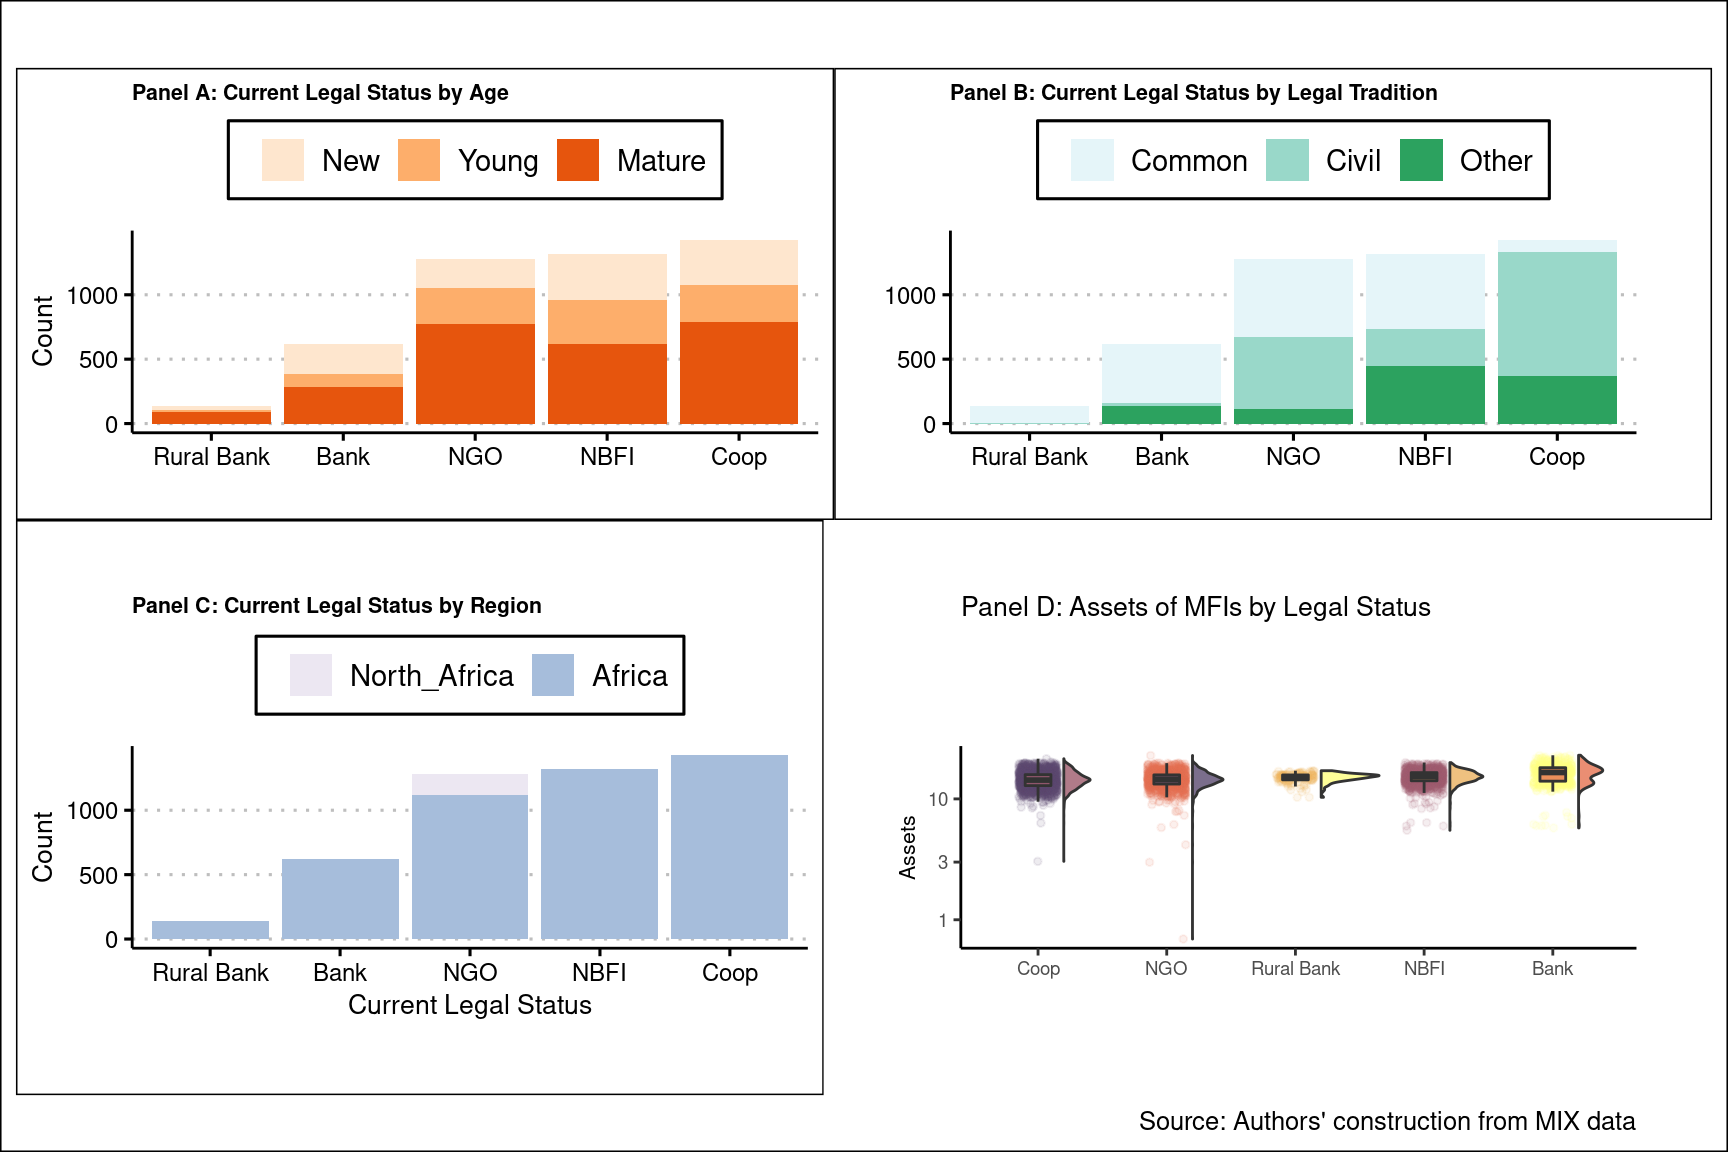
\includegraphics{07-troubleshooting_files/figure-latex/unnamed-chunk-19-1} 

}

\caption{Trends in Capital, Debt, Deposits, and Donations}\label{fig:unnamed-chunk-19}
\end{figure}

\end{landscape}

\begin{Shaded}
\begin{Highlighting}[]
\NormalTok{my\_data }\SpecialCharTok{\%\textgreater{}\%} 
  
  \FunctionTok{select}\NormalTok{(asset\_structure, assets, pcrdbgdp, }
         
\NormalTok{         stmktcap, profit\_margin, }
         
\NormalTok{         pcrdbgdp, stmktcap) }\SpecialCharTok{\%\textgreater{}\%} 
  
  \FunctionTok{skim\_without\_charts}\NormalTok{() }\SpecialCharTok{\%\textgreater{}\%} 
  
  \FunctionTok{mutate}\NormalTok{(}\AttributeTok{N =} \DecValTok{4782}\NormalTok{) }\SpecialCharTok{\%\textgreater{}\%} 
  
  \FunctionTok{select}\NormalTok{(}\SpecialCharTok{{-}}\NormalTok{complete\_rate, }\SpecialCharTok{{-}}\NormalTok{n\_missing, }\SpecialCharTok{{-}}\NormalTok{skim\_type) }\SpecialCharTok{\%\textgreater{}\%} 

  \FunctionTok{rename}\NormalTok{(}\AttributeTok{Variable =}\NormalTok{ skim\_variable, }
         
         \AttributeTok{Mean =}\NormalTok{ numeric.mean, }\AttributeTok{SD =}\NormalTok{ numeric.sd, }
         
         \AttributeTok{Min =}\NormalTok{ numeric.p0, }\AttributeTok{Q1 =}\NormalTok{ numeric.p25,}
         
         \AttributeTok{Median =}\NormalTok{ numeric.p50, }\AttributeTok{Q3 =}\NormalTok{ numeric.p75, }\AttributeTok{Max =}\NormalTok{ numeric.p100) }\SpecialCharTok{\%\textgreater{}\%} 
  
  \FunctionTok{relocate}\NormalTok{(N, }\AttributeTok{.after =}\NormalTok{ Variable) }\SpecialCharTok{\%\textgreater{}\%} 
  
  \FunctionTok{kbl}\NormalTok{(., }\AttributeTok{caption =} \StringTok{"Summary Statistics for Categrical Independent Variables"}\NormalTok{, }
      
      \AttributeTok{booktabs =} \ConstantTok{TRUE}\NormalTok{) }\SpecialCharTok{\%\textgreater{}\%} 
  
  \FunctionTok{kable\_paper}\NormalTok{(}\AttributeTok{full\_width =} \ConstantTok{TRUE}\NormalTok{, }\AttributeTok{font\_size =} \DecValTok{10}\NormalTok{) }\SpecialCharTok{\%\textgreater{}\%} 
  
  \FunctionTok{footnote}\NormalTok{(}\AttributeTok{general =} \StringTok{"Authors\textquotesingle{} construction from the MIX data"}\NormalTok{,}
           
           \AttributeTok{general\_title =} \StringTok{"Source: "}\NormalTok{,}
           
           \AttributeTok{number =} \FunctionTok{c}\NormalTok{(}\StringTok{"Legal status include NGO, Non{-}Bank Financial Institutions (NBFIs), Credit Unions, and Banks"}\NormalTok{, }\StringTok{"Age has mature MFIs older than 8 years, young ones (4 {-} 8 years), and new ones that are 4 years or less"}\NormalTok{),}
           \AttributeTok{number\_title =} \StringTok{"Note: "}\NormalTok{)}
\end{Highlighting}
\end{Shaded}

\begin{table}

\caption{\label{tab:unnamed-chunk-20}Summary Statistics for Categrical Independent Variables}
\centering
\fontsize{10}{12}\selectfont
\begin{tabu} to \linewidth {>{\raggedright}X>{\raggedleft}X>{\raggedleft}X>{\raggedleft}X>{\raggedleft}X>{\raggedleft}X>{\raggedleft}X>{\raggedleft}X>{\raggedleft}X}
\toprule
Variable & N & Mean & SD & Min & Q1 & Median & Q3 & Max\\
\midrule
asset\_structure & 4782 & 0.076 & 0.069 & 0.00e+00 & 0.035 & 0.060 & 0.092 & 0.86\\
assets & 4782 & 14.946 & 2.262 & 6.93e-01 & 13.540 & 14.858 & 16.416 & 22.98\\
pcrdbgdp & 4782 & 2.719 & 0.685 & 2.98e-01 & 2.386 & 2.758 & 3.052 & 6.88\\
stmktcap & 4782 & 1.141 & 1.473 & 0.00e+00 & 0.000 & 0.000 & 2.428 & 5.80\\
profit\_margin & 4782 & -7.739 & 513.299 & -3.55e+04 & -0.181 & 0.048 & 0.189 & 6.20\\
\bottomrule
\multicolumn{9}{l}{\rule{0pt}{1em}\textit{Source: }}\\
\multicolumn{9}{l}{\rule{0pt}{1em}Authors' construction from the MIX data}\\
\multicolumn{9}{l}{\rule{0pt}{1em}\textit{Note: }}\\
\multicolumn{9}{l}{\rule{0pt}{1em}\textsuperscript{1} Legal status include NGO, Non-Bank Financial Institutions (NBFIs), Credit Unions, and Banks}\\
\multicolumn{9}{l}{\rule{0pt}{1em}\textsuperscript{2} Age has mature MFIs older than 8 years, young ones (4 - 8 years), and new ones that are 4 years or less}\\
\end{tabu}
\end{table}

\hypertarget{regression-results}{%
\section{Regression Results}\label{regression-results}}

This section discusses the output from the regression models, starting with the debt to equity ratio, the capital to assets ratio, the deposits to total assets ratio, and the donations to assets ratio. Appendix 1 shows the results of the Hausmann Test and the choice over fixed and random effects models \autocite{clark2015should}. For the Hausmann test, the null hypothesis is for the random-effects model \autocite{torres2007panel}. The results favour the random-effects model, except for the model with debt to equity ratio as the response. For robustness, however, we run both fixed and random effects. The data at hand is an unbalanced panel.

For this reason, we ran a random-effects model on the full dataset. We then subset the data for instances with three or more years of data and then five or more years of data. These figures (three and five) correspond to the mean and median number of years of data per MFI dataset. Finally, we run a pooled OLS and a fixed-effects model using the entire dataset.

\hypertarget{drivers-of-leverage-debt-to-equity-ratio}{%
\subsection{Drivers of Leverage (Debt to Equity Ratio)}\label{drivers-of-leverage-debt-to-equity-ratio}}

Table 3 shows the output of the relevant regression models with debt to equity ratio as the dependent variable. The regressions indicate that MFI age matters the most in determining the debt to equity ratio at the firm level. At the macro-level, institutional quality is a significant driver of leverage.

\textbf{Age:} The regression output for leverage is in Table 5 below. Regarding age, new MFIs (0-4 years) in Africa have a significantly higher debt to equity ratio than young MFIs (4-8 years), on average. However, there is no significant difference between the leverage of new MFIs and mature MFIs (8 years and above), although the coefficient has a negative sign suggesting lower debt to equity ratio. This result means that the oldest firms and the newest MFIs tend to finance their operations with more equity than debt. Given that equity is riskier than debt, it follows that investors have more confidence in older MFIs and youngest MFIs. The capital structure theory does not mention the age of a firm as a significant driver of capital structure. However, suppose age has a direct correspondence with size. In that case, we expect that older, larger MFIs are more profitable (a source of internal equity) and can attract long term equity funding due to their track record \autocite{barclay2005capital,barclay2006debt}. The relatively high debt to equity ratio of new MFIs could reflect the emphasis on the financial sustainability of MFIs which makes start-ups resort to relatively more debt to finance their operations due to reduced availability of donations and government subsidies \autocite{gwatidzo2009corporate}. Without the initial support from donors, equity funders deem start-up MFIs too risky. Without the initial seed capital in grants and concessionary funds, the institutional lifecycle theory of \textcite{bayai2016financing} may not hold.

\textbf{Institutional Quality (KKM):} Institutional quality or governance (KKM) has an inverse relationship with the debt to equity ratio of MFIs in Africa. Higher KKM corresponds to a lower debt to equity ratio and vice versa, implying that MFIs in high KKM countries rely more on equity than debt. Research on capital structure theory shows that indeed governance matters in determining the ease of contract enforcement and safeguarding property rights \autocite{butkiewicz2006institutional}. Governance also reflects the effective regulation of capital markets, hence better capital markets development \autocite{matias2017there,ombati2016effects}. In MFIs, better KKM may encourage long term equity investment relative to debt investment and thus the observed relationship.

\begin{landscape}

\begin{Shaded}
\begin{Highlighting}[]
\DocumentationTok{\#\#\#\#\#\#\#\#\#\#\#\#\#\#\#\#\#\#\#\#\#\#\#\#}
\NormalTok{fixed\_effects\_de }\OtherTok{\textless{}{-}} \FunctionTok{modelling}\NormalTok{(}\AttributeTok{data =}\NormalTok{ my\_data, }\AttributeTok{depvar =}\NormalTok{ my\_data}\SpecialCharTok{$}\NormalTok{debt\_to\_equity\_ratio)}

\NormalTok{fixed\_effects\_de3 }\OtherTok{\textless{}{-}} \FunctionTok{modelling}\NormalTok{(}\AttributeTok{data =}\NormalTok{ data3, }\AttributeTok{depvar =}\NormalTok{ data3}\SpecialCharTok{$}\NormalTok{debt\_to\_equity\_ratio)}

\NormalTok{fixed\_effects\_de5 }\OtherTok{\textless{}{-}} \FunctionTok{modelling}\NormalTok{(}\AttributeTok{data =}\NormalTok{ data5, }\AttributeTok{depvar =}\NormalTok{ data5}\SpecialCharTok{$}\NormalTok{debt\_to\_equity\_ratio)}

\NormalTok{random\_effects\_de }\OtherTok{\textless{}{-}} \FunctionTok{modelling}\NormalTok{(}\AttributeTok{data =}\NormalTok{ my\_data, }\AttributeTok{depvar =}\NormalTok{ my\_data}\SpecialCharTok{$}\NormalTok{debt\_to\_equity\_ratio, }\AttributeTok{model =} \StringTok{"random"}\NormalTok{)}

\NormalTok{random\_effects\_de3 }\OtherTok{\textless{}{-}} \FunctionTok{modelling}\NormalTok{(}\AttributeTok{data =}\NormalTok{ data3, }\AttributeTok{depvar =}\NormalTok{ data3}\SpecialCharTok{$}\NormalTok{debt\_to\_equity\_ratio, }\AttributeTok{model =} \StringTok{"random"}\NormalTok{)}

\NormalTok{random\_effects\_de5 }\OtherTok{\textless{}{-}} \FunctionTok{modelling}\NormalTok{(}\AttributeTok{data =}\NormalTok{ data5, }\AttributeTok{depvar =}\NormalTok{ data5}\SpecialCharTok{$}\NormalTok{debt\_to\_equity\_ratio, }\AttributeTok{model =} \StringTok{"random"}\NormalTok{)}

\NormalTok{pooling\_de }\OtherTok{\textless{}{-}} \FunctionTok{modelling}\NormalTok{(}\AttributeTok{data =}\NormalTok{ my\_data, }\AttributeTok{depvar =}\NormalTok{ my\_data}\SpecialCharTok{$}\NormalTok{debt\_to\_equity\_ratio, }\AttributeTok{model =} \StringTok{"pooling"}\NormalTok{)}

\DocumentationTok{\#\#\#\#\#\#\#\#\#\#\#\#\#\#\#\#\#\#\#\#\#\#\#\#\#\#\#\#\#\#\#\#\#\#\#\#\#\#\#\#\#\#\#\#\#\#\#\#\#\#\#\#\#}

\NormalTok{inference\_m101 }\OtherTok{\textless{}{-}} \FunctionTok{coeftest}\NormalTok{(fixed\_effects\_de, }\AttributeTok{vcov =} \FunctionTok{vcovBK}\NormalTok{(fixed\_effects\_de, }\AttributeTok{method =} \StringTok{"arellano"}\NormalTok{, }\AttributeTok{type=}\StringTok{"HC1"}\NormalTok{, }\AttributeTok{cluster =} \StringTok{"group"}\NormalTok{))}

\NormalTok{inference\_m111 }\OtherTok{\textless{}{-}} \FunctionTok{coeftest}\NormalTok{(fixed\_effects\_de3, }\AttributeTok{vcov =} \FunctionTok{vcovBK}\NormalTok{(fixed\_effects\_de3, }\AttributeTok{method =} \StringTok{"arellano"}\NormalTok{, }\AttributeTok{type=}\StringTok{"HC1"}\NormalTok{, }\AttributeTok{cluster =} \StringTok{"group"}\NormalTok{))}

\NormalTok{inference\_m121 }\OtherTok{\textless{}{-}} \FunctionTok{coeftest}\NormalTok{(fixed\_effects\_de5 , }\AttributeTok{vcov =} \FunctionTok{vcovBK}\NormalTok{(fixed\_effects\_de5 , }\AttributeTok{method =} \StringTok{"arellano"}\NormalTok{, }\AttributeTok{type=}\StringTok{"HC1"}\NormalTok{, }\AttributeTok{cluster =} \StringTok{"group"}\NormalTok{))}

\NormalTok{inference\_m131 }\OtherTok{\textless{}{-}} \FunctionTok{coeftest}\NormalTok{(random\_effects\_de, }\AttributeTok{vcov =} \FunctionTok{vcovBK}\NormalTok{(random\_effects\_de, }\AttributeTok{method =} \StringTok{"arellano"}\NormalTok{, }\AttributeTok{type=}\StringTok{"HC1"}\NormalTok{, }\AttributeTok{cluster =} \StringTok{"group"}\NormalTok{))}

\NormalTok{inference\_m141 }\OtherTok{\textless{}{-}} \FunctionTok{coeftest}\NormalTok{(random\_effects\_de3, }\AttributeTok{vcov =} \FunctionTok{vcovBK}\NormalTok{(random\_effects\_de3, }\AttributeTok{method =} \StringTok{"arellano"}\NormalTok{, }\AttributeTok{type=}\StringTok{"HC1"}\NormalTok{, }\AttributeTok{cluster =} \StringTok{"group"}\NormalTok{))}

\NormalTok{inference\_m151 }\OtherTok{\textless{}{-}} \FunctionTok{coeftest}\NormalTok{(random\_effects\_de5, }\AttributeTok{vcov =} \FunctionTok{vcovBK}\NormalTok{(random\_effects\_de5, }\AttributeTok{method =} \StringTok{"arellano"}\NormalTok{, }\AttributeTok{type=}\StringTok{"HC1"}\NormalTok{, }\AttributeTok{cluster =} \StringTok{"group"}\NormalTok{))}


\DocumentationTok{\#\#\#\#\#\#\#\#\#\#\#\#\#\#\#\#\#\#\#\#\#\#\#\#\#\#\#\#\#\#\#\#\#\#\#\#\#\#\#\#\#\#\#\#\#\#\#\#\#\#\#\#}

\FunctionTok{stargazer}\NormalTok{(fixed\_effects\_de, fixed\_effects\_de3, }
          
\NormalTok{          fixed\_effects\_de5, random\_effects\_de, random\_effects\_de3, random\_effects\_de5,}
          
          \AttributeTok{se =} \FunctionTok{list}\NormalTok{(inference\_m101[,}\DecValTok{2}\NormalTok{], inference\_m111[,}\DecValTok{2}\NormalTok{], inference\_m121[,}\DecValTok{2}\NormalTok{], }
          
\NormalTok{          inference\_m131[,}\DecValTok{2}\NormalTok{], inference\_m141[,}\DecValTok{2}\NormalTok{], inference\_m151[,}\DecValTok{2}\NormalTok{]),}
          
          \AttributeTok{title =} \StringTok{"Regression Output for Debt to Equity Ratio (Standard Errors in Brackets)"}\NormalTok{, }
          
          \AttributeTok{align =} \ConstantTok{TRUE}\NormalTok{, }\AttributeTok{font.size =} \StringTok{"tiny"}\NormalTok{, }\AttributeTok{header =} \ConstantTok{FALSE}\NormalTok{, }
          
          \AttributeTok{omit =} \FunctionTok{c}\NormalTok{(}\StringTok{"year."}\NormalTok{, }\StringTok{"Constant"}\NormalTok{),}
          
          \AttributeTok{add.lines =} \FunctionTok{list}\NormalTok{(}\FunctionTok{c}\NormalTok{(}\StringTok{"Model"}\NormalTok{, }\StringTok{"Within"}\NormalTok{, }\StringTok{"Within"}\NormalTok{, }\StringTok{"Within"}\NormalTok{, }
                        
                        \StringTok{"Random"}\NormalTok{, }\StringTok{"Random"}\NormalTok{, }\StringTok{"Random"}\NormalTok{), }
          
          \FunctionTok{c}\NormalTok{(}\StringTok{"Data"}\NormalTok{, }\StringTok{"Full"}\NormalTok{, }\StringTok{"\textgreater{}=3 Years"}\NormalTok{, }\StringTok{"\textgreater{}=5 Years"}\NormalTok{, }
            
            \StringTok{"Full"}\NormalTok{, }\StringTok{"\textgreater{}=3 Years"}\NormalTok{, }\StringTok{"\textgreater{}=5 Years"}\NormalTok{)))}
\end{Highlighting}
\end{Shaded}

\begin{table}[!htbp] \centering 
  \caption{Regression Output for Debt to Equity Ratio (Standard Errors in Brackets)} 
  \label{} 
\tiny 
\begin{tabular}{@{\extracolsep{5pt}}lD{.}{.}{-3} D{.}{.}{-3} D{.}{.}{-3} D{.}{.}{-3} D{.}{.}{-3} D{.}{.}{-3} } 
\\[-1.8ex]\hline 
\hline \\[-1.8ex] 
 & \multicolumn{6}{c}{\textit{Dependent variable:}} \\ 
\cline{2-7} 
\\[-1.8ex] & \multicolumn{6}{c}{depvar} \\ 
\\[-1.8ex] & \multicolumn{1}{c}{(1)} & \multicolumn{1}{c}{(2)} & \multicolumn{1}{c}{(3)} & \multicolumn{1}{c}{(4)} & \multicolumn{1}{c}{(5)} & \multicolumn{1}{c}{(6)}\\ 
\hline \\[-1.8ex] 
 currentlegalstatusBank &  &  &  & -0.957 & -1.840 & -0.045 \\ 
  &  &  &  & (3.210) & (4.240) & (2.360) \\ 
  & & & & & & \\ 
 currentlegalstatusNBFI &  &  &  & -0.439 & -1.580 & -0.796 \\ 
  &  &  &  & (2.810) & (3.450) & (1.790) \\ 
  & & & & & & \\ 
 currentlegalstatusCoop & 6.450 & 6.990 & 5.840 & -2.290 & -4.760 & 0.453 \\ 
  & (24.400) & (27.300) & (40.200) & (2.710) & (3.480) & (2.060) \\ 
  & & & & & & \\ 
 currentlegalstatusRural Bank &  &  &  & 2.280 & 1.190 & -0.868 \\ 
  &  &  &  & (8.690) & (12.400) & (4.630) \\ 
  & & & & & & \\ 
 ageYoung & -7.130^{*} & -9.220^{**} & -1.630 & -4.480 & -6.680^{*} & -2.080 \\ 
  & (3.830) & (4.360) & (2.300) & (2.850) & (3.810) & (2.260) \\ 
  & & & & & & \\ 
 ageMature & -3.220 & -4.570 & 0.235 & -0.547 & -1.490 & -1.240 \\ 
  & (3.940) & (4.440) & (2.510) & (2.350) & (3.410) & (2.110) \\ 
  & & & & & & \\ 
 legal\_traditionCivil &  &  &  & -0.605 & -1.320 & -0.803 \\ 
  &  &  &  & (3.400) & (4.360) & (2.210) \\ 
  & & & & & & \\ 
 legal\_traditionOther &  &  &  & 0.926 & 1.560 & -0.495 \\ 
  &  &  &  & (3.240) & (4.220) & (2.470) \\ 
  & & & & & & \\ 
 kkm & -4.080^{**} & -4.740^{**} & -1.140 & -0.299 & -0.472 & -0.821^{*} \\ 
  & (1.700) & (1.880) & (0.936) & (0.520) & (0.704) & (0.421) \\ 
  & & & & & & \\ 
 asset\_structure & -10.100 & -13.200 & -8.260 & -10.300 & -13.900 & -17.900 \\ 
  & (28.800) & (33.200) & (20.600) & (11.800) & (17.400) & (12.000) \\ 
  & & & & & & \\ 
 pcrdbgdp & -0.724 & -0.939 & 0.848 & -1.540 & -2.130 & -0.701 \\ 
  & (3.940) & (4.570) & (2.990) & (1.780) & (2.260) & (1.310) \\ 
  & & & & & & \\ 
 stmktcap & 0.229 & 0.239 & -0.552 & 0.831 & 0.627 & 0.090 \\ 
  & (3.130) & (3.370) & (2.000) & (0.984) & (1.280) & (0.754) \\ 
  & & & & & & \\ 
 profit\_margin & 0.00001 & -0.00002 & 0.265 & 0.00001 & -0.00001 & 0.173 \\ 
  & (0.002) & (0.002) & (0.295) & (0.001) & (0.001) & (0.258) \\ 
  & & & & & & \\ 
\hline \\[-1.8ex] 
Model & Within & Within & Within & Random & Random & Random \\ 
Data & Full & >=3 Years & >=5 Years & Full & >=3 Years & >=5 Years \\ 
Observations & \multicolumn{1}{c}{4,782} & \multicolumn{1}{c}{3,840} & \multicolumn{1}{c}{3,165} & \multicolumn{1}{c}{4,782} & \multicolumn{1}{c}{3,840} & \multicolumn{1}{c}{3,165} \\ 
R$^{2}$ & \multicolumn{1}{c}{0.006} & \multicolumn{1}{c}{0.009} & \multicolumn{1}{c}{0.005} & \multicolumn{1}{c}{0.005} & \multicolumn{1}{c}{0.007} & \multicolumn{1}{c}{0.007} \\ 
Adjusted R$^{2}$ & \multicolumn{1}{c}{-0.230} & \multicolumn{1}{c}{-0.131} & \multicolumn{1}{c}{-0.106} & \multicolumn{1}{c}{-0.002} & \multicolumn{1}{c}{-0.002} & \multicolumn{1}{c}{-0.003} \\ 
F Statistic & \multicolumn{1}{c}{0.878 (df = 28; 3862)} & \multicolumn{1}{c}{1.040 (df = 28; 3366)} & \multicolumn{1}{c}{0.557 (df = 28; 2845)} & \multicolumn{1}{c}{24.600} & \multicolumn{1}{c}{26.500} & \multicolumn{1}{c}{23.500} \\ 
\hline 
\hline \\[-1.8ex] 
\textit{Note:}  & \multicolumn{6}{r}{$^{*}$p$<$0.1; $^{**}$p$<$0.05; $^{***}$p$<$0.01} \\ 
\end{tabular} 
\end{table}

\end{landscape}

\hypertarget{drivers-of-capital-to-assets-ratio-in-microfinance-institutions}{%
\subsection{Drivers of Capital to Assets Ratio in Microfinance Institutions}\label{drivers-of-capital-to-assets-ratio-in-microfinance-institutions}}

Regression results for the drivers of the capital-assets ratio among MFIs in Africa appear in Table 4. Capital assets ratio is the ratio of total equity to total assets. Again, legal status, age, legal tradition, and stock market development are related to the equity to total assets ratio. We examine these significant variables in turn.

\textbf{Current Legal Status:} NGOs consistently have higher capital to assets ratio than other legal traditions: banks, cooperatives, NBFIs, and rural banks. The definition of debt to equity ratio means that NGOs finance their operations using more equity than debt. The results align with the institutional life cycle theory, which posits that MFIs often start financing operations using donations and concessionary funds, then switch to equity as they mature \autocite{bayai2016financing}. Debt is often for well established MFIs, at which point they are likely financially sustainable and likely to switch to the commercial model \autocite{d2017ngos}. NBFIs have the second-highest mean and median levels of capital to assets ratio, followed by banks, while cooperative and rural banks come last in that order. These results align with the literature confirming the high leverage of banks \autocite{mettenheim2013back}, with the bulk of the capital in deposits.

The results also reflect the market conditions where donations and subsidies are getting less available as donors begin to stress sustainability. Mature firms have a long-running relationship with donors to the extent they have a profitable business model and developed a business profile that allows them to make profits and issue equity. Characteristically, commercial banks and other deposit-taking institutions tend to be more leveraged than other financial intermediaries because they have the license and scale to garner deposits and other debt instruments, explaining the pattern of results.

\textbf{Age:} The capital to asset ratio of MFIs in Africa decreases with age. Young (4-8 years) and mature (8 years and over) MFIs have lower capital to assets ratios, on average than new MFIs (0-4 years). The mean and median capital to assets ratio These results are also in line with the literature on capital structure. Older firms are likely larger with more support to pledge as collateral and quickly raise funds in the debt markets \autocite{barclay2005capital}. Also, as MFIs mature, they are likely to graduate from the loans only model to start accepting deposits which further raises their leverage. Overall, this makes the equity component smaller relative to the debt component. In the capital structure literature, age is not a significant driver of the capital structure except through its link to the size of an MFI, as we discuss next.

\textbf{Legal Tradition:} MFIs located in common law countries have, on average, higher capital to assets ratio than equivalent MFIs in civil law or other legal tradition countries. The results follow from the law and finance literature, showing that common law legal tradition corresponds to a higher level of capital market development, especially stock market development \autocite{la2013law}. Civil law countries have the lowest mean and median capital to assets ratio confirming the law and finance literature in Africa's context \autocite{schnyder2018twenty}. If capital markets and especially equity markets are more developed in common law countries, it means that MFIs can quickly issue equity financial instruments. Also, venture capitalists are more willing to inject private equity in MFIs in common law countries. The public equity markets offer an opportunity to exit the investment once it takes root \autocite{kent2013bankers}.

\textbf{Stock Market Development:} There is a weak negative but statistically significant relationship between stock market development and capital to assets ratio. It means that MFIs in countries with vulnerable stock markets have more equity relative to assets and vice versa. These results may reflect the bank-based versus capital market-based model of financing. Most economies in Africa follow the bank-based model \autocite{gropp2010determinants}, where firms mainly raise funds from commercial banks in loans instead of equity and debt markets. Effectively, there is a weak link between microfinance and the equity and debt market, reflecting the small coefficients \autocite{ahmed2014financial}. MFIs appear to have little linkage with the equity markets, and even where they do, prefer retained earnings and private equity to listing publicly. Available evidence shows very few cases of MFIs that are publicly listed \autocite{hishigsuren2006transformation}.

\textbf{Other Insignificant Variables:} Governance or institutional quality (KKM), asset structure, private credit to GDP, and profit margin are statistically insignificant capital to assets ratio drivers. However, KKM and private credit to GDP both have a positive relationship with capital to assets ratio, reflecting the importance of institutions both in the development of debt and equity markets. The relationship between assets structure and profit margin on the one hand, and capital to assets ratio on the other, shows mixed results, which may highlight the low profitability of MFIs in Africa (see appendix 7).

\hypertarget{drivers-of-deposits-to-total-assets}{%
\subsection{Drivers of Deposits to Total Assets}\label{drivers-of-deposits-to-total-assets}}

The deposits to assets ratio have a positive relationship with MFI legal form, age, asset structure, size (logarithm of assets), and profit margin. The significant drivers of the deposits to assets ratio at the macro-level are legal tradition and institutional quality (KKM). Proxies for capital markets development, private credit to GDP and stock markets development to GDP do not significantly affect deposits to assets ratio. We discuss each of these relationships next.

\textbf{Current Legal Status:} NGO-type MFIs have lower deposits to assets ratio than commercial banks, credit unions/ cooperatives, NBFIs, and rural banks. These results arise out of the different business models. NGOs have taken root dependent on donations and subsidies with little emphasis on deposit mobilisation \autocite{d2013unsubsidized,d2017ngos}. For instance, Credit Unions, on the other hand, thrive on taking deposits from members who raise their capacity for deposits mobilisation compared to NGOs. For NGOs, the lower deposits to assets ratio could be due to legal restrictions on deposit mobilisation by entities not under central banks' oversight \autocite{lauer2008transforming}. As expected, rural banks, commercial banks and cooperatives have the highest mean and median deposits to assets ratios. Commercial banks and Credit Unions thrive on taking deposits from members who raise their capacity for deposits mobilisation compared to commercial banks, reflecting their high deposits-driven leverage levels \autocite{abbas2020commercial}.

\textbf{Age:} Older MFIs have higher deposits to assets ratio than younger MFIs. This result reflects the more comprehensive regional presence of older, larger MFIs, which aligns with the capital structure theory \autocite{barclay2005capital,barclay2006debt} and enhanced goodwill from the public. Also, older MFIs have invested in information technology to reach people in remote locations \autocite{di2021technology}. Again, older MFIs are likely to have attained deposit mobilisation licenses from relevant regulatory bodies like central banks. The results are in line with capital structure theory, where the size of an MFI, which is also positively related to age, has a significant relationship with leverage. For most financial intermediaries, the largest deposits are the largest source of debt financing \autocite{gale2020bank}.

\textbf{Legal Tradition:} MFIs in countries with civil law and other legal traditions tend to have a higher deposit to assets ratio than those in common law countries, with MFIs in civil law countries having the highest proportion. It means that MFIs in common law countries finance their operations using more equity than civil law countries. These results are in line with the higher levels of capital markets development in common law countries \autocite{la2013law,schnyder2018twenty} that allows MFIs to quickly raise equity capital and debt capital in a form other than deposits.

\textbf{Institutional Quality (KKM):} The institutional quality or governance (KKM) has a weak negative relationship with the deposits to assets ratio, holding all other variables constant. In other words, MFIs located in countries with better governance rely less on deposits and more on alternative forms of finance, namely equity and debt, than MFIs with lower governance metrics. These results would imply that as institutional quality improves, people are less likely to maintain deposits, and instead, prefer the capital markets and other sorts of investments. The argument will hold if KKM supports the development of financial and other markets that facilitates investments with better returns than bank deposits offer \autocite{la2013law,schnyder2018twenty}. Indeed, although primarily insignificant, the degree of capital market development has a negative relationship with the deposits to assets ratio, which could render credence to the argument. Also, with better-developed capital markets, MFIs can access finance from other sources, lowering the relative importance of deposits.

\textbf{Asset Structure:} Asset structure or asset tangibility has a mixed relationship with deposits to assets ratio, ceteris paribus. However, capital structure theory shows that firms can use tangible assets as collateral for debt funding. Thus, firms with more tangible assets usually have more debt at a lower cost than firms with less tangible assets \autocite{campello2011capital,ombati2016effects}. However, the rise of information technology means that MFIs no longer have to hold high tangible (fixed) assets, especially in property, plant and equipment, to reach the unbanked population \autocite{asadullah2021access}. Except for older firms that had already invested in many branches before information technology took root, asset structure is likely insignificant in deposits mobilisation \autocite{di2021technology}.

\textbf{Profit Margin:} Profit margin has a positive but very weak positive relationship with deposits to assets ratio. The result could hold that profitable MFIs reach more consumers by opening more branches or investing more in information technology \autocite{di2021technology}. Moreover, in line with the capital structure theory, Profitable firms are usually large and mature with free cash flows to support debt repayment and thus hold more debt. Firms take up debt to minimise cash that managers could misallocate. The debtholders act as delegated monitors and further monitor management \autocite{barclay2005capital,gwatidzo2009corporate,ombati2016effects}. Finally, both stock market capitalisation to GDP and private credit to GDP has no significant effect on the deposits to assets ratio.

\begin{landscape}

\begin{Shaded}
\begin{Highlighting}[]
\DocumentationTok{\#\#\#\#\#\#\#\#\#\#\#\#\#\#\#\#\#\#\#\#\#\#\#\#\#\#\#\#\#\#\#\#\#\#\#\#\#}
\NormalTok{fixed\_effects\_car }\OtherTok{\textless{}{-}} \FunctionTok{modelling}\NormalTok{(}\AttributeTok{data =}\NormalTok{ my\_data, }\AttributeTok{depvar =}\NormalTok{ my\_data}\SpecialCharTok{$}\NormalTok{capital\_asset\_ratio)}

\NormalTok{fixed\_effects\_car3 }\OtherTok{\textless{}{-}} \FunctionTok{modelling}\NormalTok{(}\AttributeTok{data =}\NormalTok{ data3, }\AttributeTok{depvar =}\NormalTok{ data3}\SpecialCharTok{$}\NormalTok{capital\_asset\_ratio)}

\NormalTok{fixed\_effects\_car5 }\OtherTok{\textless{}{-}} \FunctionTok{modelling}\NormalTok{(}\AttributeTok{data =}\NormalTok{ data5, }\AttributeTok{depvar =}\NormalTok{ data5}\SpecialCharTok{$}\NormalTok{capital\_asset\_ratio)}

\NormalTok{random\_effects\_car }\OtherTok{\textless{}{-}} \FunctionTok{modelling}\NormalTok{(}\AttributeTok{data =}\NormalTok{ my\_data, }\AttributeTok{depvar =}\NormalTok{ my\_data}\SpecialCharTok{$}\NormalTok{capital\_asset\_ratio, }\AttributeTok{model =} \StringTok{"random"}\NormalTok{)}

\NormalTok{random\_effects\_car3 }\OtherTok{\textless{}{-}} \FunctionTok{modelling}\NormalTok{(}\AttributeTok{data =}\NormalTok{ data3, }\AttributeTok{depvar =}\NormalTok{ data3}\SpecialCharTok{$}\NormalTok{capital\_asset\_ratio, }\AttributeTok{model =} \StringTok{"random"}\NormalTok{)}

\NormalTok{random\_effects\_car5 }\OtherTok{\textless{}{-}} \FunctionTok{modelling}\NormalTok{(}\AttributeTok{data =}\NormalTok{ data5, }\AttributeTok{depvar =}\NormalTok{ data5}\SpecialCharTok{$}\NormalTok{capital\_asset\_ratio, }\AttributeTok{model =} \StringTok{"random"}\NormalTok{)}

\NormalTok{pooling\_car }\OtherTok{\textless{}{-}} \FunctionTok{modelling}\NormalTok{(}\AttributeTok{data =}\NormalTok{ my\_data, }\AttributeTok{depvar =}\NormalTok{ my\_data}\SpecialCharTok{$}\NormalTok{capital\_asset\_ratio, }\AttributeTok{model =} \StringTok{"pooling"}\NormalTok{)}

\DocumentationTok{\#\#\#\#\#\#\#\#\#\#\#\#\#\#\#\#\#\#\#\#\#\#\#\#\#\#\#\#\#\#\#\#\#\#\#\#\#\#\#\#\#\#\#\#\#\#}
\NormalTok{inference\_m201 }\OtherTok{\textless{}{-}} \FunctionTok{coeftest}\NormalTok{(fixed\_effects\_car, }\AttributeTok{vcov =} \FunctionTok{vcovBK}\NormalTok{(fixed\_effects\_car, }\AttributeTok{method =} \StringTok{"arellano"}\NormalTok{, }\AttributeTok{type=}\StringTok{"HC1"}\NormalTok{, }\AttributeTok{cluster =} \StringTok{"group"}\NormalTok{))}

\NormalTok{inference\_m211 }\OtherTok{\textless{}{-}} \FunctionTok{coeftest}\NormalTok{(fixed\_effects\_car3, }\AttributeTok{vcov =} \FunctionTok{vcovBK}\NormalTok{(fixed\_effects\_car3, }\AttributeTok{method =} \StringTok{"arellano"}\NormalTok{, }\AttributeTok{type=}\StringTok{"HC1"}\NormalTok{, }\AttributeTok{cluster =} \StringTok{"group"}\NormalTok{))}

\NormalTok{inference\_m221 }\OtherTok{\textless{}{-}} \FunctionTok{coeftest}\NormalTok{(fixed\_effects\_car5 , }\AttributeTok{vcov =} \FunctionTok{vcovBK}\NormalTok{(fixed\_effects\_car, }\AttributeTok{method =} \StringTok{"arellano"}\NormalTok{, }\AttributeTok{type=}\StringTok{"HC1"}\NormalTok{, }\AttributeTok{cluster =} \StringTok{"group"}\NormalTok{))}

\NormalTok{inference\_m231 }\OtherTok{\textless{}{-}} \FunctionTok{coeftest}\NormalTok{(random\_effects\_car, }\AttributeTok{vcov =} \FunctionTok{vcovBK}\NormalTok{(random\_effects\_car, }\AttributeTok{method =} \StringTok{"arellano"}\NormalTok{, }\AttributeTok{type=}\StringTok{"HC1"}\NormalTok{, }\AttributeTok{cluster =} \StringTok{"group"}\NormalTok{))}

\NormalTok{inference\_m241 }\OtherTok{\textless{}{-}} \FunctionTok{coeftest}\NormalTok{(random\_effects\_car3, }\AttributeTok{vcov =} \FunctionTok{vcovBK}\NormalTok{(random\_effects\_car3, }\AttributeTok{method =} \StringTok{"arellano"}\NormalTok{, }\AttributeTok{type=}\StringTok{"HC1"}\NormalTok{, }\AttributeTok{cluster =} \StringTok{"group"}\NormalTok{))}

\NormalTok{inference\_m251 }\OtherTok{\textless{}{-}} \FunctionTok{coeftest}\NormalTok{(random\_effects\_car5, }\AttributeTok{vcov =} \FunctionTok{vcovBK}\NormalTok{(random\_effects\_car5, }\AttributeTok{method =} \StringTok{"arellano"}\NormalTok{, }\AttributeTok{type=}\StringTok{"HC1"}\NormalTok{, }\AttributeTok{cluster =} \StringTok{"group"}\NormalTok{))}


\DocumentationTok{\#\#\#\#\#\#\#\#\#\#\#\#\#\#\#\#\#\#\#\#\#\#\#\#\#\#\#\#\#\#\#\#\#\#\#\#\#\#\#\#\#\#\#\#\#\#}

\FunctionTok{stargazer}\NormalTok{(fixed\_effects\_car, fixed\_effects\_car3, }
          
\NormalTok{          fixed\_effects\_car5, random\_effects\_car, random\_effects\_car3, random\_effects\_car5,}
          
          \AttributeTok{title =} \StringTok{"Regression Output for Capital to Assets Ratio (Standard Errors in Brackets)"}\NormalTok{, }
          
          \AttributeTok{align =} \ConstantTok{TRUE}\NormalTok{, }\AttributeTok{font.size =} \StringTok{"tiny"}\NormalTok{, }\AttributeTok{header =} \ConstantTok{FALSE}\NormalTok{, }
          
          \AttributeTok{se =} \FunctionTok{list}\NormalTok{(inference\_m201[,}\DecValTok{2}\NormalTok{], inference\_m211[,}\DecValTok{2}\NormalTok{], inference\_m221[,}\DecValTok{2}\NormalTok{], }
          
\NormalTok{          inference\_m231[,}\DecValTok{2}\NormalTok{], inference\_m241[,}\DecValTok{2}\NormalTok{], inference\_m251[,}\DecValTok{2}\NormalTok{]),}
          
          \AttributeTok{omit =} \FunctionTok{c}\NormalTok{(}\StringTok{"year."}\NormalTok{, }\StringTok{"Constant"}\NormalTok{),}
          
          \AttributeTok{add.lines =} \FunctionTok{list}\NormalTok{(}\FunctionTok{c}\NormalTok{(}\StringTok{"Model"}\NormalTok{, }\StringTok{"Within"}\NormalTok{, }\StringTok{"Within"}\NormalTok{, }\StringTok{"Within"}\NormalTok{, }
                        
                        \StringTok{"Random"}\NormalTok{, }\StringTok{"Random"}\NormalTok{, }\StringTok{"Random"}\NormalTok{), }
          
          \FunctionTok{c}\NormalTok{(}\StringTok{"Data"}\NormalTok{, }\StringTok{"Full"}\NormalTok{, }\StringTok{"\textgreater{}=3 Years"}\NormalTok{, }\StringTok{"\textgreater{}=5 Years"}\NormalTok{, }
            
            \StringTok{"Full"}\NormalTok{, }\StringTok{"\textgreater{}=3 Years"}\NormalTok{, }\StringTok{"\textgreater{}=5 Years"}\NormalTok{)))}
\end{Highlighting}
\end{Shaded}

\begin{table}[!htbp] \centering 
  \caption{Regression Output for Capital to Assets Ratio (Standard Errors in Brackets)} 
  \label{} 
\tiny 
\begin{tabular}{@{\extracolsep{5pt}}lD{.}{.}{-3} D{.}{.}{-3} D{.}{.}{-3} D{.}{.}{-3} D{.}{.}{-3} D{.}{.}{-3} } 
\\[-1.8ex]\hline 
\hline \\[-1.8ex] 
 & \multicolumn{6}{c}{\textit{Dependent variable:}} \\ 
\cline{2-7} 
\\[-1.8ex] & \multicolumn{6}{c}{depvar} \\ 
\\[-1.8ex] & \multicolumn{1}{c}{(1)} & \multicolumn{1}{c}{(2)} & \multicolumn{1}{c}{(3)} & \multicolumn{1}{c}{(4)} & \multicolumn{1}{c}{(5)} & \multicolumn{1}{c}{(6)}\\ 
\hline \\[-1.8ex] 
 currentlegalstatusBank &  &  &  & -0.201^{***} & -0.157^{***} & -0.162^{***} \\ 
  &  &  &  & (0.064) & (0.047) & (0.047) \\ 
  & & & & & & \\ 
 currentlegalstatusNBFI &  &  &  & -0.047 & -0.055 & -0.082^{**} \\ 
  &  &  &  & (0.053) & (0.037) & (0.035) \\ 
  & & & & & & \\ 
 currentlegalstatusCoop & -0.029 & -0.030 & -0.018 & -0.230^{***} & -0.180^{***} & -0.141^{***} \\ 
  & (0.261) & (0.260) & (0.261) & (0.053) & (0.038) & (0.038) \\ 
  & & & & & & \\ 
 currentlegalstatusRural Bank &  &  &  & -0.277^{***} & -0.304^{***} & -0.319^{***} \\ 
  &  &  &  & (0.092) & (0.087) & (0.113) \\ 
  & & & & & & \\ 
 ageYoung & -0.056^{**} & -0.058^{***} & -0.052^{**} & -0.062^{**} & -0.063^{***} & -0.054^{**} \\ 
  & (0.023) & (0.020) & (0.023) & (0.025) & (0.020) & (0.025) \\ 
  & & & & & & \\ 
 ageMature & -0.072^{**} & -0.073^{***} & -0.062^{**} & -0.068^{**} & -0.077^{***} & -0.069^{**} \\ 
  & (0.029) & (0.028) & (0.029) & (0.028) & (0.025) & (0.028) \\ 
  & & & & & & \\ 
 legal\_traditionCivil &  &  &  & -0.262^{***} & -0.176^{***} & -0.149^{***} \\ 
  &  &  &  & (0.059) & (0.043) & (0.042) \\ 
  & & & & & & \\ 
 legal\_traditionOther &  &  &  & -0.170^{***} & -0.117^{***} & -0.001 \\ 
  &  &  &  & (0.058) & (0.044) & (0.043) \\ 
  & & & & & & \\ 
 kkm & 0.007 & 0.006 & 0.005 & 0.022^{***} & 0.005 & -0.001 \\ 
  & (0.012) & (0.011) & (0.012) & (0.008) & (0.007) & (0.007) \\ 
  & & & & & & \\ 
 asset\_structure & -0.198 & -0.099 & 0.301^{*} & -0.171 & -0.250^{*} & 0.197 \\ 
  & (0.162) & (0.167) & (0.162) & (0.150) & (0.145) & (0.158) \\ 
  & & & & & & \\ 
 pcrdbgdp & 0.026 & 0.027 & 0.024 & 0.009 & 0.018 & 0.019 \\ 
  & (0.035) & (0.031) & (0.035) & (0.028) & (0.019) & (0.020) \\ 
  & & & & & & \\ 
 stmktcap & -0.028 & -0.029 & -0.030 & -0.048^{***} & -0.044^{***} & -0.020 \\ 
  & (0.021) & (0.020) & (0.021) & (0.016) & (0.013) & (0.012) \\ 
  & & & & & & \\ 
 profit\_margin & -0.00000 & -0.00001 & 0.001^{***} & -0.00000 & -0.00001 & 0.002 \\ 
  & (0.00001) & (0.00001) & (0.00001) & (0.00002) & (0.00001) & (0.003) \\ 
  & & & & & & \\ 
\hline \\[-1.8ex] 
Model & Within & Within & Within & Random & Random & Random \\ 
Data & Full & >=3 Years & >=5 Years & Full & >=3 Years & >=5 Years \\ 
Observations & \multicolumn{1}{c}{4,782} & \multicolumn{1}{c}{3,840} & \multicolumn{1}{c}{3,165} & \multicolumn{1}{c}{4,782} & \multicolumn{1}{c}{3,840} & \multicolumn{1}{c}{3,165} \\ 
R$^{2}$ & \multicolumn{1}{c}{0.027} & \multicolumn{1}{c}{0.048} & \multicolumn{1}{c}{0.052} & \multicolumn{1}{c}{0.034} & \multicolumn{1}{c}{0.061} & \multicolumn{1}{c}{0.066} \\ 
Adjusted R$^{2}$ & \multicolumn{1}{c}{-0.205} & \multicolumn{1}{c}{-0.086} & \multicolumn{1}{c}{-0.054} & \multicolumn{1}{c}{0.028} & \multicolumn{1}{c}{0.053} & \multicolumn{1}{c}{0.056} \\ 
F Statistic & \multicolumn{1}{c}{3.790$^{***}$ (df = 28; 3862)} & \multicolumn{1}{c}{6.000$^{***}$ (df = 28; 3366)} & \multicolumn{1}{c}{5.560$^{***}$ (df = 28; 2845)} & \multicolumn{1}{c}{159.000$^{***}$} & \multicolumn{1}{c}{236.000$^{***}$} & \multicolumn{1}{c}{209.000$^{***}$} \\ 
\hline 
\hline \\[-1.8ex] 
\textit{Note:}  & \multicolumn{6}{r}{$^{*}$p$<$0.1; $^{**}$p$<$0.05; $^{***}$p$<$0.01} \\ 
\end{tabular} 
\end{table}

\end{landscape}

\begin{landscape}

\begin{Shaded}
\begin{Highlighting}[]
\NormalTok{fixed\_effects\_depo }\OtherTok{\textless{}{-}} \FunctionTok{modelling}\NormalTok{(}\AttributeTok{data =}\NormalTok{ my\_data, }\AttributeTok{depvar =}\NormalTok{ my\_data}\SpecialCharTok{$}\NormalTok{deposits\_to\_total\_assets)}

\NormalTok{fixed\_effects\_depo3 }\OtherTok{\textless{}{-}} \FunctionTok{modelling}\NormalTok{(}\AttributeTok{data =}\NormalTok{ data3, }\AttributeTok{depvar =}\NormalTok{ data3}\SpecialCharTok{$}\NormalTok{deposits\_to\_total\_assets)}

\NormalTok{fixed\_effects\_depo5 }\OtherTok{\textless{}{-}} \FunctionTok{modelling}\NormalTok{(}\AttributeTok{data =}\NormalTok{ data5, }\AttributeTok{depvar =}\NormalTok{ data5}\SpecialCharTok{$}\NormalTok{deposits\_to\_total\_assets)}

\NormalTok{random\_effects\_depo }\OtherTok{\textless{}{-}} \FunctionTok{modelling}\NormalTok{(}\AttributeTok{data =}\NormalTok{ my\_data, }\AttributeTok{depvar =}\NormalTok{ my\_data}\SpecialCharTok{$}\NormalTok{deposits\_to\_total\_assets, }\AttributeTok{model =} \StringTok{"random"}\NormalTok{)}

\NormalTok{random\_effects\_depo3 }\OtherTok{\textless{}{-}} \FunctionTok{modelling}\NormalTok{(}\AttributeTok{data =}\NormalTok{ data3, }\AttributeTok{depvar =}\NormalTok{ data3}\SpecialCharTok{$}\NormalTok{deposits\_to\_total\_assets, }\AttributeTok{model =} \StringTok{"random"}\NormalTok{)}

\NormalTok{random\_effects\_depo5 }\OtherTok{\textless{}{-}} \FunctionTok{modelling}\NormalTok{(}\AttributeTok{data =}\NormalTok{ data5, }\AttributeTok{depvar =}\NormalTok{ data5}\SpecialCharTok{$}\NormalTok{deposits\_to\_total\_assets, }\AttributeTok{model =} \StringTok{"random"}\NormalTok{)}

\NormalTok{pooling\_depo }\OtherTok{\textless{}{-}} \FunctionTok{modelling}\NormalTok{(}\AttributeTok{data =}\NormalTok{ my\_data, }\AttributeTok{depvar =}\NormalTok{ my\_data}\SpecialCharTok{$}\NormalTok{deposits\_to\_total\_assets, }\AttributeTok{model =} \StringTok{"pooling"}\NormalTok{)}

\DocumentationTok{\#\#\#\#\#\#\#\#\#\#\#\#\#\#\#\#\#\#\#\#\#\#\#\#\#\#\#\#\#\#\#\#\#\#\#\#\#\#\#\#\#\#\#\#\#\#\#\#\#\#\#\#}
\DocumentationTok{\#\#\#\#\#\#\#\#\#\#\#\#\#\#\#\#\#\#\#\#\#\#\#\#\#\#\#\#\#\#\#\#\#\#\#\#\#\#\#\#\#\#\#\#\#\#}
\NormalTok{inference\_m301 }\OtherTok{\textless{}{-}} \FunctionTok{coeftest}\NormalTok{(fixed\_effects\_depo, }\AttributeTok{vcov =} \FunctionTok{vcovBK}\NormalTok{(fixed\_effects\_depo, }\AttributeTok{method =} \StringTok{"arellano"}\NormalTok{, }\AttributeTok{type=}\StringTok{"HC1"}\NormalTok{, }\AttributeTok{cluster =} \StringTok{"group"}\NormalTok{))}

\NormalTok{inference\_m311 }\OtherTok{\textless{}{-}} \FunctionTok{coeftest}\NormalTok{(fixed\_effects\_depo3, }\AttributeTok{vcov =} \FunctionTok{vcovBK}\NormalTok{(fixed\_effects\_depo3, }\AttributeTok{method =} \StringTok{"arellano"}\NormalTok{, }\AttributeTok{type=}\StringTok{"HC1"}\NormalTok{, }\AttributeTok{cluster =} \StringTok{"group"}\NormalTok{))}

\NormalTok{inference\_m321 }\OtherTok{\textless{}{-}} \FunctionTok{coeftest}\NormalTok{(fixed\_effects\_depo5 , }\AttributeTok{vcov =} \FunctionTok{vcovBK}\NormalTok{(fixed\_effects\_depo5, }\AttributeTok{method =} \StringTok{"arellano"}\NormalTok{, }\AttributeTok{type=}\StringTok{"HC1"}\NormalTok{, }\AttributeTok{cluster =} \StringTok{"group"}\NormalTok{))}

\NormalTok{inference\_m331 }\OtherTok{\textless{}{-}} \FunctionTok{coeftest}\NormalTok{(random\_effects\_depo, }\AttributeTok{vcov =} \FunctionTok{vcovBK}\NormalTok{(random\_effects\_depo, }\AttributeTok{method =} \StringTok{"arellano"}\NormalTok{, }\AttributeTok{type=}\StringTok{"HC1"}\NormalTok{, }\AttributeTok{cluster =} \StringTok{"group"}\NormalTok{))}

\NormalTok{inference\_m341 }\OtherTok{\textless{}{-}} \FunctionTok{coeftest}\NormalTok{(random\_effects\_depo3, }\AttributeTok{vcov =} \FunctionTok{vcovBK}\NormalTok{(random\_effects\_depo3, }\AttributeTok{method =} \StringTok{"arellano"}\NormalTok{, }\AttributeTok{type=}\StringTok{"HC1"}\NormalTok{, }\AttributeTok{cluster =} \StringTok{"group"}\NormalTok{))}

\NormalTok{inference\_m351 }\OtherTok{\textless{}{-}} \FunctionTok{coeftest}\NormalTok{(random\_effects\_depo5, }\AttributeTok{vcov =} \FunctionTok{vcovBK}\NormalTok{(random\_effects\_depo5, }\AttributeTok{method =} \StringTok{"arellano"}\NormalTok{, }\AttributeTok{type=}\StringTok{"HC1"}\NormalTok{, }\AttributeTok{cluster =} \StringTok{"group"}\NormalTok{))}
\DocumentationTok{\#\#\#\#\#\#\#\#\#\#\#\#\#\#\#\#\#\#\#\#\#\#\#\#\#\#\#\#\#\#\#\#\#\#\#\#\#\#\#\#\#\#\#\#\#\#\#\#\#\#\#\#}


\FunctionTok{stargazer}\NormalTok{(fixed\_effects\_depo, fixed\_effects\_depo3, }
          
\NormalTok{         fixed\_effects\_depo5, random\_effects\_depo, }
         
\NormalTok{         random\_effects\_depo3, random\_effects\_depo5,}
         
         \AttributeTok{title =} \StringTok{"Regression Output for Deposits to Assets Ratio (Standard Errors in Brackets)"}\NormalTok{, }
          
          \AttributeTok{align =} \ConstantTok{TRUE}\NormalTok{, }\AttributeTok{font.size =} \StringTok{"tiny"}\NormalTok{, }\AttributeTok{header =} \ConstantTok{FALSE}\NormalTok{, }
         
         \AttributeTok{se =} \FunctionTok{list}\NormalTok{(inference\_m301[,}\DecValTok{2}\NormalTok{], inference\_m311[,}\DecValTok{2}\NormalTok{], inference\_m321[,}\DecValTok{2}\NormalTok{], }
          
\NormalTok{          inference\_m331[,}\DecValTok{2}\NormalTok{], inference\_m341[,}\DecValTok{2}\NormalTok{], inference\_m351[,}\DecValTok{2}\NormalTok{]),}
         
          \AttributeTok{omit =} \FunctionTok{c}\NormalTok{(}\StringTok{"year."}\NormalTok{, }\StringTok{"Constant"}\NormalTok{),}
          
          \AttributeTok{add.lines =} \FunctionTok{list}\NormalTok{(}\FunctionTok{c}\NormalTok{(}\StringTok{"Model"}\NormalTok{, }\StringTok{"Within"}\NormalTok{, }\StringTok{"Within"}\NormalTok{, }\StringTok{"Within"}\NormalTok{, }
                        
            \StringTok{"Random"}\NormalTok{, }\StringTok{"Random"}\NormalTok{, }\StringTok{"Random"}\NormalTok{), }
            
            \FunctionTok{c}\NormalTok{(}\StringTok{"Data"}\NormalTok{, }\StringTok{"Full"}\NormalTok{, }\StringTok{"\textgreater{}=3 Years"}\NormalTok{, }\StringTok{"\textgreater{}=5 Years"}\NormalTok{, }
                                             
            \StringTok{"Full"}\NormalTok{, }\StringTok{"\textgreater{}=3 Years"}\NormalTok{, }\StringTok{"\textgreater{}=5 Years"}\NormalTok{)))}
\end{Highlighting}
\end{Shaded}

\begin{table}[!htbp] \centering 
  \caption{Regression Output for Deposits to Assets Ratio (Standard Errors in Brackets)} 
  \label{} 
\tiny 
\begin{tabular}{@{\extracolsep{5pt}}lD{.}{.}{-3} D{.}{.}{-3} D{.}{.}{-3} D{.}{.}{-3} D{.}{.}{-3} D{.}{.}{-3} } 
\\[-1.8ex]\hline 
\hline \\[-1.8ex] 
 & \multicolumn{6}{c}{\textit{Dependent variable:}} \\ 
\cline{2-7} 
\\[-1.8ex] & \multicolumn{6}{c}{depvar} \\ 
\\[-1.8ex] & \multicolumn{1}{c}{(1)} & \multicolumn{1}{c}{(2)} & \multicolumn{1}{c}{(3)} & \multicolumn{1}{c}{(4)} & \multicolumn{1}{c}{(5)} & \multicolumn{1}{c}{(6)}\\ 
\hline \\[-1.8ex] 
 currentlegalstatusBank &  &  &  & 0.398^{***} & 0.305^{***} & 0.290^{***} \\ 
  &  &  &  & (0.080) & (0.050) & (0.051) \\ 
  & & & & & & \\ 
 currentlegalstatusNBFI &  &  &  & 0.186^{***} & 0.084^{**} & 0.078^{**} \\ 
  &  &  &  & (0.066) & (0.035) & (0.037) \\ 
  & & & & & & \\ 
 currentlegalstatusCoop & 0.082 & 0.078 & 0.071 & 0.336^{***} & 0.300^{***} & 0.258^{***} \\ 
  & (0.156) & (0.096) & (0.090) & (0.072) & (0.036) & (0.039) \\ 
  & & & & & & \\ 
 currentlegalstatusRural Bank &  &  &  & 0.674^{***} & 0.534^{***} & 0.505^{***} \\ 
  &  &  &  & (0.103) & (0.085) & (0.114) \\ 
  & & & & & & \\ 
 ageYoung & 0.011 & 0.013 & 0.011 & 0.007 & 0.016^{*} & 0.014 \\ 
  & (0.009) & (0.009) & (0.010) & (0.010) & (0.009) & (0.010) \\ 
  & & & & & & \\ 
 ageMature & 0.026^{**} & 0.029^{**} & 0.028^{*} & 0.019 & 0.035^{***} & 0.034^{**} \\ 
  & (0.013) & (0.014) & (0.014) & (0.014) & (0.013) & (0.014) \\ 
  & & & & & & \\ 
 legal\_traditionCivil &  &  &  & 0.013 & 0.068^{*} & 0.077^{*} \\ 
  &  &  &  & (0.059) & (0.038) & (0.040) \\ 
  & & & & & & \\ 
 legal\_traditionOther &  &  &  & 0.012 & 0.114^{***} & 0.036 \\ 
  &  &  &  & (0.066) & (0.040) & (0.043) \\ 
  & & & & & & \\ 
 kkm & -0.007 & -0.007 & -0.005 & -0.003 & -0.003 & -0.001 \\ 
  & (0.005) & (0.006) & (0.006) & (0.005) & (0.005) & (0.005) \\ 
  & & & & & & \\ 
 asset\_structure & 0.100 & 0.060 & -0.160^{**} & 0.096 & 0.130^{*} & -0.114 \\ 
  & (0.070) & (0.070) & (0.080) & (0.078) & (0.070) & (0.078) \\ 
  & & & & & & \\ 
 pcrdbgdp & -0.001 & -0.002 & 0.005 & 0.002 & -0.010 & -0.010 \\ 
  & (0.012) & (0.013) & (0.013) & (0.013) & (0.012) & (0.012) \\ 
  & & & & & & \\ 
 stmktcap & -0.0004 & 0.00004 & 0.003 & 0.005 & 0.003 & -0.003 \\ 
  & (0.008) & (0.008) & (0.009) & (0.008) & (0.008) & (0.008) \\ 
  & & & & & & \\ 
 profit\_margin & 0.00001^{*} & 0.00001^{*} & -0.0002 & 0.00001 & 0.00001^{*} & -0.0003 \\ 
  & (0.00001) & (0.00000) & (0.001) & (0.00001) & (0.00001) & (0.001) \\ 
  & & & & & & \\ 
\hline \\[-1.8ex] 
Model & Within & Within & Within & Random & Random & Random \\ 
Data & Full & >=3 Years & >=5 Years & Full & >=3 Years & >=5 Years \\ 
Observations & \multicolumn{1}{c}{4,782} & \multicolumn{1}{c}{3,840} & \multicolumn{1}{c}{3,165} & \multicolumn{1}{c}{4,782} & \multicolumn{1}{c}{3,840} & \multicolumn{1}{c}{3,165} \\ 
R$^{2}$ & \multicolumn{1}{c}{0.040} & \multicolumn{1}{c}{0.061} & \multicolumn{1}{c}{0.074} & \multicolumn{1}{c}{0.071} & \multicolumn{1}{c}{0.119} & \multicolumn{1}{c}{0.111} \\ 
Adjusted R$^{2}$ & \multicolumn{1}{c}{-0.188} & \multicolumn{1}{c}{-0.071} & \multicolumn{1}{c}{-0.030} & \multicolumn{1}{c}{0.065} & \multicolumn{1}{c}{0.111} & \multicolumn{1}{c}{0.101} \\ 
F Statistic & \multicolumn{1}{c}{5.800$^{***}$ (df = 28; 3862)} & \multicolumn{1}{c}{7.810$^{***}$ (df = 28; 3366)} & \multicolumn{1}{c}{8.090$^{***}$ (df = 28; 2845)} & \multicolumn{1}{c}{207.000$^{***}$} & \multicolumn{1}{c}{401.000$^{***}$} & \multicolumn{1}{c}{339.000$^{***}$} \\ 
\hline 
\hline \\[-1.8ex] 
\textit{Note:}  & \multicolumn{6}{r}{$^{*}$p$<$0.1; $^{**}$p$<$0.05; $^{***}$p$<$0.01} \\ 
\end{tabular} 
\end{table}

\end{landscape}

\hypertarget{drivers-of-donations-to-assets-ratio}{%
\subsection{Drivers of Donations to Assets Ratio}\label{drivers-of-donations-to-assets-ratio}}

Donations to assets ratio show the most robust relationship with the variables in the regression, but the stock market to GDP ratio shows a significant relationship. We discuss these relationships next.

\textbf{Current legal status:} Compared to other legal forms of MFIs, NGOs have the highest proportion of donations to assets. The result is expected because the microfinance industry started as a not-for-profit model with NGO as the legal form of choice \autocite{d2017ngos}. These pioneer NGOs have developed relationships with donors over time than the younger MFIs. Hence, donations are likely to flow to these NGOs from the donors still keen on the welfare approach to microfinance where outreach to the financially excluded is more important than profitability. Late entrants into the microfinance industry find a changed landscape where financial sustainability is also important and hence have to resort to commercial funding \autocite{d2013unsubsidized,armendariz2013subsidy}.

\textbf{Age:} Older, larger firms have smaller donations to assets ratio than younger, smaller firms. The result holds due to the relatively larger assets base of older MFIs. Table () shows that older MFIs (that is, young and mature) still receive more donations in absolute terms than younger ones. Hence, as MFIs grow, the relative importance of contributions diminishes as they build their asset base. However, older MFIs still retain a stronger financial relationship with donors \autocite{armendariz2013subsidy,cgap2017}.

\begin{Shaded}
\begin{Highlighting}[]
\NormalTok{my\_data }\SpecialCharTok{\%\textgreater{}\%} 
  
  \FunctionTok{group\_by}\NormalTok{(age) }\SpecialCharTok{\%\textgreater{}\%} 
  
  \FunctionTok{summarise}\NormalTok{(}\AttributeTok{Donations =} \FunctionTok{mean}\NormalTok{(donations),}
            \AttributeTok{Donations\_Assets =} \FunctionTok{mean}\NormalTok{(donations\_assets\_ratio), }
            \AttributeTok{Donations1 =} \FunctionTok{median}\NormalTok{(donations),}
            \AttributeTok{Donations\_Assets1 =} \FunctionTok{median}\NormalTok{(donations\_assets\_ratio)) }\SpecialCharTok{\%\textgreater{}\%} 
  
  \FunctionTok{set\_names}\NormalTok{(}\FunctionTok{names}\NormalTok{(.) }\SpecialCharTok{\%\textgreater{}\%} \FunctionTok{str\_to\_sentence}\NormalTok{()) }\SpecialCharTok{\%\textgreater{}\%} 
  
\NormalTok{  knitr}\SpecialCharTok{::}\FunctionTok{kable}\NormalTok{(}\AttributeTok{caption =} \StringTok{"Mean and Median Donations and Donations to Assets Ratio"}\NormalTok{, }
               
               \AttributeTok{booktabs =} \ConstantTok{TRUE}\NormalTok{) }\SpecialCharTok{\%\textgreater{}\%} 
  
  \FunctionTok{add\_header\_above}\NormalTok{(}\FunctionTok{c}\NormalTok{(}\StringTok{"."}\OtherTok{=}\DecValTok{1}\NormalTok{, }\StringTok{"Mean"} \OtherTok{=} \DecValTok{2}\NormalTok{, }\StringTok{"Median"} \OtherTok{=} \DecValTok{2}\NormalTok{)) }\SpecialCharTok{\%\textgreater{}\%} 
  
  \FunctionTok{kable\_paper}\NormalTok{(}\AttributeTok{full\_width =} \ConstantTok{TRUE}\NormalTok{) }\SpecialCharTok{\%\textgreater{}\%} 
  
  \FunctionTok{footnote}\NormalTok{(}\AttributeTok{number =} \StringTok{"Younger MFIs have higher donations to assets ratios but lower absolute donations"}\NormalTok{, }
           
           \AttributeTok{number\_title =} \StringTok{"Notes"}\NormalTok{,}
    
           \AttributeTok{general =} \StringTok{"Authors\textquotesingle{} construction from the literature"}\NormalTok{,}
           
           \AttributeTok{general\_title =} \StringTok{"Source: "}\NormalTok{) }
\end{Highlighting}
\end{Shaded}

\begin{table}

\caption{\label{tab:unnamed-chunk-24}Mean and Median Donations and Donations to Assets Ratio}
\centering
\begin{tabu} to \linewidth {>{\raggedright}X>{\raggedleft}X>{\raggedleft}X>{\raggedleft}X>{\raggedleft}X}
\toprule
\multicolumn{1}{c}{.} & \multicolumn{2}{c}{Mean} & \multicolumn{2}{c}{Median} \\
\cmidrule(l{3pt}r{3pt}){1-1} \cmidrule(l{3pt}r{3pt}){2-3} \cmidrule(l{3pt}r{3pt}){4-5}
Age & Donations & Donations\_assets & Donations1 & Donations\_assets1\\
\midrule
New & 57215 & 0.063 & 1 & 0.000\\
Young & 104962 & 0.059 & 4170 & 0.002\\
Mature & 96894 & 0.028 & 8674 & 0.001\\
\bottomrule
\multicolumn{5}{l}{\rule{0pt}{1em}\textit{Source: }}\\
\multicolumn{5}{l}{\rule{0pt}{1em}Authors' construction from the literature}\\
\multicolumn{5}{l}{\rule{0pt}{1em}\textit{Notes}}\\
\multicolumn{5}{l}{\rule{0pt}{1em}\textsuperscript{1} Younger MFIs have higher donations to assets ratios but lower absolute donations}\\
\end{tabu}
\end{table}

\textbf{Legal tradition:} MFIs located in common law countries have higher and statistically significant donations to assets ratio than those in civil law countries. The theoretical link, in this case, is that from the law and finance literature where common law countries exhibit higher levels of financial development \autocite{la2013law,schnyder2018twenty}. The higher levels of financial development further derive from the better institutional quality. MFIs in countries with better institutional quality are more likely to attract donations, presumably because there is a lower incidence of corruption which may drive donors away. The following section shows that institutional quality positively relates to the donations to assets ratio \autocite{huang2010political}.

\textbf{Institutional Quality (KKM):} As the relationship between legal tradition and donations implies, institutional quality has a positive relationship with the donations to assets ratio. The result shows that donors care about the relative levels of accountability in a country before choosing to donate funds to MFIs because there is a higher likelihood that the cash will benefit the intended target, the financially excluded \autocite{kaufmann2011worldwide,huang2010political}.

\textbf{Asset structure:} Asset structure has a positive relationship with the donations to assets ratio. It follows that MFIs with more property, plant and equipment, which implies they are larger and older, receive more donations than their assets \autocite{cull2018microfinance}. These results could hold given that, as noted earlier, larger, older firms have a long and elaborate relationship with donors than the relatively younger MFIs.

\textbf{Private credit to GDP:} MFIs located in countries with better-developed debt markets have lower donations to assets ratios. For an MFI in a well-developed capital market, there are alternative avenues for raising funds to finance assets that lower donations' relative contribution. Moreover, better developed financial markets could translate to a lower incidence of financial exclusion for donors to fund \autocite{marron2013governing}.

\textbf{Profit margin:} Profit margin has an inverse relationship with donations to assets ratio. As is the case with private credit to GDP, a more profitable MFI can retain more earnings to finance operations. Consequently, the proportion of donations that goes into financing assets diminishes. Likewise, profitable MFIs are more likely to raise funds from banks which is in line with the capital structure theory \autocite{dorfleitner2017access}.

\begin{landscape}
\newpage

\begin{Shaded}
\begin{Highlighting}[]
\NormalTok{fixed\_effects\_dona }\OtherTok{\textless{}{-}} \FunctionTok{modelling}\NormalTok{(}\AttributeTok{data =}\NormalTok{ my\_data, }\AttributeTok{depvar =}\NormalTok{ my\_data}\SpecialCharTok{$}\NormalTok{donations\_assets\_ratio)}

\NormalTok{fixed\_effects\_dona3 }\OtherTok{\textless{}{-}} \FunctionTok{modelling}\NormalTok{(}\AttributeTok{data =}\NormalTok{ data3, }\AttributeTok{depvar =}\NormalTok{ data3}\SpecialCharTok{$}\NormalTok{donations\_assets\_ratio)}

\NormalTok{fixed\_effects\_dona5 }\OtherTok{\textless{}{-}} \FunctionTok{modelling}\NormalTok{(}\AttributeTok{data =}\NormalTok{ data5, }\AttributeTok{depvar =}\NormalTok{ data5}\SpecialCharTok{$}\NormalTok{donations\_assets\_ratio)}

\NormalTok{random\_effects\_dona }\OtherTok{\textless{}{-}} \FunctionTok{modelling}\NormalTok{(}\AttributeTok{data =}\NormalTok{ my\_data, }\AttributeTok{depvar =}\NormalTok{ my\_data}\SpecialCharTok{$}\NormalTok{donations\_assets\_ratio, }\AttributeTok{model =} \StringTok{"random"}\NormalTok{)}

\NormalTok{random\_effects\_dona3 }\OtherTok{\textless{}{-}} \FunctionTok{modelling}\NormalTok{(}\AttributeTok{data =}\NormalTok{ data3, }\AttributeTok{depvar =}\NormalTok{ data3}\SpecialCharTok{$}\NormalTok{donations\_assets\_ratio, }\AttributeTok{model =} \StringTok{"random"}\NormalTok{)}

\NormalTok{random\_effects\_dona5 }\OtherTok{\textless{}{-}} \FunctionTok{modelling}\NormalTok{(}\AttributeTok{data =}\NormalTok{ data5, }\AttributeTok{depvar =}\NormalTok{ data5}\SpecialCharTok{$}\NormalTok{donations\_assets\_ratio, }\AttributeTok{model =} \StringTok{"random"}\NormalTok{)}

\NormalTok{pooling\_dona }\OtherTok{\textless{}{-}} \FunctionTok{modelling}\NormalTok{(}\AttributeTok{data =}\NormalTok{ my\_data, }\AttributeTok{depvar =}\NormalTok{ my\_data}\SpecialCharTok{$}\NormalTok{donations\_assets\_ratio, }\AttributeTok{model =} \StringTok{"pooling"}\NormalTok{)}

\DocumentationTok{\#\#\#\#\#\#\#\#\#\#\#\#\#\#\#\#\#\#\#\#\#\#\#\#\#\#\#\#\#\#\#\#\#\#\#\#\#\#\#\#\#\#\#\#\#\#\#\#\#\#\#\#}
\NormalTok{inference\_m401 }\OtherTok{\textless{}{-}} \FunctionTok{coeftest}\NormalTok{(fixed\_effects\_dona, }\AttributeTok{vcov =} \FunctionTok{vcovBK}\NormalTok{(fixed\_effects\_dona, }\AttributeTok{method =} \StringTok{"arellano"}\NormalTok{, }\AttributeTok{type=}\StringTok{"HC1"}\NormalTok{, }\AttributeTok{cluster =} \StringTok{"group"}\NormalTok{))}

\NormalTok{inference\_m411 }\OtherTok{\textless{}{-}} \FunctionTok{coeftest}\NormalTok{(fixed\_effects\_dona3, }\AttributeTok{vcov =} \FunctionTok{vcovBK}\NormalTok{(fixed\_effects\_dona3, }\AttributeTok{method =} \StringTok{"arellano"}\NormalTok{, }\AttributeTok{type=}\StringTok{"HC1"}\NormalTok{, }\AttributeTok{cluster =} \StringTok{"group"}\NormalTok{))}

\NormalTok{inference\_m421 }\OtherTok{\textless{}{-}} \FunctionTok{coeftest}\NormalTok{(fixed\_effects\_dona5, }\AttributeTok{vcov =} \FunctionTok{vcovBK}\NormalTok{(fixed\_effects\_dona5, }\AttributeTok{method =} \StringTok{"arellano"}\NormalTok{, }\AttributeTok{type=}\StringTok{"HC1"}\NormalTok{, }\AttributeTok{cluster =} \StringTok{"group"}\NormalTok{))}

\NormalTok{inference\_m431 }\OtherTok{\textless{}{-}} \FunctionTok{coeftest}\NormalTok{(random\_effects\_dona, }\AttributeTok{vcov =} \FunctionTok{vcovBK}\NormalTok{(random\_effects\_dona, }\AttributeTok{method =} \StringTok{"arellano"}\NormalTok{, }\AttributeTok{type=}\StringTok{"HC1"}\NormalTok{, }\AttributeTok{cluster =} \StringTok{"group"}\NormalTok{))}

\NormalTok{inference\_m441 }\OtherTok{\textless{}{-}} \FunctionTok{coeftest}\NormalTok{(random\_effects\_dona3, }\AttributeTok{vcov =} \FunctionTok{vcovBK}\NormalTok{(random\_effects\_dona3, }\AttributeTok{method =} \StringTok{"arellano"}\NormalTok{, }\AttributeTok{type=}\StringTok{"HC1"}\NormalTok{, }\AttributeTok{cluster =} \StringTok{"group"}\NormalTok{))}

\NormalTok{inference\_m451 }\OtherTok{\textless{}{-}} \FunctionTok{coeftest}\NormalTok{(random\_effects\_dona5, }\AttributeTok{vcov =} \FunctionTok{vcovBK}\NormalTok{(random\_effects\_dona5, }\AttributeTok{method =} \StringTok{"arellano"}\NormalTok{, }\AttributeTok{type=}\StringTok{"HC1"}\NormalTok{, }\AttributeTok{cluster =} \StringTok{"group"}\NormalTok{))}
\DocumentationTok{\#\#\#\#\#\#\#\#\#\#\#\#\#\#\#\#\#\#\#\#\#\#\#\#\#\#\#\#\#\#\#\#\#\#\#\#\#\#\#\#\#\#\#\#\#\#\#\#\#\#\#\#}


\FunctionTok{stargazer}\NormalTok{(fixed\_effects\_dona, fixed\_effects\_dona3, }
          
\NormalTok{         fixed\_effects\_dona5, random\_effects\_dona, }
         
\NormalTok{         random\_effects\_dona3, random\_effects\_dona5,}
         
         \AttributeTok{title =} \StringTok{"Regression Output for Donations to Assets Ratio (Standard Errors in Brackets)"}\NormalTok{, }
          
          \AttributeTok{align =} \ConstantTok{TRUE}\NormalTok{, }\AttributeTok{font.size =} \StringTok{"tiny"}\NormalTok{, }\AttributeTok{header =} \ConstantTok{FALSE}\NormalTok{, }
         
         \AttributeTok{se =} \FunctionTok{list}\NormalTok{(inference\_m401[,}\DecValTok{2}\NormalTok{], inference\_m411[,}\DecValTok{2}\NormalTok{], inference\_m421[,}\DecValTok{2}\NormalTok{], }
          
\NormalTok{          inference\_m431[,}\DecValTok{2}\NormalTok{], inference\_m441[,}\DecValTok{2}\NormalTok{], inference\_m451[,}\DecValTok{2}\NormalTok{]),}
         
          \AttributeTok{omit =} \FunctionTok{c}\NormalTok{(}\StringTok{"year."}\NormalTok{, }\StringTok{"Constant"}\NormalTok{),}
          
          \AttributeTok{add.lines =} \FunctionTok{list}\NormalTok{(}\FunctionTok{c}\NormalTok{(}\StringTok{"Model"}\NormalTok{, }\StringTok{"Within"}\NormalTok{, }\StringTok{"Within"}\NormalTok{, }\StringTok{"Within"}\NormalTok{, }
                        
            \StringTok{"Random"}\NormalTok{, }\StringTok{"Random"}\NormalTok{, }\StringTok{"Random"}\NormalTok{), }
            
            \FunctionTok{c}\NormalTok{(}\StringTok{"Data"}\NormalTok{, }\StringTok{"Full"}\NormalTok{, }\StringTok{"\textgreater{}=3 Years"}\NormalTok{, }\StringTok{"\textgreater{}=5 Years"}\NormalTok{, }
                                             
            \StringTok{"Full"}\NormalTok{, }\StringTok{"\textgreater{}=3 Years"}\NormalTok{, }\StringTok{"\textgreater{}=5 Years"}\NormalTok{)))}
\end{Highlighting}
\end{Shaded}

\begin{table}[!htbp] \centering 
  \caption{Regression Output for Donations to Assets Ratio (Standard Errors in Brackets)} 
  \label{} 
\tiny 
\begin{tabular}{@{\extracolsep{5pt}}lD{.}{.}{-3} D{.}{.}{-3} D{.}{.}{-3} D{.}{.}{-3} D{.}{.}{-3} D{.}{.}{-3} } 
\\[-1.8ex]\hline 
\hline \\[-1.8ex] 
 & \multicolumn{6}{c}{\textit{Dependent variable:}} \\ 
\cline{2-7} 
\\[-1.8ex] & \multicolumn{6}{c}{depvar} \\ 
\\[-1.8ex] & \multicolumn{1}{c}{(1)} & \multicolumn{1}{c}{(2)} & \multicolumn{1}{c}{(3)} & \multicolumn{1}{c}{(4)} & \multicolumn{1}{c}{(5)} & \multicolumn{1}{c}{(6)}\\ 
\hline \\[-1.8ex] 
 currentlegalstatusBank &  &  &  & -0.116^{***} & -0.071^{***} & -0.069^{***} \\ 
  &  &  &  & (0.016) & (0.014) & (0.012) \\ 
  & & & & & & \\ 
 currentlegalstatusNBFI &  &  &  & -0.077^{***} & -0.049^{***} & -0.052^{***} \\ 
  &  &  &  & (0.013) & (0.011) & (0.011) \\ 
  & & & & & & \\ 
 currentlegalstatusCoop & 0.038 & 0.038 & 0.032 & -0.084^{***} & -0.057^{***} & -0.046^{***} \\ 
  & (0.077) & (0.081) & (0.080) & (0.013) & (0.012) & (0.011) \\ 
  & & & & & & \\ 
 currentlegalstatusRural Bank &  &  &  & -0.123^{***} & -0.090^{***} & -0.078^{*} \\ 
  &  &  &  & (0.027) & (0.031) & (0.043) \\ 
  & & & & & & \\ 
 ageYoung & -0.033^{***} & -0.034^{***} & -0.026^{**} & -0.026^{***} & -0.032^{***} & -0.023^{**} \\ 
  & (0.008) & (0.009) & (0.011) & (0.008) & (0.009) & (0.011) \\ 
  & & & & & & \\ 
 ageMature & -0.040^{***} & -0.042^{***} & -0.038^{***} & -0.032^{***} & -0.041^{***} & -0.036^{***} \\ 
  & (0.011) & (0.013) & (0.014) & (0.009) & (0.010) & (0.012) \\ 
  & & & & & & \\ 
 legal\_traditionCivil &  &  &  & -0.026^{*} & -0.015 & -0.027^{**} \\ 
  &  &  &  & (0.015) & (0.014) & (0.013) \\ 
  & & & & & & \\ 
 legal\_traditionOther &  &  &  & 0.001 & 0.008 & -0.002 \\ 
  &  &  &  & (0.015) & (0.014) & (0.013) \\ 
  & & & & & & \\ 
 kkm & 0.007 & 0.007 & 0.010^{**} & -0.001 & 0.001 & 0.004^{*} \\ 
  & (0.005) & (0.005) & (0.005) & (0.002) & (0.002) & (0.002) \\ 
  & & & & & & \\ 
 asset\_structure & 0.230^{***} & 0.256^{***} & 0.243^{***} & 0.179^{***} & 0.175^{***} & 0.198^{***} \\ 
  & (0.048) & (0.055) & (0.063) & (0.039) & (0.045) & (0.051) \\ 
  & & & & & & \\ 
 pcrdbgdp & -0.022^{*} & -0.025^{*} & -0.024 & -0.0001 & -0.007 & -0.004 \\ 
  & (0.013) & (0.015) & (0.016) & (0.008) & (0.008) & (0.007) \\ 
  & & & & & & \\ 
 stmktcap & 0.006 & 0.008 & 0.002 & 0.003 & 0.001 & -0.0001 \\ 
  & (0.007) & (0.008) & (0.008) & (0.004) & (0.004) & (0.004) \\ 
  & & & & & & \\ 
 profit\_margin & -0.00003^{***} & -0.00003^{***} & -0.010^{***} & -0.00003^{***} & -0.00003^{***} & -0.011^{***} \\ 
  & (0.00000) & (0.00000) & (0.001) & (0.00000) & (0.00000) & (0.001) \\ 
  & & & & & & \\ 
\hline \\[-1.8ex] 
Model & Within & Within & Within & Random & Random & Random \\ 
Data & Full & >=3 Years & >=5 Years & Full & >=3 Years & >=5 Years \\ 
Observations & \multicolumn{1}{c}{4,782} & \multicolumn{1}{c}{3,840} & \multicolumn{1}{c}{3,165} & \multicolumn{1}{c}{4,782} & \multicolumn{1}{c}{3,840} & \multicolumn{1}{c}{3,165} \\ 
R$^{2}$ & \multicolumn{1}{c}{0.128} & \multicolumn{1}{c}{0.136} & \multicolumn{1}{c}{0.165} & \multicolumn{1}{c}{0.125} & \multicolumn{1}{c}{0.142} & \multicolumn{1}{c}{0.168} \\ 
Adjusted R$^{2}$ & \multicolumn{1}{c}{-0.080} & \multicolumn{1}{c}{0.015} & \multicolumn{1}{c}{0.071} & \multicolumn{1}{c}{0.119} & \multicolumn{1}{c}{0.135} & \multicolumn{1}{c}{0.159} \\ 
F Statistic & \multicolumn{1}{c}{20.200$^{***}$ (df = 28; 3862)} & \multicolumn{1}{c}{18.900$^{***}$ (df = 28; 3366)} & \multicolumn{1}{c}{20.000$^{***}$ (df = 28; 2845)} & \multicolumn{1}{c}{665.000$^{***}$} & \multicolumn{1}{c}{619.000$^{***}$} & \multicolumn{1}{c}{625.000$^{***}$} \\ 
\hline 
\hline \\[-1.8ex] 
\textit{Note:}  & \multicolumn{6}{r}{$^{*}$p$<$0.1; $^{**}$p$<$0.05; $^{***}$p$<$0.01} \\ 
\end{tabular} 
\end{table}

\end{landscape}

However, in section 7.1, when we winsorise the data to remove outliers, age is no longer an essential driver of donations, which would explain the mixed results in Table 7.

\hypertarget{robustness-checks}{%
\section{Robustness Checks}\label{robustness-checks}}

This section highlights the robustness checks on the models run in four areas: extreme values (outliers), heteroscedasticity, autocorrelation, and cross-sectional dependence. In each case, we discuss the corrective measures taken.

\hypertarget{extreme-values-outliers}{%
\subsection{Extreme values/ Outliers}\label{extreme-values-outliers}}

The likelihood that extreme values could influence the results is highly likely in a panel setting containing different units \autocite{torres2007panel}. To check whether the outliers affect our inference, we winsorise the data by removing the top 10\% and the bottom 10\% for each continuous variable used in the regression analysis. We then ran regression models on the new dataset with the results displayed in appendix 2 and 3.

Age and institutional quality remain essential drivers of the debt to equity ratio. The MFI legal form, asset structure and profit margin are also significant when we remove influential observations. Institutional quality retains its inverse relationship with leverage. Regarding age, the association is the opposite of that observed in the regression using the full dataset, with older MFIs more leveraged, in line with the theory \autocite{barclay2005capital}. The current legal status also becomes a significant driver of leverage, with commercial forms of MFIs having a higher debt to equity ratios. This result is also in line with banking literature where deposits-taking intermediaries have higher leverage \autocite{gale2020bank}. Asset structure is also a significant driver of leverage in MFIs, although the direction of the relationship is mixed. Profit margin has a positive relationship with leverage, again confirming the theory on capital structure.

Turning to capital to assets ratio, MFI legal form and age, country legal tradition and stock market capitalisation remain consistent drivers. After removing outliers, institutional quality or governance (KKM), asset structure, and profit margin positively correlate with the capital to assets ratio. Similarly, the legal form of MFI, age, country legal tradition remains consistent drivers of deposits to assets ratio. While asset structure had a mixed relationship with deposits to assets ratio in the full model, the relationship is consistently negative after removing outliers. In contrast, the profit margin has a negative relationship with deposits. Institutional quality, private credit to GDP and stock market capitalisation to GDP are not important drivers of deposits to assets ratio even after removing outliers. For donations, stock market capitalisation to GDP becomes an important driver after removing outliers. In contrast, the sign of the coefficient of private credit changes to positive and that of profit margin becomes positive.

\hypertarget{cross-sectional-dependence-heteroscedasticity-and-serial-correlation}{%
\subsection{Cross-Sectional Dependence, heteroscedasticity, and serial correlation}\label{cross-sectional-dependence-heteroscedasticity-and-serial-correlation}}

In panel data settings, cross-sectional dependence (CSD) is an important consideration {[}{]}. CSD arises when there is a correlation between units in the same cross-section, usually due to unobserved common factors that affect all groups, although probably to differing extents. The omission of common elements in the model results in inconsistent estimates for fixed effects, random effects, and even the first difference model \autocite{henningsen2019analysis}. In our case, we run the Breusch-Pagan LM test of independence with the results shown in appendix 4 and 5. The analyses indicate cross-sectional dependence in the regressions with Capital to Total Assets Ratio and Deposits to Total Assets Ratio as the dependent variables.

Extant research deals with CSD in three main ways. The traditional method is the use of seemingly unrelated regressions (SUR) of \textcite{zellner1962further,arouri2013econometric}. SUR allows for the estimation of the individual coefficient \(\beta_{it}\) and hence estimate the effects of the independent variables on the dependent variables for each unit of analysis, in our case, MFIs \autocite{sarafidis2012cross}. Again, the cross-sectional data is not sufficient for SUR analysis. The second method developed by \textcite{esaran2021general} - the panel mean groups- works by averaging individual coefficients across panels. Hence, the technique requires panel data where each panel has sufficient data for a regression, which is not possible in this study. Therefore, we implement the third approach, the Panel Corrected Standard Errors (PCSE) \autocite{bailey2011implementing,croissant2008panel}. PCSE is useful when working with heterogeneous dynamic panel data by correcting autocorrelation and cross-sectional dependence while providing more robust standard errors \autocite{ikpesu2019growth}. The results presented have their standard errors corrected for CSD, resulting in heteroscedastic consistent coefficients.

\hypertarget{conclusion}{%
\section{Conclusion}\label{conclusion}}

This article examined the drivers of four typical indicators of the financing structure of MFIs in Africa: Debt to equity ratio, capital to assets ratio, Deposits to assets ratio and Donations to assets ratio. The results show that the size, legal status, and age of MFIs are consistently related to the financing structure. Profit margin is directly related to leverage and inversely to capital to assets ratio, as capital structure theory predicts. Institutional quality (KKM) pertains mainly to deposits and donations, with lower KKM corresponding to more deposits and donations. Education and asset structure relate weakly to leverage, while financial development is surprisingly not a significant factor that contradicts stylized facts on firms' capital structure. For MFIs, it is the institutional level factors that drive the financing structure. Overall, microfinance in Africa shows a weak linkage to the macro-economy, that is, macroeconomic determinants vis=a-vis the macroeconomic drivers of MFIs activities.

\hypertarget{references}{%
\section{\texorpdfstring{\textbf{References}}{References}}\label{references}}

\hypertarget{refs}{}
\begin{CSLReferences}{0}{0}
\end{CSLReferences}

\hypertarget{appendix}{%
\section{Appendix}\label{appendix}}

\hypertarget{appendix-1-results-of-the-hausmann-test}{%
\subsection{Appendix 1: Results of the Hausmann Test}\label{appendix-1-results-of-the-hausmann-test}}

\begin{Shaded}
\begin{Highlighting}[]
\FunctionTok{rbind}\NormalTok{(}\FunctionTok{hausmann\_test}\NormalTok{(my\_data, my\_data}\SpecialCharTok{$}\NormalTok{debt\_to\_equity\_ratio),}

\FunctionTok{hausmann\_test}\NormalTok{(my\_data, my\_data}\SpecialCharTok{$}\NormalTok{capital\_asset\_ratio),}

\FunctionTok{hausmann\_test}\NormalTok{(my\_data, my\_data}\SpecialCharTok{$}\NormalTok{deposits\_to\_total\_assets),}

\FunctionTok{hausmann\_test}\NormalTok{(my\_data, my\_data}\SpecialCharTok{$}\NormalTok{donations\_assets\_ratio)}

\NormalTok{) }\SpecialCharTok{\%\textgreater{}\%} 
  
  \FunctionTok{tibble}\NormalTok{() }\SpecialCharTok{\%\textgreater{}\%} 
  
  \FunctionTok{mutate}\NormalTok{(}\AttributeTok{Variable =} \FunctionTok{c}\NormalTok{(}\StringTok{"Debt{-}Equity Ratio"}\NormalTok{, }\StringTok{"Capital/Asset Ratio"}\NormalTok{, }\StringTok{"Deposits/Assets Ratio"}\NormalTok{, }
                      \StringTok{"Donations/Assets Ratio"}\NormalTok{), }
         
         \AttributeTok{statistic =} \FunctionTok{c}\NormalTok{(}\StringTok{"5.731"}\NormalTok{, }\StringTok{"23.578***"}\NormalTok{, }\StringTok{"42.394***"}\NormalTok{, }\StringTok{"4827***"}\NormalTok{)) }\SpecialCharTok{\%\textgreater{}\%} 
  
  \FunctionTok{relocate}\NormalTok{(Variable) }\SpecialCharTok{\%\textgreater{}\%} 
  
  \FunctionTok{select}\NormalTok{(}\SpecialCharTok{{-}}\NormalTok{p.value, }\SpecialCharTok{{-}}\NormalTok{method, }\SpecialCharTok{{-}}\NormalTok{alternative) }\SpecialCharTok{\%\textgreater{}\%} 
  
  \FunctionTok{set\_names}\NormalTok{(}\FunctionTok{names}\NormalTok{(.) }\SpecialCharTok{\%\textgreater{}\%} \FunctionTok{str\_to\_sentence}\NormalTok{()) }\SpecialCharTok{\%\textgreater{}\%} 
  
  \FunctionTok{kbl}\NormalTok{(., }\AttributeTok{caption =} \StringTok{"Hausmann Tests"}\NormalTok{, }\AttributeTok{booktabs =} \ConstantTok{TRUE}\NormalTok{, }\AttributeTok{longtable =} \ConstantTok{TRUE}\NormalTok{) }\SpecialCharTok{\%\textgreater{}\%} 
  
  \FunctionTok{kable\_paper}\NormalTok{(}\AttributeTok{full\_width =} \ConstantTok{TRUE}\NormalTok{) }\SpecialCharTok{\%\textgreater{}\%} 
  
  \FunctionTok{footnote}\NormalTok{(}\AttributeTok{general =} \StringTok{"Authors\textquotesingle{} construction from MIX data"}\NormalTok{,}
           
           \AttributeTok{general\_title =} \StringTok{"Source: "}\NormalTok{, }
           
           \AttributeTok{number =} \StringTok{"Alternative Hypothesis: One model is inconsistent"}\NormalTok{,}
           
           \AttributeTok{number\_title =} \StringTok{"Note: "}\NormalTok{)}
\end{Highlighting}
\end{Shaded}

\begin{verbatim}
## Warning in summary.lm(object, ...): essentially perfect fit: summary may be
## unreliable

## Warning in summary.lm(object, ...): essentially perfect fit: summary may be
## unreliable

## Warning in summary.lm(object, ...): essentially perfect fit: summary may be
## unreliable

## Warning in summary.lm(object, ...): essentially perfect fit: summary may be
## unreliable

## Warning in summary.lm(object, ...): essentially perfect fit: summary may be
## unreliable

## Warning in summary.lm(object, ...): essentially perfect fit: summary may be
## unreliable

## Warning in summary.lm(object, ...): essentially perfect fit: summary may be
## unreliable

## Warning in summary.lm(object, ...): essentially perfect fit: summary may be
## unreliable
\end{verbatim}

\begin{longtabu} to \linewidth {>{\raggedright}X>{\raggedright}X>{\raggedleft}X}
\caption{\label{tab:unnamed-chunk-26}Hausmann Tests}\\
\toprule
Variable & Statistic & Parameter\\
\midrule
Debt-Equity Ratio & 5.731 & 10\\
Capital/Asset Ratio & 23.578*** & 10\\
Deposits/Assets Ratio & 42.394*** & 10\\
Donations/Assets Ratio & 4827*** & 10\\
\bottomrule
\multicolumn{3}{l}{\rule{0pt}{1em}\textit{Source: }}\\
\multicolumn{3}{l}{\rule{0pt}{1em}Authors' construction from MIX data}\\
\multicolumn{3}{l}{\rule{0pt}{1em}\textit{Note: }}\\
\multicolumn{3}{l}{\rule{0pt}{1em}\textsuperscript{1} Alternative Hypothesis: One model is inconsistent}\\
\end{longtabu}

\begin{landscape}
\newpage

\hypertarget{appendix-2-regression-results-using-winsorised-data-for-leverage-and-capital-assets-ratio}{%
\subsection{Appendix 2: Regression Results Using Winsorised Data for Leverage and Capital Assets Ratio}\label{appendix-2-regression-results-using-winsorised-data-for-leverage-and-capital-assets-ratio}}

\begin{Shaded}
\begin{Highlighting}[]
\NormalTok{fixed\_effects\_car\_wins }\OtherTok{\textless{}{-}} \FunctionTok{modelling}\NormalTok{(}\AttributeTok{data =}\NormalTok{ data\_wins, }\AttributeTok{depvar =}\NormalTok{ data\_wins}\SpecialCharTok{$}\NormalTok{debt\_to\_equity\_ratio)}

\NormalTok{random\_effects\_car\_wins }\OtherTok{\textless{}{-}} \FunctionTok{modelling}\NormalTok{(}\AttributeTok{data =}\NormalTok{ data\_wins, }\AttributeTok{depvar =}\NormalTok{ data\_wins}\SpecialCharTok{$}\NormalTok{debt\_to\_equity\_ratio, }\AttributeTok{model =} \StringTok{"random"}\NormalTok{)}

\NormalTok{fixed\_effects\_de\_wins }\OtherTok{\textless{}{-}} \FunctionTok{modelling}\NormalTok{(}\AttributeTok{data =}\NormalTok{ data\_wins, }\AttributeTok{depvar =}\NormalTok{ data\_wins}\SpecialCharTok{$}\NormalTok{capital\_asset\_ratio)}

\NormalTok{random\_effects\_de\_wins }\OtherTok{\textless{}{-}} \FunctionTok{modelling}\NormalTok{(}\AttributeTok{data =}\NormalTok{ data\_wins, }\AttributeTok{depvar =}\NormalTok{ data\_wins}\SpecialCharTok{$}\NormalTok{capital\_asset\_ratio, }\AttributeTok{model =} \StringTok{"random"}\NormalTok{)}

\DocumentationTok{\#\#\#\#\#\#\#\#\#\#\#\#\#\#\#\#\#\#\#\#\#\#\#\#\#\#\#\#\#\#\#\#\#\#\#\#\#\#\#\#\#\#\#\#}
\NormalTok{inference\_m501 }\OtherTok{\textless{}{-}} \FunctionTok{coeftest}\NormalTok{(fixed\_effects\_car\_wins, }\AttributeTok{vcov =} \FunctionTok{vcovBK}\NormalTok{(fixed\_effects\_car\_wins, }\AttributeTok{method =} \StringTok{"arellano"}\NormalTok{, }\AttributeTok{type=}\StringTok{"HC1"}\NormalTok{, }\AttributeTok{cluster =} \StringTok{"group"}\NormalTok{))}

\NormalTok{inference\_m511 }\OtherTok{\textless{}{-}} \FunctionTok{coeftest}\NormalTok{(random\_effects\_car\_wins, }\AttributeTok{vcov =} \FunctionTok{vcovBK}\NormalTok{(random\_effects\_car\_wins, }\AttributeTok{method =} \StringTok{"arellano"}\NormalTok{, }\AttributeTok{type=}\StringTok{"HC1"}\NormalTok{, }\AttributeTok{cluster =} \StringTok{"group"}\NormalTok{))}

\NormalTok{inference\_m521 }\OtherTok{\textless{}{-}} \FunctionTok{coeftest}\NormalTok{(fixed\_effects\_de\_wins, }\AttributeTok{vcov =} \FunctionTok{vcovBK}\NormalTok{(fixed\_effects\_de\_wins, }\AttributeTok{method =} \StringTok{"arellano"}\NormalTok{, }\AttributeTok{type=}\StringTok{"HC1"}\NormalTok{, }\AttributeTok{cluster =} \StringTok{"group"}\NormalTok{))}

\NormalTok{inference\_m531 }\OtherTok{\textless{}{-}} \FunctionTok{coeftest}\NormalTok{(random\_effects\_de\_wins, }\AttributeTok{vcov =} \FunctionTok{vcovBK}\NormalTok{(random\_effects\_de\_wins, }\AttributeTok{method =} \StringTok{"arellano"}\NormalTok{, }\AttributeTok{type=}\StringTok{"HC1"}\NormalTok{, }\AttributeTok{cluster =} \StringTok{"group"}\NormalTok{))}
\DocumentationTok{\#\#\#\#\#\#\#\#\#\#\#\#\#\#\#\#\#\#\#\#\#\#\#\#\#\#\#\#\#\#\#\#\#\#\#\#\#\#\#\#\#\#\#\#\#\#\#\#}

\FunctionTok{stargazer}\NormalTok{(fixed\_effects\_car\_wins, random\_effects\_car\_wins, }
          
\NormalTok{          fixed\_effects\_de\_wins, random\_effects\_de\_wins,}
          
          \AttributeTok{title =} \StringTok{"Regression Output for Winsorized Data (Standard Errors in Brackets)"}\NormalTok{, }
          
          \AttributeTok{dep.var.labels =} \StringTok{"Fixed and Random Effects with Leverage and Capital to Assets Ratio"}\NormalTok{,}
          
          \AttributeTok{se =} \FunctionTok{list}\NormalTok{(inference\_m501[,}\DecValTok{2}\NormalTok{], inference\_m511[,}\DecValTok{2}\NormalTok{], inference\_m521[,}\DecValTok{2}\NormalTok{], }
          
\NormalTok{          inference\_m531[,}\DecValTok{2}\NormalTok{]),}
          
          \AttributeTok{align =} \ConstantTok{TRUE}\NormalTok{, }\AttributeTok{font.size =} \StringTok{"tiny"}\NormalTok{, }\AttributeTok{header =} \ConstantTok{FALSE}\NormalTok{, }
          
          \AttributeTok{omit =} \FunctionTok{c}\NormalTok{(}\StringTok{"year."}\NormalTok{, }\StringTok{"Constant"}\NormalTok{),}
          
          \AttributeTok{add.lines =} \FunctionTok{list}\NormalTok{(}\FunctionTok{c}\NormalTok{(}\StringTok{"Model"}\NormalTok{, }\StringTok{"Within"}\NormalTok{, }\StringTok{"Random"}\NormalTok{, }\StringTok{"Within"}\NormalTok{, }
                        
                        \StringTok{"Random"}\NormalTok{), }
                        
          \FunctionTok{c}\NormalTok{(}\StringTok{"Dependent Variable"}\NormalTok{, }\StringTok{"Debt/Equity"}\NormalTok{, }\StringTok{"Debt/Equity"}\NormalTok{,}
                          
                          \StringTok{"Capital/Assets"}\NormalTok{, }\StringTok{"Capital/Assets"}\NormalTok{),}
          
          \FunctionTok{c}\NormalTok{(}\StringTok{"Data"}\NormalTok{, }\StringTok{"Winsorized"}\NormalTok{, }\StringTok{"Winsorized"}\NormalTok{, }
            
            \StringTok{"Winsorized"}\NormalTok{, }\StringTok{"Winsorized"}\NormalTok{)))}
\end{Highlighting}
\end{Shaded}

\begin{table}[!htbp] \centering 
  \caption{Regression Output for Winsorized Data (Standard Errors in Brackets)} 
  \label{} 
\tiny 
\begin{tabular}{@{\extracolsep{5pt}}lD{.}{.}{-3} D{.}{.}{-3} D{.}{.}{-3} D{.}{.}{-3} } 
\\[-1.8ex]\hline 
\hline \\[-1.8ex] 
 & \multicolumn{4}{c}{\textit{Dependent variable:}} \\ 
\cline{2-5} 
\\[-1.8ex] & \multicolumn{4}{c}{Fixed and Random Effects with Leverage and Capital to Assets Ratio} \\ 
\\[-1.8ex] & \multicolumn{1}{c}{(1)} & \multicolumn{1}{c}{(2)} & \multicolumn{1}{c}{(3)} & \multicolumn{1}{c}{(4)}\\ 
\hline \\[-1.8ex] 
 currentlegalstatusBank &  & 1.710^{***} &  & -0.180^{***} \\ 
  &  & (0.413) &  & (0.032) \\ 
  & & & & \\ 
 currentlegalstatusNBFI &  & 1.260^{***} &  & -0.081^{***} \\ 
  &  & (0.311) &  & (0.024) \\ 
  & & & & \\ 
 currentlegalstatusCoop & 2.510^{*} & 1.740^{***} & -0.012 & -0.174^{***} \\ 
  & (1.420) & (0.295) & (0.112) & (0.023) \\ 
  & & & & \\ 
 currentlegalstatusRural Bank &  & 5.100^{***} &  & -0.316^{***} \\ 
  &  & (0.519) &  & (0.042) \\ 
  & & & & \\ 
 ageYoung & 0.016 & 0.252 & -0.026^{*} & -0.037^{***} \\ 
  & (0.189) & (0.162) & (0.015) & (0.013) \\ 
  & & & & \\ 
 ageMature & 0.276 & 0.602^{***} & -0.046^{**} & -0.056^{***} \\ 
  & (0.289) & (0.202) & (0.022) & (0.016) \\ 
  & & & & \\ 
 legal\_traditionCivil &  & 0.929^{**} &  & -0.100^{***} \\ 
  &  & (0.362) &  & (0.028) \\ 
  & & & & \\ 
 legal\_traditionOther &  & -0.099 &  & -0.040 \\ 
  &  & (0.354) &  & (0.028) \\ 
  & & & & \\ 
 kkm & -0.149 & -0.019 & 0.008 & 0.005 \\ 
  & (0.122) & (0.061) & (0.008) & (0.004) \\ 
  & & & & \\ 
 asset\_structure & -8.590^{***} & -6.070^{***} & 0.644^{***} & 0.457^{***} \\ 
  & (1.750) & (1.550) & (0.133) & (0.115) \\ 
  & & & & \\ 
 pcrdbgdp & 0.180 & 0.040 & 0.065^{**} & 0.032^{*} \\ 
  & (0.397) & (0.239) & (0.031) & (0.018) \\ 
  & & & & \\ 
 stmktcap & 0.091 & 0.042 & -0.019 & -0.021^{**} \\ 
  & (0.166) & (0.109) & (0.012) & (0.008) \\ 
  & & & & \\ 
 profit\_margin & -0.635^{***} & -0.656^{***} & 0.036^{**} & 0.046^{***} \\ 
  & (0.228) & (0.206) & (0.017) & (0.016) \\ 
  & & & & \\ 
\hline \\[-1.8ex] 
Model & Within & Random & Within & Random \\ 
Dependent Variable & Debt/Equity & Debt/Equity & Capital/Assets & Capital/Assets \\ 
Data & Winsorized & Winsorized & Winsorized & Winsorized \\ 
Observations & \multicolumn{1}{c}{2,677} & \multicolumn{1}{c}{2,677} & \multicolumn{1}{c}{2,677} & \multicolumn{1}{c}{2,677} \\ 
R$^{2}$ & \multicolumn{1}{c}{0.069} & \multicolumn{1}{c}{0.153} & \multicolumn{1}{c}{0.127} & \multicolumn{1}{c}{0.173} \\ 
Adjusted R$^{2}$ & \multicolumn{1}{c}{-0.239} & \multicolumn{1}{c}{0.143} & \multicolumn{1}{c}{-0.161} & \multicolumn{1}{c}{0.163} \\ 
F Statistic (df = 28; 2011) & \multicolumn{1}{c}{5.310$^{***}$} & \multicolumn{1}{c}{281.000$^{***}$} & \multicolumn{1}{c}{10.500$^{***}$} & \multicolumn{1}{c}{398.000$^{***}$} \\ 
\hline 
\hline \\[-1.8ex] 
\textit{Note:}  & \multicolumn{4}{r}{$^{*}$p$<$0.1; $^{**}$p$<$0.05; $^{***}$p$<$0.01} \\ 
\end{tabular} 
\end{table}

\end{landscape}

\newpage

\begin{landscape}

\hypertarget{appendix-3-regression-results-using-winsorised-data-for-deposits-and-donations}{%
\subsection{Appendix 3: Regression Results Using Winsorised Data for Deposits and Donations}\label{appendix-3-regression-results-using-winsorised-data-for-deposits-and-donations}}

\begin{Shaded}
\begin{Highlighting}[]
\NormalTok{fixed\_effects\_deposits\_wins }\OtherTok{\textless{}{-}} \FunctionTok{modelling}\NormalTok{(}\AttributeTok{data =}\NormalTok{ data\_wins, }\AttributeTok{depvar =}\NormalTok{ data\_wins}\SpecialCharTok{$}\NormalTok{deposits\_to\_total\_assets)}

\NormalTok{random\_effects\_deposits\_wins }\OtherTok{\textless{}{-}} \FunctionTok{modelling}\NormalTok{(}\AttributeTok{data =}\NormalTok{ data\_wins, }\AttributeTok{depvar =}\NormalTok{ data\_wins}\SpecialCharTok{$}\NormalTok{deposits\_to\_total\_assets, }\AttributeTok{model =} \StringTok{"random"}\NormalTok{)}

\NormalTok{fixed\_effects\_donations\_wins }\OtherTok{\textless{}{-}} \FunctionTok{modelling}\NormalTok{(}\AttributeTok{data =}\NormalTok{ data\_wins, }\AttributeTok{depvar =}\NormalTok{ data\_wins}\SpecialCharTok{$}\NormalTok{donations\_assets\_ratio)}

\NormalTok{random\_effects\_donations\_wins }\OtherTok{\textless{}{-}} \FunctionTok{modelling}\NormalTok{(}\AttributeTok{data =}\NormalTok{ data\_wins, }\AttributeTok{depvar =}\NormalTok{ data\_wins}\SpecialCharTok{$}\NormalTok{donations\_assets\_ratio, }\AttributeTok{model =} \StringTok{"random"}\NormalTok{)}

\DocumentationTok{\#\#\#\#\#\#\#\#\#\#\#\#\#\#\#\#\#\#\#\#\#\#\#\#\#\#\#\#\#\#\#\#\#\#\#\#\#\#}
\NormalTok{inference\_m601 }\OtherTok{\textless{}{-}} \FunctionTok{coeftest}\NormalTok{(fixed\_effects\_deposits\_wins, }\AttributeTok{vcov =} \FunctionTok{vcovBK}\NormalTok{(fixed\_effects\_deposits\_wins, }\AttributeTok{method =} \StringTok{"arellano"}\NormalTok{, }\AttributeTok{type=}\StringTok{"HC1"}\NormalTok{, }\AttributeTok{cluster =} \StringTok{"group"}\NormalTok{))}

\NormalTok{inference\_m611 }\OtherTok{\textless{}{-}} \FunctionTok{coeftest}\NormalTok{(random\_effects\_deposits\_wins, }\AttributeTok{vcov =} \FunctionTok{vcovBK}\NormalTok{(random\_effects\_deposits\_wins, }\AttributeTok{method =} \StringTok{"arellano"}\NormalTok{, }\AttributeTok{type=}\StringTok{"HC1"}\NormalTok{, }\AttributeTok{cluster =} \StringTok{"group"}\NormalTok{))}

\NormalTok{inference\_m621 }\OtherTok{\textless{}{-}} \FunctionTok{coeftest}\NormalTok{(fixed\_effects\_donations\_wins, }\AttributeTok{vcov =} \FunctionTok{vcovBK}\NormalTok{(fixed\_effects\_donations\_wins, }\AttributeTok{method =} \StringTok{"arellano"}\NormalTok{, }\AttributeTok{type=}\StringTok{"HC1"}\NormalTok{, }\AttributeTok{cluster =} \StringTok{"group"}\NormalTok{))}

\NormalTok{inference\_m631 }\OtherTok{\textless{}{-}} \FunctionTok{coeftest}\NormalTok{(random\_effects\_donations\_wins, }\AttributeTok{vcov =} \FunctionTok{vcovBK}\NormalTok{(random\_effects\_donations\_wins, }\AttributeTok{method =} \StringTok{"arellano"}\NormalTok{, }\AttributeTok{type=}\StringTok{"HC1"}\NormalTok{, }\AttributeTok{cluster =} \StringTok{"group"}\NormalTok{))}
\DocumentationTok{\#\#\#\#\#\#\#\#\#\#\#\#\#\#\#\#\#\#\#\#\#\#\#\#\#\#\#\#\#\#\#\#\#\#\#\#\#\#\#\#\#\#\#\#\#\#\#\#\#\#\#\#}


\FunctionTok{stargazer}\NormalTok{(fixed\_effects\_car\_wins, random\_effects\_car\_wins, }
          
\NormalTok{          fixed\_effects\_de\_wins, random\_effects\_de\_wins,}
          
          \AttributeTok{title =} \StringTok{"Regression Output for Winsorized Data (Standard Errors in Brackets)"}\NormalTok{, }
          
          \AttributeTok{dep.var.labels =} \StringTok{"Fixed and Random Effects with Deposits and Donations"}\NormalTok{,}
          
          \AttributeTok{se =} \FunctionTok{list}\NormalTok{(inference\_m601[,}\DecValTok{2}\NormalTok{], inference\_m611[,}\DecValTok{2}\NormalTok{], inference\_m621[,}\DecValTok{2}\NormalTok{], }
          
\NormalTok{          inference\_m631[,}\DecValTok{2}\NormalTok{]),}
          
          \AttributeTok{align =} \ConstantTok{TRUE}\NormalTok{, }\AttributeTok{font.size =} \StringTok{"tiny"}\NormalTok{, }\AttributeTok{header =} \ConstantTok{FALSE}\NormalTok{, }
          
          \AttributeTok{omit =} \FunctionTok{c}\NormalTok{(}\StringTok{"year."}\NormalTok{, }\StringTok{"Constant"}\NormalTok{),}
          
          \AttributeTok{add.lines =} \FunctionTok{list}\NormalTok{(}\FunctionTok{c}\NormalTok{(}\StringTok{"Model"}\NormalTok{, }\StringTok{"Within"}\NormalTok{, }\StringTok{"Random"}\NormalTok{, }\StringTok{"Within"}\NormalTok{, }
                        
                        \StringTok{"Random"}\NormalTok{), }
                        
                        \FunctionTok{c}\NormalTok{(}\StringTok{"Dependent Variable"}\NormalTok{, }\StringTok{"Deposits/Assets"}\NormalTok{, }\StringTok{"Deposits/Assets"}\NormalTok{,}
                          
                          \StringTok{"Donations/Assets"}\NormalTok{, }\StringTok{"Donations/Assets"}\NormalTok{),}
          
          \FunctionTok{c}\NormalTok{(}\StringTok{"Data"}\NormalTok{, }\StringTok{"Winsorized"}\NormalTok{, }\StringTok{"Winsorized"}\NormalTok{, }
            
            \StringTok{"Winsorized"}\NormalTok{, }\StringTok{"Winsorized"}\NormalTok{)))}
\end{Highlighting}
\end{Shaded}

\begin{table}[!htbp] \centering 
  \caption{Regression Output for Winsorized Data (Standard Errors in Brackets)} 
  \label{} 
\tiny 
\begin{tabular}{@{\extracolsep{5pt}}lD{.}{.}{-3} D{.}{.}{-3} D{.}{.}{-3} D{.}{.}{-3} } 
\\[-1.8ex]\hline 
\hline \\[-1.8ex] 
 & \multicolumn{4}{c}{\textit{Dependent variable:}} \\ 
\cline{2-5} 
\\[-1.8ex] & \multicolumn{4}{c}{Fixed and Random Effects with Deposits and Donations} \\ 
\\[-1.8ex] & \multicolumn{1}{c}{(1)} & \multicolumn{1}{c}{(2)} & \multicolumn{1}{c}{(3)} & \multicolumn{1}{c}{(4)}\\ 
\hline \\[-1.8ex] 
 currentlegalstatusBank &  & 1.710^{***} &  & -0.180^{***} \\ 
  &  & (0.036) &  & (0.003) \\ 
  & & & & \\ 
 currentlegalstatusNBFI &  & 1.260^{***} &  & -0.081^{***} \\ 
  &  & (0.027) &  & (0.002) \\ 
  & & & & \\ 
 currentlegalstatusCoop & 2.510^{***} & 1.740^{***} & -0.012 & -0.174^{***} \\ 
  & (0.062) & (0.024) & (0.016) & (0.002) \\ 
  & & & & \\ 
 currentlegalstatusRural Bank &  & 5.100^{***} &  & -0.316^{***} \\ 
  &  & (0.041) &  & (0.004) \\ 
  & & & & \\ 
 ageYoung & 0.016^{*} & 0.252^{***} & -0.026^{***} & -0.037^{***} \\ 
  & (0.009) & (0.009) & (0.002) & (0.002) \\ 
  & & & & \\ 
 ageMature & 0.276^{***} & 0.602^{***} & -0.046^{***} & -0.056^{***} \\ 
  & (0.015) & (0.013) & (0.003) & (0.002) \\ 
  & & & & \\ 
 legal\_traditionCivil &  & 0.929^{***} &  & -0.100^{***} \\ 
  &  & (0.028) &  & (0.003) \\ 
  & & & & \\ 
 legal\_traditionOther &  & -0.099^{***} &  & -0.040^{***} \\ 
  &  & (0.028) &  & (0.002) \\ 
  & & & & \\ 
 kkm & -0.149^{***} & -0.019^{***} & 0.008^{***} & 0.005^{***} \\ 
  & (0.006) & (0.004) & (0.001) & (0.0004) \\ 
  & & & & \\ 
 asset\_structure & -8.590^{***} & -6.070^{***} & 0.644^{***} & 0.457^{***} \\ 
  & (0.095) & (0.091) & (0.018) & (0.013) \\ 
  & & & & \\ 
 pcrdbgdp & 0.180^{***} & 0.040^{**} & 0.065^{***} & 0.032^{***} \\ 
  & (0.020) & (0.016) & (0.004) & (0.002) \\ 
  & & & & \\ 
 stmktcap & 0.091^{***} & 0.042^{***} & -0.019^{***} & -0.021^{***} \\ 
  & (0.008) & (0.007) & (0.001) & (0.001) \\ 
  & & & & \\ 
 profit\_margin & -0.635^{***} & -0.656^{***} & 0.036^{***} & 0.046^{***} \\ 
  & (0.011) & (0.011) & (0.002) & (0.002) \\ 
  & & & & \\ 
\hline \\[-1.8ex] 
Model & Within & Random & Within & Random \\ 
Dependent Variable & Deposits/Assets & Deposits/Assets & Donations/Assets & Donations/Assets \\ 
Data & Winsorized & Winsorized & Winsorized & Winsorized \\ 
Observations & \multicolumn{1}{c}{2,677} & \multicolumn{1}{c}{2,677} & \multicolumn{1}{c}{2,677} & \multicolumn{1}{c}{2,677} \\ 
R$^{2}$ & \multicolumn{1}{c}{0.069} & \multicolumn{1}{c}{0.153} & \multicolumn{1}{c}{0.127} & \multicolumn{1}{c}{0.173} \\ 
Adjusted R$^{2}$ & \multicolumn{1}{c}{-0.239} & \multicolumn{1}{c}{0.143} & \multicolumn{1}{c}{-0.161} & \multicolumn{1}{c}{0.163} \\ 
F Statistic (df = 28; 2011) & \multicolumn{1}{c}{5.310$^{***}$} & \multicolumn{1}{c}{281.000$^{***}$} & \multicolumn{1}{c}{10.500$^{***}$} & \multicolumn{1}{c}{398.000$^{***}$} \\ 
\hline 
\hline \\[-1.8ex] 
\textit{Note:}  & \multicolumn{4}{r}{$^{*}$p$<$0.1; $^{**}$p$<$0.05; $^{***}$p$<$0.01} \\ 
\end{tabular} 
\end{table}

\end{landscape}

\newpage

\begin{landscape}

\hypertarget{appendix-4-multicollinearity-variance-inflation-factors}{%
\subsection{Appendix 4: Multicollinearity: Variance Inflation Factors}\label{appendix-4-multicollinearity-variance-inflation-factors}}

\begin{Shaded}
\begin{Highlighting}[]
\DocumentationTok{\#\# Variance Inflation factors}
\NormalTok{vif1 }\OtherTok{\textless{}{-}}\NormalTok{ car}\SpecialCharTok{::}\FunctionTok{vif}\NormalTok{(random\_effects\_car)}
\NormalTok{vif2 }\OtherTok{\textless{}{-}}\NormalTok{ car}\SpecialCharTok{::}\FunctionTok{vif}\NormalTok{(random\_effects\_de)}
\NormalTok{vif\_final }\OtherTok{\textless{}{-}} \FunctionTok{cbind}\NormalTok{(vif1, vif2)}
\NormalTok{vif\_final }\SpecialCharTok{\%\textgreater{}\%} 
  
  \FunctionTok{kbl}\NormalTok{(., }\AttributeTok{caption =} \StringTok{"Variance Inflation Factors"}\NormalTok{, }\AttributeTok{booktabs =} \ConstantTok{TRUE}\NormalTok{) }\SpecialCharTok{\%\textgreater{}\%} 
  
  \FunctionTok{kable\_paper}\NormalTok{(}\AttributeTok{full\_width =} \ConstantTok{TRUE}\NormalTok{, }\AttributeTok{font\_size =} \DecValTok{9}\NormalTok{) }\SpecialCharTok{\%\textgreater{}\%} 
  
  \FunctionTok{footnote}\NormalTok{(}\AttributeTok{general =} \StringTok{"Authors\textquotesingle{} construction from MIX data"}\NormalTok{,}
           
           \AttributeTok{general\_title =} \StringTok{"Source: "}\NormalTok{, }
           
           \AttributeTok{number =} \StringTok{"The first three rows show VIF for the model on capital asset ratio followed by debt{-}equity ratio"}\NormalTok{,}
           
           \AttributeTok{number\_title =} \StringTok{"Note: "}\NormalTok{)}
\end{Highlighting}
\end{Shaded}

\begin{table}

\caption{\label{tab:unnamed-chunk-29}Variance Inflation Factors}
\centering
\fontsize{9}{11}\selectfont
\begin{tabu} to \linewidth {>{\raggedright}X>{\raggedleft}X>{\raggedleft}X>{\raggedleft}X>{\raggedleft}X>{\raggedleft}X>{\raggedleft}X}
\toprule
  & GVIF & Df & GVIF\textasciicircum{}(1/(2*Df)) & GVIF & Df & GVIF\textasciicircum{}(1/(2*Df))\\
\midrule
currentlegalstatus & 1.89 & 4 & 1.08 & 1.98 & 4 & 1.09\\
age & 1.47 & 2 & 1.10 & 1.17 & 2 & 1.04\\
legal\_tradition & 2.37 & 2 & 1.24 & 2.82 & 2 & 1.30\\
kkm & 1.23 & 1 & 1.11 & 1.29 & 1 & 1.14\\
asset\_structure & 1.03 & 1 & 1.02 & 1.04 & 1 & 1.02\\
\addlinespace
pcrdbgdp & 1.68 & 1 & 1.30 & 1.63 & 1 & 1.28\\
stmktcap & 1.90 & 1 & 1.38 & 2.41 & 1 & 1.55\\
profit\_margin & 1.01 & 1 & 1.00 & 1.01 & 1 & 1.00\\
year & 2.18 & 20 & 1.02 & 1.49 & 20 & 1.01\\
\bottomrule
\multicolumn{7}{l}{\rule{0pt}{1em}\textit{Source: }}\\
\multicolumn{7}{l}{\rule{0pt}{1em}Authors' construction from MIX data}\\
\multicolumn{7}{l}{\rule{0pt}{1em}\textit{Note: }}\\
\multicolumn{7}{l}{\rule{0pt}{1em}\textsuperscript{1} The first three rows show VIF for the model on capital asset ratio followed by debt-equity ratio}\\
\end{tabu}
\end{table}

\end{landscape}


%%%%% REFERENCES

% JEM: Quote for the top of references (just like a chapter quote if you're using them).  Comment to skip.
% \begin{savequote}[8cm]
% The first kind of intellectual and artistic personality belongs to the hedgehogs, the second to the foxes \dots
%   \qauthor{--- Sir Isaiah Berlin \cite{berlin_hedgehog_2013}}
% \end{savequote}

\setlength{\baselineskip}{0pt} % JEM: Single-space References

{\renewcommand*\MakeUppercase[1]{#1}%
\printbibliography[heading=bibintoc,title={\bibtitle}]}

\end{document}
